% review.tex --- Literature review of prior-distribution choice in flow-based
% Boltzmann generators. Compile with: pdflatex review && pdflatex review
%
% Prepared 2026-05-14 in support of the LLR-discrepancy paper.

\documentclass[11pt,letterpaper]{article}

\usepackage[margin=1in]{geometry}
\usepackage[T1]{fontenc}
\usepackage{microtype}
\usepackage{amsmath,amssymb,amsthm}
\usepackage{mathtools}
\usepackage{graphicx}
\usepackage[colorlinks=true,linkcolor=blue!50!black,citecolor=green!40!black,urlcolor=blue!60!black]{hyperref}
\usepackage{booktabs}
\usepackage{longtable}
\usepackage{array}
\usepackage{xcolor}
\usepackage[most]{tcolorbox}
\usepackage{enumitem}
\usepackage{titlesec}
\usepackage{fancyvrb}
\usepackage{caption}
\usepackage{pifont}

\graphicspath{{figures/}}

% --- title block ----------------------------------------------------------
\title{A Critical Review of Prior-Distribution Choice in Flow-Based\\Boltzmann Generators}
\author{}
\date{2026-05-14 working draft}

% --- math shortcuts (named so KaTeX/MathJax-style \X etc. need not appear)
\newcommand{\E}{\mathbb{E}}
\newcommand{\Real}{\mathbb{R}}
\newcommand{\KLdiv}{\mathrm{KL}}
\newcommand{\Xfun}{\mathrm{X}}
\newcommand{\ESS}{\mathrm{ESS}}
\newcommand{\Cov}{\mathrm{Coverage}}
\newcommand{\NND}{\mathrm{NND}}
\newcommand{\Le}{\leqslant}
\newcommand{\Ge}{\geqslant}
\newcommand{\dd}{\mathrm{d}}

% --- theorem / proposition / callout environments -------------------------
\theoremstyle{plain}
\newtheorem{proposition}{Proposition}
\newtheorem{lemma}{Lemma}
\newtheorem{theorem}{Theorem}
\newtheorem{corollary}{Corollary}
\newtheorem{definition}{Definition}
\newtheorem{remark}{Remark}

\newtcolorbox{callout}{
  colback=blue!4,colframe=blue!40!black,boxrule=0.4pt,
  left=8pt,right=8pt,top=6pt,bottom=6pt,arc=2pt
}
\newtcolorbox{killerquote}{
  colback=red!3,colframe=red!50!black,boxrule=0.4pt,
  left=8pt,right=8pt,top=6pt,bottom=6pt,arc=2pt
}
\newtcolorbox{methodbox}[1]{
  colback=gray!4,colframe=gray!60!black,boxrule=0.4pt,
  left=8pt,right=8pt,top=4pt,bottom=4pt,arc=2pt,
  title={\small\bfseries #1},fonttitle=\bfseries,
  coltitle=white,colbacktitle=gray!50!black,
  boxsep=2pt
}

\titleformat{\section}{\Large\bfseries}{\thesection.}{0.5em}{}
\titleformat{\subsection}{\large\bfseries}{\thesubsection.}{0.5em}{}

% --------------------------------------------------------------------------
\begin{document}

\maketitle

\begin{abstract}\noindent
Flow-based Boltzmann generators must choose a base distribution $\mu_0$, and
the literature has split into two camps: \textbf{Camp A} keeps $\mu_0$ a simple
Gaussian and absorbs all complexity into loss, architecture, and inference
(FAB, TA-BG, CMT, SBG); \textbf{Camp B} encodes physical knowledge of the target
into $\mu_0$ itself (Wirnsberger lattice-Gaussian, Coretti higher-$T$ reference,
Schiebroek--Koehn structured CG latent). This review inventories
${\sim}90$ references across seven communities, inspects canonical implementations
at the code level, and argues that Camp~B wins decisively on \emph{single-phase
free-energy precision} (six orders of magnitude in $\delta F$, by an exponential
$\chi^2$-scaling argument) but is structurally unable to discover unknown modes
(Lemma~\ref{prop:invariance} and the bijective-flow connectedness lemma of \S5).
A \textbf{third way} keeps Camp~A's full-support Gaussian prior but injects mode
information into a log-ratio regulariser $\Xfun_{\hat\mu}$ whose minimiser is
invariant to inaccuracies in $\hat\mu$, occupying a design-space niche neither
camp covers. The defensible scope: Camp~B for single-phase precision, third
way for multimodal mode discovery, Camp~A unmodified outside both.
\end{abstract}

\bigskip

\noindent\textbf{Which camp fits your problem?} Locate your row, follow the column. Each row is supported by a single load-bearing argument in the right-hand column.
\begin{center}
\small
\begin{tabular}{@{}p{4.0cm}p{2.8cm}lp{4.6cm}@{}}
\toprule
\textbf{Your problem} & \textbf{Recommendation} & \textbf{Key \S} & \textbf{Why this row} \\
\midrule
Single-basin free-energy $\delta F\!\sim\!10^{-5}k_BT$/atom & Camp B (Wirnsberger) & \S4.1, \S15 & Harmonic prior absorbs the per-coord $\chi^2$ floor that scales $e^{d\varepsilon}$ for Camp A \\
Crystallographic phase transitions & Camp B (tuned + Coretti $T$-ladder) & \S4.2 & Phase identity is encoded in $\mu_0$, not learned \\
Multimodal protein conformational sampling & Third way ($\Xfun_{\hat\mu}$) or Camp~A & \S11, \S20 & Mode-lock-in (Lemma~\ref{prop:invariance}) precludes Camp~B \\
Transferable amortised BG across systems & Camp A (TBG / TA-BG) & \S3.11--3.12 & System-specific priors don't transfer \\
Mode discovery from scratch (no $\hat\mu$ given) & Third way (Trinity bootstrap) & \S11, App.~B & $\Xfun_{\hat\mu}$ tolerates sloppy mode estimate \\
Bayesian inverse PDE with Gaussian-process prior & Camp A (forward-KL + IS) & \S7 & Likelihood structure already constrains posterior \\
\bottomrule
\end{tabular}
\end{center}

\bigskip

\noindent\textbf{Three load-bearing facts.}
\begin{enumerate}\setlength{\itemsep}{0pt}
  \item Wirnsberger 2022 explicitly concedes single-basin sampling (\S4.1, \S15).
  \item TBG 2024 explicitly tried a structured prior and reported ``no significant
    improvements'' (\S3.11, quoted at its methodbox).
  \item Across ${\sim}90$ references in 7 communities, no flagship method since 2019
    has trained a tuned-GMM-prior BG on multimodal protein targets (\S6).
\end{enumerate}

\bigskip

\noindent\textbf{How to read this document.} Three reading paths:
\begin{itemize}\setlength{\itemsep}{1pt}
  \item \textbf{Just the thesis} (${\sim}15$ min, 4 pages): the decision table above + \S15.1 (three claims on precision) + \S16's failures-at-a-glance + \S20 conclusion.
  \item \textbf{Survey only} (${\sim}1$ h, ${\sim}25$ pages): add the \S3 + \S4 \emph{methodbox} blocks and \S13 comparative tables.
  \item \textbf{Full technical case} (${\sim}3$ h, all ${\sim}65$ pages): every section in order.
\end{itemize}

\bigskip

\setcounter{tocdepth}{2}
\tableofcontents

\section{Introduction and motivation}

Sampling from a high-dimensional, multimodal Boltzmann distribution
$\mu(x)=Z^{-1}\exp(-U_1(x))$ on $\Real^d$ with analytically tractable potential
$U_1$ but intractable partition function $Z$ is the central computational problem
of statistical mechanics, free-energy estimation in biomolecular simulation, lattice
quantum field theory, and Bayesian inference with PDE-based likelihoods. The
Boltzmann distribution is \emph{multimodal} whenever $U_1$ has multiple local minima
separated by free-energy barriers $\Delta F \gg k_B T$. For proteins these barriers
are routinely $10$--$30\,k_BT$, making naive Langevin / Metropolis sampling
infeasibly slow: the mean first-passage time between basins scales as
$\tau\sim e^{\Delta F/k_BT}$.

Flow-based \emph{Boltzmann generators} (BGs), introduced by Noé, Olsson, Köhler, and
Wu (\emph{Science} 2019), short-circuit this difficulty by training a bijective
neural network $G:\Real^d\to\Real^d$ to push a simple base distribution $\mu_0$
directly onto the target $\mu$. Once $G$ is trained, samples from $\mu$ are produced
by drawing $z\sim\mu_0$ and applying $G^{-1}(z)$. Because $G$ is invertible with
tractable Jacobian, the density of the model on the target side is known in closed
form and importance weights are computable.

The architectural and methodological progress on BGs since 2019 has been remarkable
--- equivariant flows (2020), AIS-based loss (FAB, 2022), flow matching (2023),
transferable amortised BGs (2024), inference-time SMC (2025), and constrained-transport
schedules (2025). And yet, a central design choice has remained unsettled:
\textbf{what should the base distribution $\mu_0$ be?} Two philosophies have emerged:

\begin{description}
  \item[Camp A] \emph{Simple prior, sophisticated training.} Take $\mu_0$ as a
    standard isotropic Gaussian (possibly truncated for compact intervals or
    von-Mises-wrapped for dihedrals). Let the flow $G$ shoulder the entire
    topological burden of mapping a unimodal contractible Gaussian onto a
    multimodal Boltzmann target. The loss, the architecture, and the inference-time
    schedule are where all engineering effort lives. \emph{This is the mainstream
    philosophy.}
  \item[Camp B] \emph{Tuned prior, simpler training.} Encode physical knowledge of
    the target into $\mu_0$: Gaussians centred at the lattice sites of the
    crystalline phase (Wirnsberger 2022), a higher-temperature reference distribution
    (Coretti et al.), conditional priors at fixed thermodynamic states (Schebek 2024),
    structured multimodal collective-variable latent spaces (Schiebroek \& Koehn 2025),
    or learned mixtures (VampPrior 2018, LARS 2019). The flow then has only to
    learn local fluctuations around the encoded structure.
\end{description}

These camps encode incompatible philosophical commitments about where mode
information should live in the pipeline. The user's paper proposes a \emph{third
way}: keep Camp A's uninformative prior, but inject mode information into the
\emph{loss} via a log-ratio discrepancy regulariser $\Xfun_{\hat\mu}$. The regulariser's
asymptotic minimiser is invariant to inaccuracies in the mode-finder $\hat\mu$
(Proposition~\ref{prop:invariance} below), so sloppy mode knowledge can be absorbed
without committing the prior's support to it. The purpose of this review is to
compile the evidence --- mathematical, code-level, numerical, and cross-community
--- needed to argue cleanly between the three positions.

\section{Mathematical preliminaries}

\begin{callout}
\textbf{Why this section exists.} Before debating \emph{which} prior is best for a
BG, we need a shared language for what a BG is doing and what its failure modes
look like. The objects defined here --- pushforward density, reverse-KL loss,
forward-KL loss, ESS, coverage --- are the vocabulary every camp uses, often with
subtly different assumptions. Setting them down once in standard notation lets
every later claim be checked against the math rather than against rhetorical
framing.
\end{callout}

\subsection{The Boltzmann sampling problem}

Let $U_1:\Real^d\to\Real$ be a potential on configuration space, possibly only
analytically tractable up to an additive constant. We want samples from the
Boltzmann distribution
\[
  \mu(x) = \frac{1}{Z}\exp(-U_1(x)), \qquad Z = \int_{\Real^d} \exp(-U_1(x))\,\dd x.
\]
We assume only that $U_1$ and $\nabla U_1$ can be evaluated pointwise. The two
principal evaluation metrics will be effective sample size $\ESS\in[0,1]$
(necessary but not sufficient) and coverage (Naeem et al.\ 2020), which together
expose the \emph{fake-ESS pitfall}.

\subsection{Normalising flows and pushforward measures}

A normalising flow $G:\Real^d\to\Real^d$ is a $C^1$-bijection parameterised by a
neural network with parameters $\theta$ such that $\det J_G(y)$ is computable in
$O(d)$ or $O(d\log d)$ time. Let $\mu_0$ be a base distribution on $\Real^d$
(typically the standard isotropic Gaussian). The flow $G$ induces two distributions:

\begin{itemize}\setlength{\itemsep}{2pt}
  \item Pushforward $G_\#\mu_0$ with density $(G_\#\mu_0)(x)=\mu_0(G^{-1}(x))|\det J_{G^{-1}}(x)|$;
  \item Pullback $G^{-1}_\#\mu_0$ with density
  \[
    (G^{-1}_\#\mu_0)(y) = \mu_0(G(y))\,|\det J_G(y)|.
  \]
\end{itemize}

We parameterise the loss in terms of $G:y\to z$ (target $\to$ latent) so that no
inversion is required during training. Sampling at inference requires inverting
$G$ on $z\sim\mu_0$ to obtain $y=G^{-1}(z)$.

\subsection{The reverse-KL training loss}

Let $\nu_\theta:=G^{-1}_{\theta,\#}\mu_0$ be the model. After reparameterisation
through the base,
\[
  \mathcal L_{\mathrm{rev}}(\theta)
  = \E_{z\sim\mu_0}\!\big[U_1(G^{-1}_\theta(z)) + \log|\det J_{G^{-1}_\theta}(z)|\big] + \mathrm{const}.
\]
\textbf{Mode-seeking property.} Reverse KL gives infinite penalty whenever
$\nu_\theta$ puts mass where $\mu$ has essentially none, but it gives essentially
zero penalty when $\nu_\theta$ \emph{misses} mass that $\mu$ puts somewhere. A
dropped mode does not enter the loss --- this is the source of mode collapse.

\subsection{The forward-KL training loss}

The forward KL is
\[
  \mathcal L_{\mathrm{fwd}}(\theta) = \KLdiv(\mu\,\|\,\nu_\theta) = \E_{y\sim\mu}\!\big[U_0(G_\theta(y)) - \log|\det J_{G_\theta}(y)|\big] + \mathrm{const},
\]
with $U_0(z)=\tfrac{1}{2}\|z\|^2$ for the standard Gaussian prior.
\textbf{Mode-covering property.} A single missed mode contributes $+\infty$, so
forward KL maximally penalises missed modes. However, the expectation is over
$\mu$, which we cannot sample directly --- bootstrapping via MD, AIS, or
score/flow matching is required.

\subsection{Annealed importance sampling}

AIS (Neal 2001) bridges $\nu_\theta$ and $\mu$ through $M+1$ intermediates
\[
  \pi_k \propto \nu_\theta^{1-\beta_k}\,\mu^{\beta_k},\qquad 0=\beta_0<\beta_1<\dots<\beta_M=1,
\]
with per-step weights $w_k(y) = (\nu_\theta(y))^{\beta_{k-1}-\beta_k}\,(\mu(y))^{\beta_k-\beta_{k-1}}$ and
MCMC kernels targeting each $\pi_k$. AIS \emph{accelerates fine-grained reweighting}
but does \emph{not} solve mode discovery: if $\nu_\theta$ misses a mode, the AIS chain
initialised at $\nu_\theta$ does not magically populate it.

\subsection{ESS and coverage; the fake-ESS phenomenon}

\begin{definition}[ESS]
For $N$ samples $\mathbf y$ with importance weights $w_i=\mu(y_i)/\nu_\theta(y_i)$,
\[
  \ESS(\mathbf y) = \frac{(\sum_i w_i)^2}{N\sum_i w_i^2}\in[0,1],
\]
attained at $1$ iff all weights are equal.
\end{definition}

\begin{definition}[Coverage; Naeem et al.~2020]
For reference samples $\mathbf x=(x_1,\dots,x_P)$ and candidate samples
$\mathbf y$,
\[
  \NND_k(x_i;\mathbf x) = \inf\{r\Ge 0:\#\{j:0<|x_i-x_j|<r\}\Ge k\},
\]
and
\[
  \Cov_k(\mathbf y;\mathbf x) = \frac{1}{P}\sum_{i=1}^P \mathbf 1\!\big[\exists j: |y_j-x_i|\Le\NND_k(x_i;\mathbf x)\big].
\]
\end{definition}

\textbf{Fake ESS.} If $\nu_\theta$'s support is strictly inside $\mu$'s, importance
weights $w_i=\mu(y_i)/\nu_\theta(y_i)$ remain computable and can be uniform on the
visited region: $\ESS\to 1$ does \emph{not} imply
$\mathrm{supp}(\nu_\theta)=\mathrm{supp}(\mu)$. ESS is a necessary but not
sufficient quality criterion; coverage is the sufficient complement.

With the shared vocabulary in place, the survey proper begins. We start
with Camp~A because it is both the historical and the empirical default of
the BG field, and only against its full timeline do Camp~B's commitments
and the third way's design choices become legible.

\section{Camp A --- simple prior, sophisticated training}

\begin{callout}
\textbf{Why this section exists.} ``Camp A'' has been the de facto default in the
BG literature since Noé et al.\ 2019: keep $\mu_0$ a standard Gaussian and pour all
the engineering effort into the loss, the architecture, and the inference schedule.
The thirteen papers below trace the canonical Camp A timeline from the founding
2019 paper to the 2025 state-of-the-art and document the exact loss formula,
training procedure, and numerical headlines of each.
\end{callout}

\subsection{The original BG (Noé et al.\ 2019)}

\begin{methodbox}{At a glance --- Noé 2019 (founding BG)}
\textbf{Target:} known-mode protein systems where short MD has already discovered every basin.\\
\textbf{Prior:} standard isotropic Gaussian (author's own comment: ``rather naive choice'').\\
\textbf{New idea:} hybrid loss reverse-KL + maximum-likelihood + reaction-coordinate; flow trained on each basin's MD seeds simultaneously.\\
\textbf{Headline result:} first demonstration that a coupling-flow BG can reweight MD samples to compute free-energy profiles on biomolecules, when modes are known a priori.\\
\textbf{Verdict.} Camp~A foundational paper; explicitly out-of-scope for mode discovery.
\end{methodbox}

Noé, Olsson, Köhler, Wu, \emph{Science} 365, eaaw1147 (2019); preprint
\href{https://arxiv.org/abs/1812.01729}{arXiv:1812.01729}. Founding paper. Hybrid
loss combining reverse-KL with a maximum-likelihood term over MD samples
$\{y_i^{\mathrm{MD}}\}$ in each known metastable state:
\[
  \mathcal L_{\mathrm{BG}}(\theta) = w_{\mathrm{KL}}\,\mathcal L_{\mathrm{rev}}(\theta)
   + w_{\mathrm{ML}}\,\Big(\!-\!\frac{1}{N_{\mathrm{MD}}}\sum_i\log\nu_\theta(y_i^{\mathrm{MD}})\Big) + w_{\mathrm{RC}}\,\mathcal L_{\mathrm{RC}}(\theta).
\]
The framework explicitly requires that short MD has already discovered every
metastable state of interest --- mode discovery is not within scope. Latent prior:
standard Gaussian (the canonical
\href{https://github.com/noegroup/bgflow}{\texttt{noegroup/bgflow}} notebook uses
\verb|bg.NormalDistribution(dim_ics, mean=mean)| with the author-supplied comment
that this is a ``rather naive choice'').

\subsection{Stochastic normalising flows (Wu, Köhler, Noé 2020)}

\begin{methodbox}{At a glance --- SNFs}
\textbf{Target:} multimodal targets where pure deterministic flows mode-collapse.\\
\textbf{Prior:} standard Gaussian.\\
\textbf{New idea:} interleave invertible coupling layers with stochastic MCMC kernels; Jarzynski work replaces the missing $\log|\det J|$ for the stochastic layers.\\
\textbf{Headline result:} mode-mixing improves on 2D toy targets; biomolecular gains modest.\\
\textbf{Verdict.} Camp~A architectural fix; the prior is left untouched.
\end{methodbox}

\href{https://proceedings.neurips.cc/paper/2020/file/41d80bfc327ef980528426fc810a6d7a-Paper.pdf}{NeurIPS 2020}.
Interleave deterministic invertible layers with stochastic MCMC kernels. Path
likelihood combines $\log|\det J|$ terms from deterministic layers with Jarzynski
work terms from stochastic ones. \emph{Base distribution: standard Gaussian.}

\subsection{Equivariant flows (Köhler, Klein, Noé 2020)}

\begin{methodbox}{At a glance --- Equivariant flows}
\textbf{Target:} systems with permutation, translation, or rotation symmetry (LJ clusters, water).\\
\textbf{Prior:} mean-free centred Gaussian on the symmetry-invariant subspace (e.g.\ $\{z:\sum z_i=0\}$).\\
\textbf{New idea:} $G$ built from $G_{\mathrm{sym}}$-equivariant coupling layers; the prior's structure is forced by the symmetry group, not by mode information.\\
\textbf{Headline result:} matches non-equivariant BGs with $5{-}10\times$ fewer parameters on LJ clusters.\\
\textbf{Verdict.} \emph{Geometry, not mode tuning} --- the prior structure is determined by the symmetry group, not by knowledge of $\mu$'s modes.
\end{methodbox}

\href{https://arxiv.org/abs/2006.02425}{ICML 2020, arXiv:2006.02425}. If the target
has symmetry group $G_{\mathrm{sym}}$, build $G:\Real^d\to\Real^d$
$G_{\mathrm{sym}}$-equivariant with $G_{\mathrm{sym}}$-invariant base. The base is
a centred mean-free Gaussian on $\{z:\sum z_i=0\}$ for translation-rotation symmetry
--- this is \emph{symmetry-imposed} prior structure, not mode tuning.

\subsection{Smooth normalising flows on tori and bounded intervals (Köhler--Krämer--Noé 2021; Rezende et al.\ 2020)}\label{sec:smoothNF}

\begin{methodbox}{At a glance --- Smooth NFs on tori}
\textbf{Target:} molecular Boltzmann in internal coordinates (dihedrals on a torus, bonds/angles on compact intervals).\\
\textbf{Prior:} product of uniform-on-$[0,1]$ for dihedrals (Haar measure on the torus) and truncated Gaussian for bonded intervals.\\
\textbf{New idea:} coupling transformers built from a $C^\infty$ smooth partition of unity times smooth invertible bumps, yielding a $C^2$ density whose gradient $\nabla_x\log\nu_\theta(x)$ is continuous and usable as a molecular-dynamics force.\\
\textbf{Headline result:} on alanine dipeptide internal-coordinate sampling, smooth-bump flows reach $\ESS\approx 60\%$ versus $\approx 35\%$ for standard spline flows at matched parameter count.
\end{methodbox}

\paragraph{Setup.} For a molecule of $n$ atoms, the Cartesian-to-internal map sends $x\in\Real^{3n}$ (modulo $\mathrm{SE}(3)$) to a tuple $(b,\alpha,\varphi)$ of $n-1$ bond lengths, $n-2$ bond angles, and $n-3$ dihedrals. The ambient manifold is $\mathcal M = \prod_j I_j^{(b)}\times\prod_j I_j^{(\alpha)}\times\mathbb T^{d_{\mathrm{dih}}}$ with $I_j\subset\Real$ bounded and $\mathbb T$ the torus, not $\Real^d$. A standard Gaussian-based flow $G:\Real^d\to\Real^d$ is geometrically inappropriate: it neither respects the periodicity of $\varphi$ nor the boundedness of $b,\alpha$. Köhler--Krämer--Noé and Rezende et al.\ construct coupling layers whose elementary scalar transformer $T:[0,1]\to[0,1]$ is intrinsically defined on the unit interval and (for the torus) periodic.

\paragraph{Core math.} Write $T:[0,1]\to[0,1]$ for the scalar transformer parameterised by conditioner outputs. Two requirements: smoothness ($T\in C^k$, $T'(y)>0$) and periodicity ($T(0)=0$, $T(1)=1$, $T'(0)=T'(1)$, $T''(0)=T''(1)$, \ldots~up to the derivative order required by the loss).

\emph{Smooth-bump construction.} Fix knots $0=y_0<\dots<y_K=1$ and a $C^\infty$ bump $\rho(t)=\exp(-1/(1-t^2))$ supported on $|t|<1$. With localised weights $w_k(y)=\rho((y-c_k)/h_k)$ and the resulting partition of unity $\pi_k(y)=w_k(y)/\sum_j w_j(y)$, define on each interval $[y_k,y_{k+1}]$ a smooth invertible bump $\psi_k(y)=y+s_k(y)(y-y_k)(y_{k+1}-y)$ with $s_k$ a conditioner-controlled shape function. The transformer
\[
  T(y)=\sum_{k=0}^{K-1}\pi_k(y)\,\psi_k(y)
\]
is then $C^\infty$, strictly monotone, and (when $\pi_k$, $\psi_k$ are defined modulo 1) periodic.

\emph{Periodic rational-quadratic splines.} For the Rezende construction, the $K+1$ knot heights on the torus are constrained so that the first and last interior derivatives agree, and the spline segment crossing the seam $y\equiv 0$ is parameterised by paired endpoint coefficients $(\theta_K,\theta_0)$.

\emph{Forces.} For a coupling layer with one half held fixed and the other transformed by $T$, the Jacobian is diagonal on the transformed block and $\log\nu_\theta(x)=\log\mu_0(G^{-1}(x))+\sum_{\ell,j}\log T'_{\theta,\ell,j}$. The $C^2$ guarantee makes $\nabla_x\log\nu_\theta(x)$ continuous, enabling a \emph{force-matching} term
\[
  \mathcal L_{\mathrm{force}}(\theta) = \frac{1}{N}\sum_i \|\nabla_x\log\nu_\theta(x_i)+\nabla_x U_1(x_i)-F_i^{\mathrm{MD}}\|^2
\]
on top of (or instead of) reverse/forward KL. With a $C^1$-only spline this term is discontinuous at the knots.

\paragraph{Algorithm.}
\begin{enumerate}\setlength{\itemsep}{2pt}
  \item Convert MD frames to internal coordinates $(b,\alpha,\varphi)$, rescaling each to $[0,1]$.
  \item Stack $L$ coupling layers, each using the smooth-bump transformer on bond/angle channels and a periodic (rational-quadratic or smooth-bump) transformer on dihedral channels.
  \item Train with reverse-KL, optionally augmented by forward-KL on MD seeds and by $\mathcal L_{\mathrm{force}}$.
  \item At inference, either sample $z\sim\mu_0$ and push through $G_\theta$ as an IS proposal, or integrate Langevin dynamics with potential $-\log\nu_\theta$ (only possible because $\nabla_x\log\nu_\theta$ is continuous).
\end{enumerate}

\paragraph{Numerical details.} Rezende et al.\ test on $\mathbb T^2$ and $S^2$: on a 2D ring on $\mathbb T^2$ they report $\KLdiv$ to ground truth two orders of magnitude below an affine RealNVP baseline. Köhler et al.\ test on alanine dipeptide in 22 internal coordinates: $\ESS\approx 60\%$ for smooth-bump versus $\approx 35\%$ for standard rational-quadratic at matched parameter count. Both papers use \texttt{normflows}; the smooth-bump layer ships in \texttt{bgflow} as \verb|SmoothRingTransform|.

\paragraph{Critical assessment.} The construction buys geometry-aware support and a flow whose density-gradient is a legitimate force. The base remains \emph{untuned}: uniform-on-torus is the Haar measure (the unique symmetry-respecting choice), and the truncated Gaussian on bonds/angles is fixed by chemical bond stiffness, not by mode hints. In Camp-A vs.\ Camp-B terms this is \emph{geometry, not mode tuning}.

What is \emph{not} bought: a uniform marginal on each dihedral still puts the multimodal-transport burden on $G_\theta$. If the marginal of $\mu$ on a dihedral has well-separated modes (e.g.\ $\phi/\psi$ in alanine), the flow must again carry all multimodal transport, exactly the regime where reverse-KL collapses. Smooth flows on tori are a \emph{correctness fix} (right topology, usable forces), not a mode-coverage fix.

\subsection{FAB --- Flow Annealed Importance Sampling Bootstrap (Midgley et al.\ 2022)}\label{sec:FAB}

\begin{methodbox}{At a glance --- FAB}
\textbf{Target:} multimodal Boltzmann targets on $\Real^d$ with no MD data --- mode-discovery, energy-only setting.\\
\textbf{Prior:} standard diagonal Gaussian $\mu_0=\mathcal N(0,I_d)$, hardcoded in \texttt{fab-torch} as \verb|nf.distributions.base.DiagGaussian(dim)|.\\
\textbf{New idea:} replace mode-seeking reverse-KL by the mass-covering $\alpha=2$ R\'enyi divergence; estimate its gradient from AIS chains anchored at the geometric-mean bridge $\pi_{1/2}\propto\sqrt{\nu_\theta\,\mu}$ with a prioritised replay buffer.\\
\textbf{Headline result:} first flow-based BG to learn alanine dipeptide \emph{without any MD samples}, at $\sim 100\times$ fewer target evaluations than the Noé 2019 hybrid-ML pipeline; recovers all 40 components of a GMM-40 target where reverse-KL collapses to one or two modes.
\end{methodbox}

\paragraph{Setup.} Let $\mu(x)\propto\exp(-U_1(x))$ on $\Real^d$ and $\nu_\theta=(G_\theta)_\#\mu_0$ the flow's pushforward. The aim is to find $\theta^\star$ such that $\nu_{\theta^\star}$ covers all modes, even those reverse-KL would miss. The bridge path
\[
  \pi_\beta(x)\propto \nu_\theta(x)^{1-\beta}\,\mu(x)^\beta,\qquad \beta\in[0,1],
\]
interpolates between $\nu_\theta$ and $\mu$; AIS produces approximate samples from $\pi_\beta$ given a sample from $\pi_0=\nu_\theta$.

\paragraph{The $\alpha=2$ divergence as variance of weights.} Let $r(x)=\mu(x)/\nu_\theta(x)$. Then
\begin{align*}
  \mathrm{Var}_{\nu_\theta}\!\big[r(X)\big]
  &= \E_{\nu_\theta}\!\big[r(X)^2\big] - (\E_{\nu_\theta}[r(X)])^2 \\
  &= \int \frac{\mu(x)^2}{\nu_\theta(x)^2}\nu_\theta(x)\,\dd x - 1
   = \int \frac{\mu(x)^2}{\nu_\theta(x)}\,\dd x - 1,
\end{align*}
since $\E_{\nu_\theta}[r]=\int\mu\,\dd x=1$. Therefore
\[
  D_2(\mu\,\|\,\nu_\theta) = \log\!\int\frac{\mu(x)^2}{\nu_\theta(x)}\,\dd x = \log(1+\mathrm{Var}_{\nu_\theta}[r]).
\]
Minimising $D_2$ is equivalent to minimising importance-weight variance, which directly improves $\ESS=N/(1+\mathrm{Var}[r])$. Note $D_2$ requires $\nu_\theta(x)>0$ wherever $\mu(x)>0$: \emph{a full-support flow is mandatory}, explaining why FAB \emph{must} keep a Gaussian base.

\paragraph{The gradient identity.} Differentiating $\mathcal L_{\mathrm{FAB}}(\theta)=\int\mu^2/\nu_\theta\,\dd x$,
\[
  \nabla_\theta\mathcal L_{\mathrm{FAB}}(\theta) = -\int\frac{\mu(x)^2}{\nu_\theta(x)}\nabla_\theta\log\nu_\theta(x)\,\dd x.
\]
Writing $\mu^2/\nu_\theta = \pi_{1/2}(x)\cdot(\pi_{1/2}(x)/\nu_\theta(x))$ with $\pi_{1/2}\propto\sqrt{\nu_\theta\mu}$ the bridge, importance-sampling against $\pi_{1/2}$ gives the practical estimator
\[
  \boxed{\;\nabla_\theta\mathcal L_{\mathrm{FAB}}(\theta) \approx -\sum_{i=1}^N w_i^{(\mathrm{AIS})}\,\nabla_\theta\log\nu_\theta(y_i^{(\mathrm{AIS})})\;}
\]
where $y_i^{(\mathrm{AIS})}\sim\pi_{1/2}$ are AIS samples anchored at $\nu_\theta$, with weights $w_i^{(\mathrm{AIS})}\propto r(y_i)$ accumulated along the chain.

\paragraph{Prioritised replay buffer.} AIS is expensive, so past $(y_i,w_i)$ are stored in a buffer $\mathcal B$. Minibatch priorities are
\[
  p_i \propto \frac{(w_i^{\mathrm{old}})^2}{\nu_\theta(y_i)} = \frac{\mu(y_i)^2}{\nu_\theta(y_i)\,(\nu_{\theta_{\mathrm{old}}}(y_i))^2},
\]
with importance correction $1/p_i$ applied for unbiasedness. The priority is exactly the $\mathcal L_{\mathrm{FAB}}$ integrand --- high-priority samples are those where the $D_2$ loss is largest.

\paragraph{Algorithm.}
\begin{enumerate}\setlength{\itemsep}{2pt}
  \item Initialise: random flow + reverse-KL warm-up.
  \item Sample $y_0\sim\nu_\theta$; run $M$-step HMC AIS through $\beta_0=0<\beta_1<\dots<\beta_M=\tfrac{1}{2}$ targeting acceptance $\approx 0.65$. Accumulate $\log w^{(\mathrm{AIS})}$.
  \item Push $(y_M, w^{(\mathrm{AIS})})$ into buffer $\mathcal B$.
  \item Sample a minibatch with priorities $p_i\propto w_i^2/\nu_\theta(y_i)$.
  \item Adam step on $\theta$ using $\sum_i(w_i/p_i)\nabla_\theta\log\nu_\theta(y_i)$.
  \item Repeat until ESS plateaus.
\end{enumerate}

\paragraph{Numerical headlines.}
\begin{itemize}\setlength{\itemsep}{2pt}
  \item GMM-40 ($d=2$): all 40 modes recovered; reverse-KL recovers 1--3; forward-KL on $10^5$ samples recovers $\sim 25$.
  \item Many-Well in $d\Le 32$: all $2^{d/2}$ wells recovered; reverse-KL collapses for $d\Ge 8$.
  \item Alanine dipeptide ($d\approx 60$ internal coordinates): first BG learned without MD samples; $\ESS\approx 6\%$ at $\sim 100\times$ fewer energy evaluations than Noé 2019.
\end{itemize}

Hyperparameters (\texttt{fab-torch} defaults): $M=4$ to $8$; HMC inner $L_{\mathrm{HMC}}\in\{5,10\}$ leapfrog; buffer size $|\mathcal B|\in\{2^{14}, 2^{16}\}$; 12 RealNVP layers with 256-wide MLP conditioners.

\paragraph{Critical assessment.}
FAB's $D_2$ objective is genuinely mass-covering, and routing its gradient
through AIS samples breaks the reverse-KL feedback loop that ruins vanilla
flow training; the dramatic mode discovery on a 40-component 2D GMM is the
canonical demonstration. The catch is that the gradient's quality \emph{is}
the AIS chain's quality. If a target mode is separated from $\nu_\theta$'s
bulk by a barrier that HMC cannot cross within $L_{\mathrm{HMC}}$ leapfrog
steps at intermediate temperatures, no AIS sample lands in that mode, and the
gradient is computed as though the mode did not exist; rugged molecular
landscapes such as chignolin's folded and unfolded basins routinely violate
this. Two further frailties compound. The prioritised replay buffer
recomputes its priorities at the current $\theta$ but the AIS samples were
drawn at $\theta_{\mathrm{old}}$, so when $\theta$ moves faster than the
buffer turns over, the gradient is biased; and the base distribution is
hardcoded as \verb|DiagGaussian(dim)| inside \verb|make_normflow_realnvp|,
with no path for the user to substitute a structured prior. The net effect is
the canonical Camp~A position: all engineering investment goes into the loss
and the AIS machinery; the prior remains $\mathcal N(0,I_d)$ by default.

\subsection{Adaptive MC + flow (Gabrié, Rotskoff, Vanden-Eijnden 2022)}

Gabrié, Rotskoff, Vanden-Eijnden, \emph{PNAS} 119(10), e2109420119 (2022);
preprint \href{https://arxiv.org/abs/2107.08001}{arXiv:2107.08001}. The
flowMC library that follows (Wong, Gabrié, Foreman-Mackey, JOSS 2023;
\href{https://github.com/kazewong/flowMC}{\texttt{kazewong/flowMC}}) packages the
recipe and demonstrates dramatic wall-clock wins on gravitational-wave parameter
estimation and primordial-feature cosmology benchmarks.

\begin{methodbox}{At a glance --- Adaptive MCMC + flow}
\textbf{Target.} A possibly multimodal $\mu\propto e^{-U_1}$ on $\Real^d$ with
tractable energy $U_1$, in moderate dimension $d\sim 10$--$50$.\\
\textbf{Prior / base of the flow.} Standard isotropic Gaussian; nothing
problem-specific is encoded there.\\
\textbf{New idea.} Don't pre-train a flow and hope it generalises: \emph{train it
online on the chain history} so that, as the chains explore, the flow becomes a
progressively better global Metropolis--Hastings proposal that complements local
HMC/MALA moves.\\
\textbf{Headline.} flowMC reports $25$--$50\times$ speed-ups over nested
sampling on gravitational-wave and cosmology problems; the framework remains
exact (every flow proposal is wrapped in an MH accept/reject step).
\end{methodbox}

\paragraph{Setup.} A bank of $K$ parallel chains $\{y^{(k)}_t\}_{k=1}^K$ is
evolved by a local kernel (HMC, MALA, or unadjusted Langevin), accumulating a
history $\mathcal D_n=\{y^{(k)}_{j}\}_{k,j}$ up to round $n$. A
real-NVP-style flow $\nu_\theta$ with standard-Gaussian base is fitted to
$\mathcal D_n$ by maximum likelihood and used as an independent-MH global
proposal. The expectation is that local moves explore each basin while flow
proposals jump between basins; the two kernels are composed in a standard
mixture or cycle and the chain is still exact for $\mu$.

\paragraph{Core math.} Two ingredients. (i) The flow is fitted to history by
forward-KL / maximum likelihood, i.e.\ a Monte Carlo estimate of
$\KLdiv(\mu_{\mathcal D_n}\|\nu_\theta)$:
\[
  \mathcal L_{\mathrm{adapt}}(\theta;\mathcal D_n) = -\frac{1}{|\mathcal D_n|}\sum_{y\in\mathcal D_n}\log\nu_\theta(y).
\]
(ii) Given a current state $y$, the flow proposes $y'\sim\nu_\theta$ and the
move is accepted with the independent-MH ratio
\[
  \alpha(y,y') = \min\!\left\{1,\;\frac{\mu(y')\,\nu_\theta(y)}{\mu(y)\,\nu_\theta(y')}\right\}.
\]
Because $\nu_\theta$ is exactly evaluable (the flow is bijective and
$\log\nu_\theta$ is available via change-of-variables), $\alpha$ is computable in
closed form and the resulting kernel leaves $\mu$ invariant by construction. The
key dynamical fact is that the local kernel is what \emph{discovers} new modes;
the flow's role is to \emph{share} mass between modes the chains have already
visited at least once.

\paragraph{Algorithm.} The training loop alternates exploration and refit:
\begin{enumerate}\setlength{\itemsep}{2pt}
  \item Initialise $K$ parallel chains $\{y^{(k)}_0\}$ from a coarse over-dispersed
    distribution; initialise $\nu_\theta$ with a few warm-up local-MCMC steps.
  \item For $t=1,2,\ldots$:
    \begin{itemize}\setlength{\itemsep}{1pt}
      \item Take $\Delta t$ local-kernel steps on each chain (HMC, MALA, or
        Langevin), appending samples to $\mathcal D_n$.
      \item Interleave one or more independent-MH proposals from $\nu_\theta$ per
        chain, accepting with ratio $\alpha$ above.
    \end{itemize}
  \item Every $T_{\mathrm{retrain}}$ outer steps, re-fit the flow by minimising
    $\mathcal L_{\mathrm{adapt}}(\theta;\mathcal D_n)$ for a few hundred Adam
    steps on the accumulated history (with optional thinning).
  \item Repeat until target diagnostics (effective sample size, $\hat R$)
    stabilise; the final $\mathcal D_n$ is the posterior sample.
\end{enumerate}

\paragraph{Numerical details.} The PNAS paper studies a 2D double-well and an
$\sim$10-dimensional Bayesian inverse problem. flowMC extends the approach to
gravitational-wave parameter estimation (binary black hole and binary
neutron-star sources, $d\sim 10$--$15$ astrophysical parameters) and CMB
primordial-feature inference. Reported headlines: $25$--$50\times$ faster than
nested-sampling baselines on these problems; high acceptance for the flow kernel
when modes are reasonably close. The library uses JAX, supports HMC and MALA
local kernels, real-NVP and rational-quadratic-spline flows, and exposes a small
configuration surface (chain count, retrain frequency, flow depth). Practical
guidance from the authors is to use $K\sim 10^2$ chains and refit the flow every
$10^2$--$10^3$ local steps.

\paragraph{Critical assessment.} The Gabrié--Rotskoff--Vanden-Eijnden recipe
is exact (every flow proposal is wrapped in a Metropolis--Hastings accept
step, so the chain targets $\mu$ regardless of how badly $\nu_\theta$ fits)
and remarkably modular: the same machinery serves gravitational-wave
posteriors and Boltzmann targets, both being of the form $\mu\propto e^{-U_1}$.
Training the flow on chain history is also a benign forward-KL regime where
flows are well-behaved, since training never sees an undiscovered mode. The
limitations are equally clear. Mode discovery is delegated entirely to the
local kernel, and if HMC misses a basin for $10^6$ steps then $\nu_\theta$ has
zero density there and the global proposal cannot retrieve it; the
independent-Metropolis acceptance rate of a flow proposal degrades
exponentially in the effective dimension and the mode separation, which is
why published demonstrations sit in moderate dimension $d\sim 10$--$50$; and
bursts of low acceptance during retraining inflate autocorrelation and
produce exactly the fake-ESS pathology analysed in \S2.6. What distinguishes
this method is the candour of its stance on the prior-knowledge problem: the
prior of $\nu_\theta$ stays Gaussian, but operational mode knowledge enters
through chain initialisation and the local kernel rather than through any
explicit prior tuning. This is precisely the externalisation pattern the
$\Xfun_{\hat\mu}$ construction formalises in \S\ref{sec:thirdway}.

\subsection{Resampled base distributions / LARS (Stimper et al.\ 2022)}

Stimper, Schölkopf, Hernández-Lobato, AISTATS 2022;
\href{https://arxiv.org/abs/2110.15828}{arXiv:2110.15828}. Released as part of
the \href{https://github.com/VincentStimper/normalizing-flows}{\texttt{normflows}}
library, the same package later used as the flow backbone of FAB and TA-BG.

\begin{methodbox}{At a glance --- Resampled base / LARS}
\textbf{Target.} Boltzmann-style $\mu\propto e^{-U_1}$ on $\Real^d$ whose
topology is hard for a single-Gaussian-base flow (multimodal,
multi-component, complicated support).\\
\textbf{Prior / base.} A learned-rejection base on top of a Gaussian:
$\tilde p_\phi(z)\propto\pi(z)\,a_\phi(z)$ with $\pi=\mathcal N(0,I)$ and a
learned acceptance function $a_\phi:\Real^d\to[0,1]$.\\
\textbf{New idea.} Move some of the geometric flexibility from the flow into
the \emph{base} itself by learning a Gaussian-times-acceptance density --- a
mild step toward Camp~B that keeps the prior data-driven rather than
hand-tuned.\\
\textbf{Headline.} Mode-faithful 2D synthetic densities at fixed flow depth;
modest but consistent gains over a plain Gaussian base on small Boltzmann
benchmarks; never adopted as default by mainstream BG papers.
\end{methodbox}

\paragraph{Setup.} The construction --- ``Learned Accept/Reject Sampling''
(LARS) in the AISTATS title --- builds an enriched base distribution
$\tilde p_\phi$ that the flow then transports onto $\mu$. The acceptance
function $a_\phi$ is parameterised by a small neural network with output
squashed to $[0,1]$ (sigmoid). Sampling from $\tilde p_\phi$ is by rejection:
draw $z\sim\pi$, accept with probability $a_\phi(z)$, otherwise resample.
Density evaluation requires the normalising constant
$Z_\phi=\int\pi(z)a_\phi(z)\dd z$, estimated by an independent Monte Carlo
average over $\pi$.

\paragraph{Core math.} The resampled-base density and its log are
\[
  \tilde p_\phi(z) = \frac{\pi(z)\,a_\phi(z)}{Z_\phi},\qquad
  Z_\phi = \int\pi(z)\,a_\phi(z)\,\dd z,
\]
\[
  \log\tilde p_\phi(z) = \log\pi(z) + \log a_\phi(z) - \log Z_\phi.
\]
Composing with a flow $G_\theta$ gives the pushforward model density
\[
  \nu_{\theta,\phi}(x) = \tilde p_\phi\!\big(G_\theta(x)\big)\,\big|\det J_{G_\theta}(x)\big|.
\]
Training is by reverse-KL (or forward-KL on samples, whichever the downstream
loss requires); both $\theta$ and $\phi$ are updated jointly:
\[
  \mathcal L_{\mathrm{rev}}(\theta,\phi)
   = \E_{z\sim\tilde p_\phi}\!\big[U_1(G_\theta^{-1}(z)) - \log|\det J_{G_\theta^{-1}}(z)|\big]
   + \E_{z\sim\tilde p_\phi}\!\big[\log\tilde p_\phi(z)\big] + \text{const}.
\]
Two technical subtleties matter in practice. (i) The normalising constant
$Z_\phi$ is a noisy MC estimate; the paper uses a running exponential-moving
average to reduce gradient variance. (ii) Sampling-time rejection cost is
$\E[1/a_\phi(z)]$ rejections per accepted sample under $\pi$; the loss
implicitly penalises pathologically peaky $a_\phi$ by inflating
$-\log Z_\phi$.

\paragraph{Algorithm.} A representative training round:
\begin{enumerate}\setlength{\itemsep}{2pt}
  \item Initialise flow parameters $\theta$ and acceptance-network parameters
    $\phi$; set $a_\phi\equiv 1/2$ (uniform acceptance) so that
    $\tilde p_\phi=\pi$ at initialisation.
  \item At each step, draw a minibatch from $\pi$ and run rejection with
    $a_\phi$ to obtain samples $\{z_i\}\sim\tilde p_\phi$; in parallel estimate
    $Z_\phi$ by an independent MC average over $\pi$.
  \item Push the accepted $z_i$ through $G_\theta^{-1}$ to obtain $x_i$; evaluate
    $U_1(x_i)$ and the log-Jacobian and form the reverse-KL gradient.
  \item Backpropagate through both $\theta$ and $\phi$; the dependence of the
    sampling distribution on $\phi$ is handled with a likelihood-ratio (REINFORCE)
    correction inside the normflows implementation.
  \item Update the EMA of $\log Z_\phi$; repeat until the joint loss
    plateaus.
\end{enumerate}

\paragraph{Numerical details.} The AISTATS paper evaluates the construction on
2D synthetic densities (rings, mixtures, spirals), on image generation as a
flow-only model, and on small Boltzmann-style benchmarks. Reported gains over
Gaussian base are modest but consistent at fixed flow depth, and the
resampled-base flow can fit topology-mismatched 2D targets that defeat plain
real-NVP. The construction is available as
\verb|nf.distributions.base.ResampledGaussian| in normflows; downstream BG
pipelines such as FAB and TA-BG depend on normflows but instantiate
\verb|DiagGaussian| rather than the resampled variant.

\paragraph{Critical assessment.} Conceptually LARS sits exactly on the Camp~A
versus Camp~B fault line: the base is no longer a fixed Gaussian, yet the
modification is data-driven through the learned acceptance function $a_\phi$
rather than physics-driven through a hand-placed mixture. In low dimension
the construction is appealing because the acceptance map can carve out the
right topology on 2D toy targets, but several factors have kept it out of
mainstream BG practice. First, the variance of the partition-function
estimator $Z_\phi$ grows with $d$, so the loss becomes noisy precisely where
multimodal protein targets live; in practice the EMA estimate drifts slowly
enough to corrupt early-training gradients. Second, the gain over a deeper
flow with a plain Gaussian base is marginal once the flow has enough capacity,
since bijective coupling-layer flows can absorb most of what $a_\phi$ offers by
routing more capacity into the early couplings. Third, the construction does
not solve the support-mismatch problem that motivates Camp~B in the first
place: $\tilde p_\phi$ still has the support of the underlying Gaussian, so
any target mode requires a flow trajectory to carry mass across a contractible
base. The field's empirical verdict has been that the same engineering budget
is better spent on flow depth, richer couplings, or AIS-based reweighting;
the \verb|ResampledGaussian| class in normflows is essentially never the
default in production BG notebooks. Stimper et al.\ deserve credit for taking
the base distribution seriously --- the construction remains a useful benchmark
for arguments about \emph{where} expressiveness should live (in the base, in
the bijection, or in a separate proposal density) --- but the empirical case
for it at protein scale has not been made.

\subsection{Equivariant flow matching (Klein, Krämer, Noé 2023)}

Klein, Krämer, Noé, NeurIPS 2023;
\href{https://arxiv.org/abs/2306.15030}{arXiv:2306.15030}. Built on top of the
flow-matching framework of Lipman, Chen, Ben-Hamu, Nickel, Le
(\href{https://arxiv.org/abs/2210.02747}{ICLR 2023}). The first flow-based
Boltzmann generator that operates on Cartesian coordinates of a molecule without
an internal-coordinate featurisation.

\begin{methodbox}{At a glance --- Equivariant flow matching}
\textbf{Target.} Boltzmann distribution of a molecule with permutation-invariant
atom labels and full $\mathrm{SE}(3)\times S_n$ symmetry, e.g.\ alanine
dipeptide in Cartesian coordinates.\\
\textbf{Prior / base.} Mean-free Gaussian on the linear subspace
$\{z\in\Real^{3n}:\sum_i z_i=0\}$ --- the maximally entropic
$\mathrm{SE}(3)\times S_n$-invariant Gaussian.\\
\textbf{New idea.} Train the \emph{velocity field} of a probability-flow ODE by
regressing onto closed-form conditional velocities (flow matching), and
constrain the velocity field to be exactly $\mathrm{SE}(3)\times S_n$-equivariant
via an EGNN. The flow itself never needs to be parameterised or inverted during
training.\\
\textbf{Headline.} First flow-based BG to handle a peptide entirely in
Cartesian coordinates; equivariance gives substantial sample efficiency over
non-equivariant flow matching; free-energy differences match MD reference.
\end{methodbox}

\paragraph{Setup.} Let $\mu_0$ be the mean-free Gaussian and $\mu_1=\mu$ the
Boltzmann target. Flow matching constructs a probability path
$\{\rho_t\}_{t\in[0,1]}$ with $\rho_0=\mu_0$, $\rho_1=\mu_1$ and a corresponding
velocity field $u_t$ such that $\partial_t\rho_t + \nabla\cdot(\rho_t u_t)=0$.
The probability path is built by mixing per-sample conditional paths
$\rho_t(\cdot|y_1)$ that interpolate from a wide Gaussian at $t=0$ to a
$\delta_{y_1}$ at $t=1$. A neural velocity $v_\theta(x,t)$ is then regressed
onto the conditional velocity $u_t(\cdot|y_1)$, which is available in closed
form. At inference the ODE $\dot y=v_\theta(y,t)$ is integrated from
$y_0\sim\mu_0$ to $y_1\sim\mu_1$.

\paragraph{Core math.} The Gaussian conditional path used in the paper is
\[
  \rho_t(x|y_1) = \mathcal N\!\big(x;\, t y_1,\, (1-t)^2 I\big),
\]
which interpolates between $\rho_0(\cdot|y_1)=\mathcal N(0,I)$ and
$\rho_1(\cdot|y_1)=\delta_{y_1}$. The associated conditional velocity is
\[
  u_t(x|y_1) = \frac{y_1 - x}{1-t}.
\]
The flow-matching loss is the conditional-velocity regression
\[
  \mathcal L_{\mathrm{FM}}(\theta)
  = \E_{t\sim U[0,1]}\,\E_{y_1\sim\mu_1}\,\E_{x\sim\rho_t(\cdot|y_1)}
  \!\Big[\big\|v_\theta(x,t) - u_t(x|y_1)\big\|^2\Big].
\]
At the optimum, the ODE $\dot y=v_\theta(y,t)$ transports $\rho_0=\mu_0$ to
$\rho_1=\mu_1$, and the model density at $y_1$ is obtained by the
continuous-flow change-of-variables
\[
  \log\nu_\theta(y_1) = \log\mu_0(y_0) - \int_0^1 \nabla\!\cdot v_\theta(y_t,t)\,\dd t,
\]
with the divergence term computed via Hutchinson's trace estimator at
$\mathcal O(d)$ per ODE step. Equivariance is imposed by parameterising
$v_\theta$ with an E(3)-equivariant graph neural network (EGNN) acting on the
fully-connected atom graph, with $S_n$ equivariance inherited from the
unordered set structure.

\paragraph{Algorithm.} A representative training round:
\begin{enumerate}\setlength{\itemsep}{2pt}
  \item Pre-process MD samples: subtract the centre of mass so that
    $y_1\in\{x:\sum_i x_i=0\}$; this places the data in the support of the
    mean-free base.
  \item Sample $t\sim U[0,1]$, draw a target sample $y_1$ from the MD pool, and
    sample $x\sim\rho_t(\cdot|y_1)=\mathcal N(t y_1,(1-t)^2 I)$ by the
    reparameterisation $x = t y_1 + (1-t)\,\varepsilon$, $\varepsilon\sim\mathcal N(0,I)$.
  \item Compute the closed-form conditional velocity $u_t(x|y_1)=(y_1-x)/(1-t)$.
  \item Forward-pass the EGNN $v_\theta(x,t)$ and form the squared-error loss
    $\|v_\theta(x,t)-u_t(x|y_1)\|^2$; backpropagate.
  \item At inference, draw $y_0\sim\mu_0$ (mean-free Gaussian) and integrate the
    ODE with a standard adaptive solver (Dopri5 or RK45) to obtain
    $y_1\sim\nu_\theta$; if importance weights are desired, accumulate the
    Hutchinson trace along the trajectory to obtain $\log\nu_\theta(y_1)$.
\end{enumerate}

\paragraph{Numerical details.} Reported experiments include alanine dipeptide
and small peptides in Cartesian coordinates with the molecule's full Cartesian
graph. Equivariance gives substantial sample-efficiency gains over a
non-equivariant flow-matching baseline at matched parameter count; reported
free-energy differences along the canonical $\phi$/$\psi$ Ramachandran
transitions agree with MD reference within statistical error. Inference cost is
dominated by the ODE solve and the Hutchinson trace; a typical sample costs on
the order of $10^2$ network evaluations.

\paragraph{Critical assessment.} Equivariant flow matching is the cleanest
example of Camp~A's design philosophy in action: the base distribution is the
maximally symmetric Gaussian implied by the target's exact symmetry group,
and all engineering goes into the loss (closed-form conditional velocities
turn training into a regression problem, sidestepping adjoint-sensitivity
backprop) and the architecture (the EGNN imposes symmetry exactly rather than
penalising violations). The shift from parameterising $G$ to parameterising
its infinitesimal generator $v_\theta$ has the further pleasant consequence
that the model is continuous in $t$: one can stop the ODE early for partial
annealing, or chain it with a discrete coupling-layer flow as residual
correction. Three costs are worth flagging. Tractable log-density at inference
requires an ODE solve plus a stochastic-trace estimator, which makes
importance-weighting corrections expensive --- this is why downstream
pipelines needing exact $\log\nu_\theta$ for FAB-style $\alpha=2$ training
still prefer coupling-layer flows. Mode discovery is not addressed: training
samples come from MD, so the method inherits the metastable-state coverage of
the MD reference, and the conditional path
$\rho_t(x|y_1)=\mathcal N(t y_1,(1-t)^2 I)$ is sharply concentrated on a tube
around the segment $0\to y_1$, so any mode unseen in the MD pool contributes
nothing to the loss. Finally the equivariance constraint, valuable as it is
for shrinking the learning problem, is incompatible with a Camp~B
labelled-atom GMM prior unless the mixture is symmetrised over $|S_n|=n!$
images. The contribution is therefore correctly read as a better Camp~A
backbone for systems with known $\mathrm{SE}(3)\times S_n$ symmetry, not as a
step toward multimodal discovery; the 2024 TBG follow-up carries this
backbone into multi-system amortisation.

\subsection{iDEM --- Iterated Denoising Energy Matching (Akhound-Sadegh et al.\ 2024)}\label{sec:idem}

\begin{methodbox}{At a glance --- iDEM}
\textbf{Target.} $\mu\propto\exp(-U_1)$ on $\Real^d$, $U_1$ differentiable, no
target samples available. Benchmarks: GMM-40 (2D), DW-4 (8D), LJ-13 (39D),
LJ-55 (165D).\\
\textbf{Prior.} Standard isotropic Gaussian $\mathcal N(0,I)$, fixed as the
terminal distribution of a variance-preserving (VP) forward SDE; not tuned,
not learned.\\
\textbf{New idea.} Bypass the absence of target data by training a diffusion
score network against a Monte Carlo estimator of the noised-marginal score,
built from $U_1$ alone; iterate between sampling with the current score and
refitting it on the resulting replay buffer.\\
\textbf{Headline.} First energy-only neural sampler to scale to LJ-55
($165$-dimensional), with reported $2$--$5\times$ wall-clock speedups over
FAB on shared benchmarks and competitive sample-quality / $\ESS$.
\end{methodbox}

\href{https://arxiv.org/abs/2402.06121}{Akhound-Sadegh et al., ICML 2024,
arXiv:2402.06121}; code:
\href{https://github.com/jarridrb/DEM}{\texttt{jarridrb/DEM}}. iDEM is the
canonical entry of \emph{score-based} samplers into the Boltzmann-generator
literature and is the central reference for the diffusion lineage that
continues through iEFM, EWFM, and Sequential BG.

\paragraph{Setup.} Let $X_0\sim\mu_1$ where $\mu_1(x)\propto\exp(-U_1(x))$ is
the target on $\Real^d$. Define a forward variance-preserving SDE driven by a
positive noise schedule $\beta:[0,1]\to\Real_{>0}$,
\begin{equation}
  \dd X_t = -\tfrac{1}{2}\beta(t)\,X_t\,\dd t + \sqrt{\beta(t)}\,\dd W_t,\quad t\in[0,1],
  \label{eq:idem-forward}
\end{equation}
arranged so that $X_1\approx\mathcal N(0,I)$. The transition kernel admits a
closed form,
\begin{equation}
  q_{t\mid 0}(x_t\mid x_0) = \mathcal N\!\big(x_t;\,\alpha_t x_0,\,\sigma_t^2 I\big),
  \qquad \alpha_t = \exp\!\Big(\!-\tfrac{1}{2}\!\int_0^t\!\beta(s)\,\dd s\Big),\ \sigma_t^2 = 1-\alpha_t^2,
  \label{eq:idem-kernel}
\end{equation}
so the noised marginal at time $t$ is
$p_t(x_t)=\int q_{t\mid 0}(x_t\mid x_0)\,\mu_1(x_0)\,\dd x_0$. Sampling at
inference time will run the reverse-time SDE
$\dd X_t = [-\tfrac{1}{2}\beta(t)X_t - \beta(t)\nabla_x\log p_t(X_t)]\,\dd t + \sqrt{\beta(t)}\,\dd\bar W_t$
from $t=1$ down to $t=0$, which requires the time-dependent score
$s(x,t):=\nabla_x\log p_t(x)$.

\paragraph{Core math contribution.} The standard score-matching identity
gives two equivalent expressions for $s(x,t)$. Tweedie's formula yields
\begin{equation}
  \nabla_x \log p_t(x)
  = \E_{x_0\sim q_{0\mid t}(\cdot\mid x)}\!\big[\nabla_x \log q_{t\mid 0}(x\mid x_0)\big]
  = \E_{x_0\mid x}\!\Big[\tfrac{\alpha_t x_0 - x}{\sigma_t^2}\Big],
  \label{eq:idem-tweedie}
\end{equation}
where the posterior $q_{0\mid t}(x_0\mid x)$ satisfies
\begin{equation}
  q_{0\mid t}(x_0\mid x) \;\propto\; q_{t\mid 0}(x\mid x_0)\,\mu_1(x_0)
  \;\propto\; q_{t\mid 0}(x\mid x_0)\,\exp(-U_1(x_0)).
  \label{eq:idem-posterior}
\end{equation}
The key obstruction is that one cannot draw $x_0\sim q_{0\mid t}(\cdot\mid x)$
directly without already solving the very sampling problem one is trying to
solve. iDEM's contribution is to replace the posterior expectation in
\eqref{eq:idem-tweedie} by an importance-sampled estimator using
$q_{t\mid 0}(x\mid\cdot)$, viewed as a function of $x_0$ at fixed $x$, as the
proposal. Concretely, draw
\begin{equation}
  x_0^{(k)} \sim \mathcal N\!\Big(\tfrac{x}{\alpha_t},\,\tfrac{\sigma_t^2}{\alpha_t^2}\,I\Big),
  \qquad k=1,\dots,K,
  \label{eq:idem-proposal}
\end{equation}
which is exactly the Gaussian whose density is proportional to
$q_{t\mid 0}(x\mid x_0)$ in $x_0$. The self-normalised importance weights are
\begin{equation}
  w_k \;\propto\; \exp(-U_1(x_0^{(k)})),\qquad
  \tilde w_k \;=\; w_k\,\big/\,{\textstyle\sum_{j}}w_j,
  \label{eq:idem-weights}
\end{equation}
because the Gaussian factor cancels between target and proposal. The
self-normalised score estimator is
\begin{equation}
  \widehat s(x,t) \;=\; \sum_{k=1}^{K}\tilde w_k\,\frac{\alpha_t\,x_0^{(k)}-x}{\sigma_t^2}.
  \label{eq:idem-estimator}
\end{equation}
The iDEM training objective is then the conditional score-matching loss
against this stochastic target,
\begin{equation}
  \mathcal L_{\mathrm{iDEM}}(\theta) \;=\; \E_{t\sim\mathcal U[0,1]}\,\E_{x_t\sim\mathcal B}\!
  \Big[\big\|\,s_\theta(x_t,t) - \widehat s(x_t,t)\,\big\|^2\Big],
  \label{eq:idem-loss}
\end{equation}
where $\mathcal B$ is a replay buffer of $x_t$ values constructed by running
the reverse SDE under the \emph{current} parameters $\theta$ and then noising
the resulting endpoint samples back to a random time $t$.

A short calculation justifies \eqref{eq:idem-estimator}. With proposal
$r(x_0\mid x)\propto q_{t\mid 0}(x\mid x_0)$ (Gaussian in $x_0$) and target
posterior $q_{0\mid t}\propto q_{t\mid 0}\,\mu_1$, the unnormalised importance
ratio in $x_0$ is $\mu_1(x_0)/Z_{r,x,t}$, where $Z_{r,x,t}$ does not depend on
$x_0$. Self-normalisation absorbs $Z_{r,x,t}$ and the partition function of
$\mu_1$, leaving the formula in \eqref{eq:idem-weights}.

\paragraph{Algorithm.}
\begin{enumerate}\setlength{\itemsep}{1pt}
  \item Initialise $\theta$; initialise the replay buffer $\mathcal B$ with
    samples drawn from $\mathcal N(0,I)$ noised to random $t\in[0,1]$.
  \item \emph{(Outer loop, sampling phase.)} Using the current
    $s_\theta(\cdot,t)$, integrate the reverse-time SDE on $[1,0]$ with an
    Euler--Maruyama discretisation to produce $M$ candidate endpoint samples
    $\{x_0^{(m)}\}_{m=1}^{M}$.
  \item For each $x_0^{(m)}$, draw a random $t^{(m)}\sim\mathcal U[0,1]$ and
    noise it via \eqref{eq:idem-kernel} to obtain $x_t^{(m)}$; append the pair
    $(x_t^{(m)},t^{(m)})$ to $\mathcal B$ (with optional priority weighting on
    low energy).
  \item \emph{(Inner loop, fitting phase.)} For $J$ gradient steps, sample
    minibatches $(x_t,t)\sim\mathcal B$, draw $K$ proposal samples from
    \eqref{eq:idem-proposal}, evaluate $U_1$ to form the weights
    \eqref{eq:idem-weights}, and compute $\widehat s(x_t,t)$ via
    \eqref{eq:idem-estimator}. Take an Adam step on \eqref{eq:idem-loss}.
  \item Return to step 2 until a time budget is exhausted. At inference,
    integrate the reverse SDE under the final $s_\theta$ to obtain samples.
\end{enumerate}

\paragraph{Numerical details.} The released benchmarks are GMM-40 (2D mixture
of $40$ Gaussians as a stress test for mode coverage), DW-4 ($4$ particles in
$\Real^2$, double-well coupling, $d=8$), LJ-13 ($d=39$) and LJ-55 ($d=165$).
For Lennard--Jones targets the energy is clipped to mitigate the $r^{-12}$
singularity. Reported MC budget: $K\in\{500,1000\}$ proposal draws per
estimator call. Buffer size on the order of $10^4$--$10^5$. Time
discretisation: $1000$ Euler--Maruyama steps for inference, $\sim 100$--$500$
for training sample generation. Optimiser: Adam, learning rate $\sim 10^{-3}$,
exponential-moving-average parameters used for sampling. Architecture: an
$\mathrm{SE}(3)\times S_N$-equivariant EGNN for the particle-system
benchmarks, a standard MLP score net for GMM-40. Wall-clock comparison
against FAB on LJ-13 and DW-4 shows a $2$--$5\times$ training-time speedup at
matched sample quality. The headline LJ-55 run, which FAB cannot complete,
takes on the order of a day on a single A100.

\paragraph{Critical assessment.} iDEM is the first energy-only sampler that
scales to LJ-55 without requiring any MD samples, and the high-noise regime
of its forward SDE delivers mode discovery by smoothing energy barriers
rather than by any prior tuning. Four costs sharpen its place in the
prior-choice debate. First, iDEM requires a cheap differentiable $U_1$: the
inner IS step demands $K$ energy evaluations per minibatch element, which
makes the method inapplicable to PDE-likelihood problems where each $U_1$
evaluation requires a forward solve. Second, iDEM has no tractable model
log-density --- inference is via the reverse SDE, and converting to a
probability-flow ODE would buy $\log\nu_\theta$ only at the cost of a
stochastic trace estimator at every integration step and a recommitment of
the equivariant architecture. Without $\log\nu_\theta$ the standard
importance-correction $w=\exp(-U_1)/\nu_\theta$ is unavailable, and ESS is
reported indirectly through rejection sampling against an independent
reference; this is a meaningful gap against the FAB tradition. Third, the
base distribution $\mu_0=\mathcal N(0,I)$ is structurally fixed by the
variance-preserving SDE: $\mu_0$ \emph{is} the SDE's terminal distribution,
not a free knob. Encoding mode information would require either reweighting
the SDE so that $X_1\sim\sum_k\pi_k\mathcal N(c_k,\Sigma_k)$ (with the score
formula updated accordingly) or running a non-Gaussian reference process, and
iDEM does neither. Mode discovery here comes from noise smoothing, not from
any prior structure --- the canonical Camp~A by default pattern. Fourth, the
bilevel structure (sample with the current model, train against the
energy-Monte-Carlo target derived from those samples) inherits the
convergence caveats of self-distillation: early drift can bias the replay
buffer toward a wrong mode set, after which the energy-MC target is locally
consistent with the wrong basins. The authors mitigate this with a wide noise
schedule and aggressive buffer turnover, but no formal guarantee is provided,
and we register this as the primary risk surface for diffusion-based BGs
going forward.

\subsection{iEFM and EWFM --- energy-supervised flow matching}\label{sec:iefm-ewfm}

\begin{methodbox}{At a glance --- iEFM / EWFM}
\textbf{Target.} Same Boltzmann targets as iDEM (GMM-40, DW-4, LJ-13). $U_1$
differentiable and cheap.\\
\textbf{Prior.} Standard Gaussian $\mu_0=\mathcal N(0,I)$, used as the
flow-matching source distribution. EWFM keeps the same source but adds an
explicit energy reweighting in the integrand.\\
\textbf{New idea.} Replace iDEM's score-matching objective by a
velocity-matching (CNF / flow-matching) objective with an analogous
energy-based Monte Carlo target. The resulting flow admits a probability-flow
ODE and hence a tractable model log-density.\\
\textbf{Headline.} Matches or improves on iDEM's GMM / DW-4 / LJ-13 sample
quality with ODE rather than SDE inference, restoring the importance
correction $w=\exp(-U_1)/\nu_\theta$ that iDEM gives up.
\end{methodbox}

\href{https://arxiv.org/abs/2408.16249}{Woo et al., iEFM 2024,
arXiv:2408.16249} and \href{https://arxiv.org/abs/2509.03726}{Hahn et al.,
EWFM 2025, arXiv:2509.03726}. Both papers are direct flow-matching analogues
of iDEM and adopt the same prior choice; we treat them together as one
design point.

\paragraph{Setup.} Flow matching (Lipman et al.\ 2023) trains a velocity
field $v_\theta:\Real^d\times[0,1]\to\Real^d$ so that the ODE
$\dd x_t = v_\theta(x_t,t)\,\dd t$ pushes $\mu_0$ to $\mu_1$. The
optimal-transport coupling fixes the path
\begin{equation}
  x_t = (1-t)\,x_0 + t\,x_1,\qquad x_0\sim\mu_0,\ x_1\sim\mu_1,
  \label{eq:iefm-path}
\end{equation}
with conditional velocity $u_t(x\mid x_0,x_1) = x_1 - x_0$. In the
\emph{supervised} flow-matching setting one has access to $\mu_1$ samples
$x_1$; the standard objective is then
$\E_{t,x_0,x_1}\|v_\theta((1-t)x_0+tx_1,t) - (x_1-x_0)\|^2$. For Boltzmann
sampling no such $x_1$ samples exist, and the iEFM contribution is to
construct an MC estimator of the marginal velocity
$u_t(x) := \E_{(x_0,x_1)\mid x}[\,x_1-x_0\,]$ using $U_1$ alone.

\paragraph{Core math contribution.} The marginal density along the OT
interpolation factorises through $(x_0,x_1)$ and the linear constraint
$x = (1-t)x_0 + t x_1$. Eliminating $x_0=(x-t x_1)/(1-t)$, the conditional
law of $x_1$ given $(x,t)$ is
\begin{equation}
  p_{1\mid t}(x_1\mid x) \;\propto\; \mu_1(x_1)\,\mu_0\!\Big(\tfrac{x-t x_1}{1-t}\Big),
  \label{eq:iefm-posterior}
\end{equation}
and one obtains
\begin{equation}
  u_t(x) \;=\; \E_{x_1\mid x}\!\Big[\,x_1 - \tfrac{x-t x_1}{1-t}\,\Big]
  \;=\; \frac{1}{1-t}\Big(\E_{x_1\mid x}[x_1] - x\Big).
  \label{eq:iefm-marginal-velocity}
\end{equation}
The conditional expectation in \eqref{eq:iefm-marginal-velocity} is
intractable but can be approximated by self-normalised importance sampling
against the Gaussian factor $\mu_0((x-t\,\cdot)/(1-t))$. With proposal
$r(x_1\mid x)\propto\mu_0((x-tx_1)/(1-t))$ (a Gaussian in $x_1$ centred at
$x/t$ with covariance $((1-t)/t)^2 I$ when $\mu_0=\mathcal N(0,I)$) and
importance weights $\widetilde w_k\propto\exp(-U_1(x_1^{(k)}))$ as in iDEM,
the estimator is
\begin{equation}
  \widehat u_t(x) \;=\; \frac{1}{1-t}\!\Big(\sum_{k=1}^{K}\widetilde w_k\,x_1^{(k)} - x\Big).
  \label{eq:iefm-estimator}
\end{equation}
The iEFM loss is
\begin{equation}
  \mathcal L_{\mathrm{iEFM}}(\theta) \;=\; \E_{t,\,x_t\sim\rho_t^{\mathrm{model}}}\!
  \Big[\big\|v_\theta(x_t,t) - \widehat u_t(x_t)\big\|^2\Big],
  \label{eq:iefm-loss}
\end{equation}
where $\rho_t^{\mathrm{model}}$ is the marginal of
$x_t=(1-t)x_0 + t\,\bar x_1$ with $\bar x_1$ drawn from the current flow's
output --- the same bilevel structure as iDEM.

EWFM extends this by inserting an explicit energy weight inside the
expectation, $\widehat u_t^{\mathrm{EWFM}}(x) = \sum_k\widetilde w_k^{\,\gamma}
(x_1^{(k)}-x_0^{(k)})$ with $\gamma>1$, sharpening the implicit posterior
toward low-energy regions and biasing the trained velocity toward mode
coverage. The price is increased variance: large $\gamma$ collapses the
effective sample size of the estimator.

\paragraph{Algorithm (iEFM).}
\begin{enumerate}\setlength{\itemsep}{1pt}
  \item Initialise $v_\theta$ and an empty buffer $\mathcal B$. Populate
    $\mathcal B$ with $\mu_0$ samples paired with random $t$.
  \item Integrate the ODE $\dd x = v_\theta(x,t)\,\dd t$ from $t=0$ to $t=1$
    under the current $\theta$ to produce $\bar x_1$; reverse-interpolate by
    drawing $t$ and $x_0\sim\mu_0$ to obtain $x_t=(1-t)x_0+t\bar x_1$; append.
  \item Take inner-loop gradient steps on \eqref{eq:iefm-loss}: per minibatch
    $(x_t,t)$, draw $K$ Gaussian proposals for $x_1$, weight by
    $\exp(-U_1)$, evaluate $\widehat u_t(x_t)$ from
    \eqref{eq:iefm-estimator}, backpropagate.
  \item Repeat steps 2--3. At inference, draw $x_0\sim\mu_0$ and integrate
    the ODE forward.
\end{enumerate}

\paragraph{Numerical details.} Benchmarks: GMM-40, DW-4, LJ-13. Architectures:
$\mathrm{SE}(3)\times S_N$-equivariant EGNN for particle systems. Reported
$K\in\{200,500\}$. ODE integrator: Dormand--Prince (\texttt{dopri5}) for
inference, $50$--$100$ Euler steps for training-time forward passes. EWFM
reports modest improvements in mode-coverage metrics on GMM-40 over iEFM at
matched compute, with $\gamma\in[1,3]$ as the sweet spot.

\paragraph{Critical assessment.} The defining advantage over iDEM is that
the probability-flow ODE permits $\log\nu_\theta$ via the instantaneous
change of variables,
\[
  \log\nu_\theta(x_1) = \log\mu_0(x_0) - \int_0^1\!\mathrm{tr}\!\big(\nabla v_\theta(x_t,t)\big)\,\dd t,
\]
where $x_0$ is recovered by backward ODE integration. This makes the
importance correction $w=\exp(-U_1)/\nu_\theta$ tractable and restores
compatibility with FAB-style $\alpha=2$ training or post-hoc reweighting.
EWFM's energy-weighted variant is a worthwhile design point but inherits the
variance amplification of any reweighted MC estimator; the paper does not
formally analyse the bias--variance trade-off introduced by $\gamma$. Both
methods share iDEM's bilevel concern: the buffer is generated by the current
model, and early-training drift biases the IS estimator's effective support.
Neither paper varies the prior; both fix $\mu_0=\mathcal N(0,I)$ at the OT
source. The prior-choice debate is, again, untouched.

\subsection{TBG --- Transferable Boltzmann Generators (Klein, Krämer, Noé 2024)}\label{sec:tbg}

\begin{methodbox}{At a glance --- TBG}
\textbf{Target.} Equilibrium distributions of small peptides under a classical
force field (AMBER), parametrised by chemical identity. Training set: 200
dipeptides; held-out test set: 100 unseen dipeptides; flagship single target:
alanine dipeptide.\\
\textbf{Prior.} Standard Gaussian $\mu_0=\mathcal N(0,I)$ in $\Real^{3N}$,
with mean-free constraint to respect translation invariance. \emph{The
authors explicitly attempted a Harmonic / structured prior and abandoned
it.}\\
\textbf{New idea.} Move the chemistry-specific information out of the prior
and into the architecture: an $O(D)\times S(N)$-equivariant EGNN consuming an
atom-level embedding that concatenates AMBER atom type, amino-acid identity,
and a sinusoidal positional embedding in the peptide sequence. Train by
conditional flow matching, generalise across peptides by varying the
embedding.\\
\textbf{Headline.} First flow-based BG to demonstrate cross-peptide transfer:
trained on 200 peptides, tested on 100 unseen, recovers the correct
metastable configurations $98\pm 2\%$ of the time with mean
$\ESS = 15.29\pm 9.27\%$; free-energy differences within $\pm 0.05\,k_BT$ of
reference on alanine dipeptide.
\end{methodbox}

\paragraph{The decisive quote.} Klein, Krämer, Noé actively tried both prior
options and reported the result. This single passage is the strongest piece
of evidence cited against Camp~B's general programme in the entire review.

\begin{killerquote}
``Throughout our work, we utilise a standard Gaussian prior distribution.
[\,\ldots] We experimented with this Harmonic prior but found no significant
improvements for our transferable model. Instead, the network architecture
and inductive bias play a more crucial role.''
\hfill ---~Klein, Krämer, Noé (TBG 2024, \S7)
\end{killerquote}

Klein, Krämer, Noé, \href{https://arxiv.org/abs/2406.14426}{arXiv:2406.14426}.
The remainder of this subsection unpacks why the Harmonic prior failed
\emph{specifically in the transferable setting}, sets out the conditional
flow-matching objective TBG uses, and tabulates the headline numbers.

\paragraph{Setup.} The target is the Boltzmann distribution of a peptide
$\mathcal P$ with $N$ atoms in $\Real^3$, under a classical force field
$U_1$ (AMBER ff14SB with implicit solvent). The configuration space, after
removing global translation, is $\Real^{3N-3}$ (or equivalently the
centre-of-mass-free subspace $\{x\in\Real^{3N}:\sum_n x_n = 0\}$). Each atom
$n$ carries metadata: an atom-type label $a_n\in\{1,\dots,54\}$ (the AMBER
set), an amino-acid identity $r_n\in\{1,\dots,20\}$, and a sequence position
$p_n$ encoded by a sinusoidal embedding
$\phi_{\sin}(p_n)\in\Real^{d_{\mathrm{pos}}}$ of the same form as the
original Transformer. The full per-atom feature is
$h_n^{(0)} = [\,\mathrm{onehot}(a_n)\,;\,\mathrm{onehot}(r_n)\,;\,\phi_{\sin}(p_n)\,]$,
which is fed into an EGNN whose layers update $(x_n, h_n)$ in an
$O(3)\times S(N)$-equivariant manner.

\paragraph{Core math contribution.} TBG trains a continuous normalising flow
by the conditional flow-matching objective. Fix coupling
$(x_0,x_1)\sim\mu_0\otimes\mu_1$, interpolate $x_t = (1-t)x_0 + t x_1$, target
velocity $u_t(x\mid x_0,x_1) = x_1 - x_0$, and minimise
\begin{equation}
  \mathcal L_{\mathrm{CFM}}(\theta) \;=\; \E_{t,(x_0,x_1)\sim\mu_0\otimes\mu_1}\!
  \Big[\big\|v_\theta(x_t,t;\,\mathcal P) - (x_1-x_0)\big\|^2\Big],
  \label{eq:tbg-cfm}
\end{equation}
where $v_\theta(\cdot,t;\mathcal P)$ denotes the EGNN's velocity field
conditioned on the per-atom feature tensor of peptide $\mathcal P$. The
training samples $x_1$ are obtained from short MD on the training peptides;
the prior samples $x_0\sim\mathcal N(0,I)$ are independent Gaussians per
atom, projected onto the centre-of-mass-free subspace.

The contribution to the \emph{prior-choice} literature is direct: the
authors explicitly tested replacing $\mu_0$ by a Harmonic prior --- the
zero-mean Gaussian whose covariance is the inverse Hessian of $U_1$ at a
reference minimum --- and reported no improvement for the transferable
model (quoted above). The structural reason is informative. A Harmonic prior centred at one
reference minimum is intrinsically \emph{molecule-specific}: its Hessian
depends on the chemistry of the peptide in question. To remain transferable,
one would need to learn a Hessian field over chemistry, which is itself a
nontrivial sub-problem of comparable difficulty to learning the
configuration distribution. The standard Gaussian, by contrast, has the
expressive disadvantage of carrying no information, but the architectural
advantage of being chemistry-independent: the same $\mu_0$ feeds 300
peptides. Camp~B's leverage --- precise mode location --- is precisely what
breaks transferability.

\paragraph{Algorithm.}
\begin{enumerate}\setlength{\itemsep}{1pt}
  \item For each training peptide $\mathcal P$ in the $200$-peptide training
    set, run short MD under $U_1^{(\mathcal P)}$ to produce
    $\{x_1^{(\mathcal P,i)}\}$.
  \item Construct the per-atom feature tensor
    $h^{(0)}=[\,\mathrm{type}\,;\,\mathrm{aa}\,;\,\phi_{\sin}(\mathrm{pos})\,]$
    for $\mathcal P$.
  \item For each minibatch, sample $\mathcal P$ uniformly from the training
    set, sample $x_1$ from the corresponding MD pool, sample
    $x_0\sim\mathcal N(0,I)$ projected to mean-free, and sample
    $t\sim\mathcal U[0,1]$; form $x_t = (1-t)x_0+t x_1$.
  \item Compute the conditioned velocity $v_\theta(x_t,t;\mathcal P)$ from
    the EGNN and take an Adam step on the CFM loss in \eqref{eq:tbg-cfm}.
  \item Repeat until convergence. \emph{(Inference.)} For a query peptide
    $\mathcal P^\star$ (possibly held-out), draw $x_0\sim\mathcal N(0,I)$,
    integrate $\dd x = v_\theta(x,t;\mathcal P^\star)\,\dd t$ from $0$ to $1$
    with \texttt{torchdyn}'s adaptive solver; accumulate the log-determinant
    along the path to recover $\log\nu_\theta(x_1\mid\mathcal P^\star)$;
    importance-correct against $\exp(-U_1^{(\mathcal P^\star)})/\nu_\theta$.
\end{enumerate}

\paragraph{Numerical details.} Software: PyTorch + TorchDyn for the CNF
integration + NetworkX for graph manipulation on the peptide topology. The
EGNN has 5--7 message-passing layers and a hidden dimension of $64$--$128$.
Training: $\sim 10^6$ gradient steps on $4$ A100 GPUs over a few days. Test
metrics, reproduced from the paper, are:
\begin{itemize}\setlength{\itemsep}{1pt}
  \item \textbf{Alanine dipeptide, classical FF, in-distribution:}
    $\mathrm{NLL} = -127.06\pm 0.12$, $\ESS = 6.03\pm 1.34\%$.
  \item \textbf{100 unseen dipeptides, ``TBG+full'' variant:} mean
    $\ESS = 15.29\pm 9.27\%$; correct metastable configurations recovered
    for $98\pm 2\%$ of test peptides.
  \item \textbf{``Biased training'' variant} (training set includes MD
    samples from the test peptide): $\ESS = 10.24\pm 7.14\%$.
  \item \textbf{$10\times$ smaller training set:} $\ESS = 6.13\pm 3.13\%$,
    with $96\pm 3\%$ correct configurations.
  \item \textbf{Free-energy differences} on alanine dipeptide recovered to
    $\pm 0.05\,k_BT$ of reference.
\end{itemize}

\paragraph{Critical assessment.} TBG is load-bearing for this review because
it is the only paper to ablate a physics-informed prior against a Gaussian on
the same architecture and training regime, and the Harmonic-prior ablation is
the cleanest existing experimental test of the Camp~A versus Camp~B question;
the negative result ``no significant improvements'' is exactly the
design-quadrant outcome we predict for transferable models, because
chemistry-independence of $\mu_0$ prohibits any target-specific prior. The
EGNN's equivariance combined with chemistry-aware per-atom embeddings further
demonstrates that, for an indexed family of targets, structure goes into the
architecture rather than the prior. Several numbers deserve to be read with
care. The headline held-out ESS of $15.29\%$ averages over peptides whose
individual ESS lies in $[5\%, 30\%]$ ($\pm 9.27\%$) and is not directly
comparable to the in-distribution $6.03\%$ on alanine dipeptide; the
``held-out'' peptides are themselves a subset of the same 20-amino-acid
combinatorial pool, not a chemical-class probe, so transferability is
demonstrated across peptide identity rather than across peptide class.
Critically, when MD samples from the test peptide are added to the training
pool, the ESS drops from $15.29\%$ to $10.24\%$ while free-energy estimates
improve --- a textbook mode-locking signature where the model becomes sharper
on the modes it has seen and worse at importance-weighting the rest. Read
alongside Wirnsberger 2022, TBG splits the field cleanly: tune the prior for
a single phase known in advance; tune the architecture for an indexed family
of targets; and neither solution addresses the multimodal mode-discovery
setting that motivates the LLR paper. The biased-training failure is, in
turn, precisely the failure mode $\Xfun_{\hat\mu}$ is designed to avoid.

\subsection{TA-BG --- Temperature-Annealed BG (Schopmans, Friederich 2025)}

\href{https://arxiv.org/abs/2501.19077}{arXiv:2501.19077} (ICML 2025);
\href{https://github.com/aimat-lab/TA-BG}{\texttt{aimat-lab/TA-BG}}.

\begin{methodbox}{At a glance --- TA-BG}
\textbf{Target.} Molecular Boltzmann distribution $\mu(x)\propto\exp(-U_1(x)/T)$
for peptides at room temperature $T\approx 300\,\mathrm K$, parameterised in
internal coordinates (bonds, angles, dihedrals). \\
\textbf{Prior.} Factorised \emph{topology-aware} base: truncated normal on bond
lengths ($\sigma=0.5$) and bond angles ($\sigma=0.1$), uniform on $[0,1]$ for
each dihedral angle. The prior encodes molecular graph but is \emph{not} mode-tuned. \\
\textbf{New idea.} Train reverse-KL at a high reference temperature
$T_h\approx 1200\,\mathrm K$ where the energy landscape is effectively
unimodal, then \emph{anneal the flow distribution} to the cold target $T$ by a
sequence of importance-reweighted forward-KL updates. \\
\textbf{Headline.} Beats FAB on energy-evaluation efficiency for alanine
dipeptide while side-stepping the mode collapse that vanilla reverse-KL
training exhibits at $T=300\,\mathrm K$.
\end{methodbox}

\paragraph{Setup.} Let $U_1:\Real^d\to\Real$ be the potential, $\beta=1/T$, and
write $\mu_T(x)\propto\exp(-\beta U_1(x))$. Two temperatures are involved: a
high reference $T_h$ (here $\sim 1200\,\mathrm K$) and a low target $T$ (here
$\sim 300\,\mathrm K$). The flow is an internal-coordinate Neural Spline Flow
$G_\theta:\Real^d\to\Real^d$ implemented on top of \texttt{bgflow}; the latent
distribution is the topology-aware factorised prior $\mu_0$ above. The
high-temperature target $\mu_{T_h}$ is empirically near-unimodal on peptide
backbones, so reverse-KL training against it is well-posed.

\paragraph{Core math.} Stage~1 uses reverse-KL at the high temperature,
exploiting that $\mu_{T_h}$ is approximately unimodal:
\[
  \mathcal L_{\mathrm{rev}}^{T_h}(\theta)
  = \E_{z\sim\mu_0}\!\Big[\tfrac{1}{T_h}U_1\!\big(G_\theta^{-1}(z)\big)
      - \log\big|\det J_{G_\theta^{-1}}(z)\big|\Big] + \mathrm{const}.
\]
Stage~2 reweights samples from the \emph{current} flow $\nu_\theta$ to a
slightly colder temperature $T'<T_h$ using the geometric reweighting identity
$\mu_{T'}(x)\propto\mu_{T_h}(x)^{T_h/T'}$, which gives importance weights
\[
  w(y) \;=\; \exp\!\Big(\big(\tfrac{1}{T'}-\tfrac{1}{T_h}\big)\,U_1(y)\Big),
  \qquad y\sim\nu_\theta.
\]
A forward-KL update is then performed on the reweighted ensemble
$\{(y_i,w_i)\}$,
\[
  \mathcal L_{\mathrm{fwd}}^{T'}(\theta)
  \;\approx\; -\sum_i \frac{w_i}{\sum_j w_j}
      \Big[\log\mu_0(G_\theta^{-1}(y_i)) - \log\big|\det J_{G_\theta}(G_\theta^{-1}(y_i))\big|\Big].
\]
Iterating $T_h\to T_{h-1}\to\cdots\to T$ along a temperature ladder produces a
sequence of flows tracking the annealed family $\{\mu_{T_k}\}$.

\paragraph{Algorithm.}
\begin{enumerate}\setlength{\itemsep}{1pt}
  \item Choose a temperature ladder $T_h=T_0>T_1>\cdots>T_K=T$.
  \item Train $G_\theta$ by reverse-KL against $\mu_{T_0}$ until convergence
    (\emph{Stage 1}).
  \item For $k=1,\ldots,K$ (\emph{Stage 2}): draw fresh $\{y_i\}\sim\nu_\theta$,
    compute weights $w_i=\exp((1/T_k-1/T_{k-1})U_1(y_i))$, monitor
    $\ESS(\mathbf w)$.
  \item If $\ESS(\mathbf w)$ falls below a floor, insert an intermediate
    temperature and re-sample; otherwise perform a forward-KL update on
    $(y_i,w_i)$.
  \item Return $G_\theta$ at $k=K$ as the BG for $\mu_T$.
\end{enumerate}

\paragraph{Numerical details.} Backbone: PyTorch + \texttt{bgflow} + Neural
Spline Flows. Targets: alanine dipeptide and similar small peptides at
$300\,\mathrm K$. Reported gain is in \emph{energy evaluations} (not
wall-clock): the annealed schedule reduces the number of $U_1$ calls relative
to FAB by roughly an order of magnitude on alanine dipeptide while matching or
surpassing $\ESS$ and free-energy estimation accuracy. Crucially the prior is
the stock \texttt{bgflow} topology-aware factorisation; no GMM or learned base.

\begin{killerquote}
``At target temperatures, the reverse KLD suffers from severe mode collapse:
once the flow collapsed to a mode, it will generally not escape this collapsed
state if the remaining modes are too far separated. Surprisingly, at high
temperatures the reverse KL is sufficient: barriers between metastable states
are lower and the probability distribution maxima are interconnected.''
\hfill ---~Schopmans, Friederich (TA-BG 2025)
\end{killerquote}

\paragraph{Critical assessment.} TA-BG is the cleanest demonstration to date
that the failure of reverse-KL is \emph{thermodynamic} and not purely
architectural: train at a temperature where the target is unimodal, and
reverse-KL behaves well. But three structural limitations remain. (i) The
temperature ladder is delicate: too aggressive a step causes weight
degeneracy ($\ESS\to 0$) and the forward-KL update collapses; too
conservative a ladder erases the efficiency gain over FAB. (ii) Annealing
relies on the assumption that $\mu_{T_h}$ is unimodal --- a property that
holds for peptides but fails for systems with discrete symmetries
(Ising-like targets, lattice phase transitions) where modes persist at all
finite temperatures. (iii) The prior is topology-aware but not mode-aware;
TA-BG does not address mode discovery on targets whose mode structure is
temperature-invariant.

\subsection{SBG --- Sequential Boltzmann Generators (Tan et al.\ 2025)}

\href{https://arxiv.org/abs/2502.18462}{arXiv:2502.18462} (ICML 2025).

\begin{methodbox}{At a glance --- SBG}
\textbf{Target.} Equilibrium distribution of tri-, tetra-, and hexapeptides
(AL3, AL4, AL6) in full \emph{Cartesian} coordinates --- the first flow-based
equilibrium sampler to operate in Cartesian space at hexapeptide scale. \\
\textbf{Prior.} Standard Gaussian $\mathcal N(0,I_d)$ at training time; at
inference, the trained flow $\nu_\theta$ itself serves as an ``adaptive
prior'' for sequential Monte Carlo. \\
\textbf{New idea.} Pair a Transformer-based normalising flow (\emph{TarFlow},
ViT-style patches over particles) with inference-time continuous-time SMC
driven by an annealed Langevin SDE. Equivariance is enforced softly via data
augmentation and centre-of-mass noise rather than baked into the architecture. \\
\textbf{Headline.} $\ESS=0.876\pm 0.215$ (AL3), $0.901\pm 0.059$ (AL4),
$0.995$ (AL6) at $10^4$ samples, with energy Wasserstein-1 distances
$1.46/1.52/2.32$ respectively.
\end{methodbox}

\paragraph{Setup.} Particles in $\Real^3$ are flattened into a sequence and
processed by a TarFlow block stack: each block applies a Vision-Transformer
mixer across patches of particles followed by an affine coupling. The base
distribution at training time is plain Gaussian. Training data are biased MD
trajectories collected at the target temperature; the flow is fit by maximum
likelihood (forward KL) on this biased corpus. Equivariance under
$O(3)\times S_N$ is \emph{not} structurally imposed; instead, training
batches are augmented by random rotations and centre-of-mass jitter.

\paragraph{Core math.} Let $\nu_\theta$ denote the pre-trained flow and
$\mu\propto\exp(-U_1)$ the target. The inference-time \emph{adaptive prior}
construction defines a continuous bridge
\[
  \pi_\tau(x) \;\propto\; \nu_\theta(x)^{1-\tau}\,\mu(x)^{\tau},
  \qquad \tau\in[0,1],
\]
along which an annealed Langevin SDE is integrated:
\[
  \dd X_\tau \;=\; \Big[\beta'(\tau)\,\nabla\log\pi_\tau(X_\tau)
      - \tfrac{1}{2}\nabla U_1(X_\tau)\Big]\,\dd\tau
      + \sqrt{2}\,\dd W_\tau,
\]
with $\beta(\tau)$ an annealing schedule and $W_\tau$ standard Brownian motion.
Particles are weighted by the continuous-time Radon--Nikodym ratio along the
bridge; adaptive resampling triggers whenever $\ESS$ falls below a fixed
threshold (typically $0.5N$). The key conceptual move is replacing the
proposal $\mu_0$ used in vanilla AIS by the trained flow $\nu_\theta$: where
classical AIS interpolates between a Gaussian and $\mu$, SBG interpolates
between an already-good learned approximation and $\mu$, so the bridge is
shorter and the path weights are tighter.

\paragraph{Algorithm.}
\begin{enumerate}\setlength{\itemsep}{1pt}
  \item Run biased MD at the target temperature to produce a training corpus.
  \item Fit TarFlow $\nu_\theta$ by maximum likelihood with rotation and
    centre-of-mass data augmentation.
  \item At inference, draw $\{x_0^{(i)}\}\sim\nu_\theta$ and assign unit weights.
  \item Integrate the annealed Langevin SDE from $\tau=0$ to $\tau=1$ via
    Euler--Maruyama; accumulate path weights along the bridge.
  \item Whenever $\ESS(\mathbf w)<\ESS_{\min}$, perform multinomial
    resampling and reset weights.
  \item Return the reweighted ensemble at $\tau=1$ as the SBG sample.
\end{enumerate}

\paragraph{Numerical details.} Reported on the AL$n$ family
($n\in\{3,4,6\}$) at $10^4$ inference samples:
\begin{center}\small
\begin{tabular}{lcc}
\toprule
System & $\ESS$ & Energy $W_1$ \\
\midrule
AL3 (tripeptide)   & $0.876\pm 0.215$ & $1.456\pm 0.739$ \\
AL4 (tetrapeptide) & $0.901\pm 0.059$ & $1.517\pm 0.387$ \\
AL6 (hexapeptide)  & $0.995$          & $2.321$ \\
\bottomrule
\end{tabular}
\end{center}
These are the strongest Cartesian-coordinate $\ESS$ numbers in the
2024--2025 literature. The improvement over a flow-only baseline comes
almost entirely from the SMC stage; ablating the annealed Langevin reduces
AL3 $\ESS$ by roughly an order of magnitude.

\paragraph{Critical assessment.} SBG is the most aggressive instance of the
``flow as proposal'' philosophy: the flow is treated as a learned
\emph{importance distribution} rather than the final sampler, and all
remaining error is absorbed by inference-time SMC. Two caveats temper the
headline numbers. First, training requires \emph{biased MD trajectories}, so
SBG is not energy-only --- the prior on what configurations matter is
smuggled in through the training corpus rather than through the latent.
Second, each target peptide gets a dedicated TarFlow; there is no
amortisation across systems, in contrast to TBG~2024's transferable
architecture. The soft-equivariance choice (data augmentation rather than
EGNN) is philosophically aligned with Camp~A: the prior stays Gaussian, all
structure goes into the training and inference machinery.

\subsection{CMT --- Constrained Mass Transport (Blessing et al.\ 2025)}

\href{https://arxiv.org/abs/2510.18460}{arXiv:2510.18460}
(SPIGM @ NeurIPS 2025).

\begin{methodbox}{At a glance --- CMT}
\textbf{Target.} Multimodal Boltzmann targets where the entropy gap
$H(\mu_0)-H(\mu)$ is large --- the regime where geometric annealing
schedules systematically fail. Benchmarks include the ELIL tetrapeptide and
alanine hexapeptide. \\
\textbf{Prior.} Standard Gaussian $\mathcal N(0,I_d)$; the prior is held
fixed and \emph{not} retuned. \\
\textbf{New idea.} Diagnose \emph{mass teleportation}: in a geometric
annealing schedule $\pi_k\propto\mu_0^{1-\beta_k}\mu^{\beta_k}$, when the
entropy gap is large, new target modes can appear between $\pi_k$ and
$\pi_{k+1}$ without overlapping the preceding intermediates, breaking the
chain of importance corrections. CMT replaces the fixed $\beta$-schedule
with an \emph{adaptive trust-region schedule} that jointly bounds
$\KLdiv(\pi_{k-1}\|\pi_k)$ and the entropy decrement $H(\pi_{k-1})-H(\pi_k)$. \\
\textbf{Headline.} On the ELIL tetrapeptide, reverse-KL gives
$\ESS=1.28\%$; CMT gives $\ESS=26.18\%$. A $20\times$ improvement
\emph{without changing the prior}.
\end{methodbox}

\paragraph{Setup.} Consider an annealed family $\{\pi_k\}_{k=0}^K$ with
$\pi_0=\mu_0$ and $\pi_K=\mu$. The classical choice is geometric,
$\pi_k(x)\propto\mu_0(x)^{1-\beta_k}\mu(x)^{\beta_k}$ for a fixed schedule
$0=\beta_0<\cdots<\beta_K=1$. CMT keeps the geometric functional form but
treats the schedule $\{\beta_k\}$ as an output of a constraint-driven
adaptive procedure rather than a fixed input.

\paragraph{Core math.} Define the entropy $H(\pi)=-\E_{x\sim\pi}\log\pi(x)$.
\emph{Mass teleportation} is formalised as the existence of an index $k$ and
a region $A\subset\Real^d$ with $\pi_{k+1}(A)\Ge\tfrac12$ but $\pi_k(A)$
exponentially small in $d$. When this happens, importance weights
$\dd\pi_{k+1}/\dd\pi_k$ concentrate on a measure-zero set and AIS-style
mass transport breaks. CMT imposes \emph{both} a KL constraint and an
entropy constraint between successive intermediates:
\[
  \KLdiv(\pi_{k-1}\,\|\,\pi_k)\;\Le\;\delta_{\mathrm{KL}},
  \qquad
  H(\pi_{k-1})-H(\pi_k)\;\Le\;\delta_H,
  \qquad k=1,\ldots,K.
\]
The KL bound guarantees distributional overlap (so reweighting is
non-degenerate); the entropy bound guarantees gradual sharpening (so no new
modes appear without a precursor in $\pi_{k-1}$). Given the previous
intermediate $\pi_{k-1}$, the next schedule index $\beta_k$ is chosen as the
largest value such that both constraints hold:
\[
  \beta_k \;=\; \max\big\{\beta\Ge\beta_{k-1}\,:\,
    \KLdiv(\pi_{k-1}\|\pi_\beta)\Le\delta_{\mathrm{KL}}\;\wedge\;
    H(\pi_{k-1})-H(\pi_\beta)\Le\delta_H\big\}.
\]
The variational training objective is the standard AIS-style telescoping
forward-KL applied along the CMT-induced schedule, with each step
backpropagated through the adaptive $\beta_k$.

\paragraph{Algorithm.}
\begin{enumerate}\setlength{\itemsep}{1pt}
  \item Initialise $\pi_0=\mu_0$, $\beta_0=0$.
  \item At step $k$: estimate $H(\pi_{k-1})$ and the curves
    $\beta\mapsto\KLdiv(\pi_{k-1}\|\pi_\beta)$,
    $\beta\mapsto H(\pi_\beta)$ by importance sampling from $\pi_{k-1}$.
  \item Solve a 1-D root-finding problem (bisection) for the largest $\beta_k$
    satisfying both $\delta_{\mathrm{KL}}$ and $\delta_H$ constraints.
  \item Perform a transport / forward-KL training update against $\pi_k$.
  \item Iterate until $\beta_K=1$ is reached; return the trained flow.
  \item Optionally apply trust-region damping if either constraint saturates
    over consecutive steps.
\end{enumerate}

\paragraph{Numerical details.} Headline benchmarks reported in the paper:
\begin{center}\small
\begin{tabular}{lcc}
\toprule
System & Method & $\ESS$ \\
\midrule
ELIL tetrapeptide   & reverse-KL & $1.28\%$ \\
ELIL tetrapeptide   & CMT        & $\mathbf{26.18\%}$ \\
Alanine hexapeptide & FAB        & (beaten) \\
Alanine hexapeptide & TA-BG      & (beaten) \\
Alanine hexapeptide & CMT        & best \\
\bottomrule
\end{tabular}
\end{center}
The ELIL row is the decisive datapoint: a $20\times$ improvement in $\ESS$
on a stiff multimodal target with the prior held fixed at
$\mathcal N(0,I_d)$. On alanine hexapeptide, CMT outperforms FAB, TA-BG,
and naive reverse-KL under matched compute.

\paragraph{Critical assessment.} CMT is the single most informative 2025
datapoint for the \emph{prior vs.\ training} debate that animates this
review. The result demonstrates --- under controlled conditions, on a
peptide multimodal target, with the prior held fixed --- that pure
training-pipeline engineering can deliver a $20\times$ $\ESS$ improvement.
This is precisely the magnitude of improvement that prior tuning would have
to deliver to justify the architectural cost of a structured base
distribution; CMT achieves it without touching $\mu_0$. The implication is
sharp: any claim that Camp~A is fundamentally bottlenecked by its Gaussian
prior must explain why a schedule-only intervention can move $\ESS$ from
$1.28\%$ to $26.18\%$ on the very class of multimodal targets that
motivates Camp~B in the first place. The work that prior tuning is
\emph{supposed} to do --- restore distributional overlap with target modes
--- is here being done by the adaptive schedule, and apparently done more
cheaply. Two limitations remain. The hyperparameters $\delta_{\mathrm{KL}}$
and $\delta_H$ themselves require tuning, and a poor choice degrades back
to geometric annealing. The trust-region/bisection inner loop adds
non-trivial compute per outer step, partially offsetting the
sample-efficiency gain. Neither limitation undermines the central finding:
as of late 2025, the highest-leverage intervention on multimodal Camp~A
pipelines is the annealing schedule, not the base distribution.

\begin{callout}
\textbf{Concluding Camp A.} The progression Noé 2019 $\to$ Wu 2020 $\to$ FAB 2022
$\to$ TA-BG 2025 $\to$ CMT 2025 $\to$ SBG 2025 is a story of progressively more
sophisticated training machinery on top of a fixed Gaussian latent. At no point
does the field reach for a tuned prior; the engineering investment goes everywhere
except the base distribution.
\end{callout}

\section{Camp B --- physics-informed / tuned prior}

\begin{callout}
\textbf{Why this section exists.} Camp B is the minority opinion but wins on one
high-value subproblem (crystallographic free energy). Understanding what Camp B
does well and what it gives up is essential: Camp B's advocates are not wrong in
general, only wrong for the specific multimodal-discovery problem the LLR paper
targets.
\end{callout}

\subsection{Lattice-Gaussian priors for crystals (Wirnsberger et al.\ 2022)}
\label{sec:wirnsberger}

Wirnsberger, Papamakarios, Ibarz, Racanière, Ballard, Pritzel, Blundell,
\emph{Mach.\ Learn.: Sci.\ Technol.} \textbf{3}, 025009 (2022);
\href{https://arxiv.org/abs/2111.08696}{arXiv:2111.08696}. This is \emph{the}
canonical Camp~B reference: the first BG paper in which the base distribution
itself carries the bulk of the structural information about the target, and
the flow's role is reduced to learning anharmonic corrections.

\begin{methodbox}{At a glance --- Wirnsberger et al.\ 2022 (lattice-Gaussian prior)}
\begin{description}[leftmargin=2.2em,style=nextline,itemsep=0pt,topsep=2pt]
  \item[Target] Boltzmann distribution of a monatomic crystal at fixed
    $(N, V, T)$: Lennard-Jones FCC and hexagonal/cubic ice ($I_h, I_c$) at
    $N\in\{64, 216, 256, 512\}$ atoms.
  \item[Prior] Permutation-invariant product of spherically truncated
    Gaussians centred at reference lattice sites $\{z^o_n\}$, with
    truncation radius $R_T<d_{\min}/2$ enforcing single-site occupancy.
  \item[New idea] Bake the entire crystal scaffold into $\mu_0$; train the
    flow only on the residual anharmonicity around lattice sites by
    reverse-KL minimisation on the target Boltzmann.
  \item[Headline] Helmholtz free energies agreeing with reference MBAR
    estimates to ${\sim}10^{-5}\,k_BT$ per particle; LJ-256 free energy
    $3.10800(28)$ versus literature $3.11(4)$.
\end{description}
\end{methodbox}

\paragraph{Setup.} The physical system is $N$ identical particles in a cubic
simulation cell with periodic boundary conditions and total potential energy
$U_1(z)$ obtained either from a Lennard-Jones pair potential (for the LJ-FCC
benchmark) or from the TIP4P/Ice rigid-water model (for ice $I_h$ and $I_c$,
where ``atom'' is shorthand for oxygen-anchored rigid molecules). The
reference lattice $\{z^o_n\}_{n=1}^N\subset\Real^3$ is obtained from an
energy-minimised configuration of the chosen crystal phase. The thermodynamic
quantity of interest is the Helmholtz free energy
\[
  F = -k_B T\,\log Z, \qquad Z=\int_{\Real^{3N}}\exp(-\beta U_1(z))\,\dd z,
\]
relative to a tractable reference state with known partition function $Z_0$.
The ratio $Z/Z_0$ is estimated by importance sampling with weights produced
by the trained flow.

\paragraph{Core math contribution --- the lattice-Gaussian prior.} The base
distribution is the central object of the paper. Let
$\rho_T:\Real^3\to\Real_{\Ge 0}$ denote a single-site density on relative
displacements,
\begin{equation}\label{eq:wirn-rho}
  \rho_T(\delta) \;=\; \frac{1}{C_T}\,\exp\!\Big(-\tfrac{\|\delta\|^2}{2\sigma_T^2}\Big)\,
    \mathbf 1\!\{\|\delta\|\Le R_T\},\qquad
  C_T = \int_{\|\delta\|\Le R_T}\exp\!\Big(-\tfrac{\|\delta\|^2}{2\sigma_T^2}\Big)\,\dd\delta,
\end{equation}
i.e.\ an isotropic Gaussian on $\Real^3$ truncated to the open ball of
radius $R_T$. The bandwidth $\sigma_T$ is calibrated to the harmonic
Debye-Waller motion of the chosen crystal at temperature $T$, and the
truncation radius is chosen as
\begin{equation}\label{eq:wirn-radius}
  R_T \;<\; \tfrac12\,d_{\min},\qquad d_{\min} \;=\; \min_{m\neq n}\|z^o_m - z^o_n\|,
\end{equation}
so that the supports of the truncated Gaussians at any two lattice sites
are disjoint. The full prior on $z=(z_1,\dots,z_N)\in\Real^{3N}$ is the
symmetrised product
\begin{equation}\label{eq:wirn-prior}
  \mu_0^{\mathrm{lat}}(z) \;=\; \frac{1}{N!}\sum_{\pi\in S_N}\prod_{n=1}^N \rho_T\!\big(z_n - z^o_{\pi(n)}\big).
\end{equation}

Three properties of \eqref{eq:wirn-prior} deserve attention because every
later design decision flows from them.

\smallskip\noindent\emph{(a) Permutation invariance is exact and tractable.}
The factor $(1/N!)\sum_{\pi\in S_N}$ implements the $S_N$ permutation
symmetry of identical particles. A naive evaluation would cost $O(N!)$, but
\emph{because of the truncation} \eqref{eq:wirn-radius} only one
permutation in $S_N$ contributes a nonzero summand for any given $z$: the
unique nearest-site assignment
$\pi^\star(n) = \mathrm{argmin}_m\|z_n - z^o_m\|$. Hence
\begin{equation}\label{eq:wirn-eval}
  \mu_0^{\mathrm{lat}}(z) \;=\; \frac{1}{N!}\prod_{n=1}^N \rho_T\!\big(z_n - z^o_{\pi^\star(n)}\big)
\end{equation}
on the (full-measure) configurations where all $N$ atoms lie within $R_T$
of their nearest lattice site and no two atoms claim the same site, and
$\mu_0^{\mathrm{lat}}(z)=0$ otherwise. The factor $1/N!$ remains for
normalisation; sampling proceeds by drawing $z_n=z^o_n+\delta_n$ with
$\delta_n\sim\rho_T$ independently and then applying a uniformly random
permutation of atom labels, which costs $O(N)$.

\smallskip\noindent\emph{(b) Truncation eliminates spurious mixture modes.}
An \emph{un}truncated Gaussian mixture
$\frac{1}{N!}\sum_{\pi}\prod_n \mathcal N(z_n;z^o_{\pi(n)},\sigma_T^2 I)$
would assign positive probability to configurations in which the atom at
$z_n$ is closer to a non-nearest site
$z^o_m\neq z^o_{\pi^\star(n)}$. Each such ``mismatched'' assignment is a
separate mode of the mixture, and the resulting prior has $O(N!)$ modes,
almost all of which are physical artefacts the flow would have to
dynamically suppress. The truncation $R_T<d_{\min}/2$ kills every
mismatched assignment exactly and reduces the prior to a single connected
basin around each lattice configuration --- a Bravais-equivariant unimodal
distribution as far as the flow is concerned.

\smallskip\noindent\emph{(c) The prior already encodes the desired phase.}
If $\{z^o_n\}$ is the FCC reference, $\mu_0^{\mathrm{lat}}$ has no mass on
hexagonal configurations, on disordered/liquid configurations, or on any
other crystal phase. The support is committed at construction time.

\paragraph{Algorithm.} Let $G_\theta:\Real^{3N}\to\Real^{3N}$ be a
continuous normalising flow built from SE(3)-respecting coupling layers
acting on displacements $u_n = z_n - z^o_n$ (so that the flow's input is
centred at the origin for every lattice site). The pushforward density on
the target side is
\begin{equation}\label{eq:wirn-nu}
  \nu_\theta(x) \;=\; \mu_0^{\mathrm{lat}}\!\big(G_\theta^{-1}(x)\big)\;\big|\det \nabla G_\theta^{-1}(x)\big|.
\end{equation}
Training minimises the reverse-KL functional
\begin{equation}\label{eq:wirn-loss}
  \mathcal L_{\mathrm{rKL}}(\theta) \;=\; \KLdiv\!\big(\nu_\theta\,\big\|\,\mu_1\big)
  \;=\; \E_{z\sim\mu_0^{\mathrm{lat}}}\!\Big[\beta U_1\!\big(G_\theta(z)\big)
        - \log\big|\det\nabla G_\theta(z)\big|\Big] + \mathrm{const},
\end{equation}
which is unbiased to estimate because (i) $\mu_0^{\mathrm{lat}}$ is cheap
to sample by the $O(N)$ procedure above, and (ii) $\rho_T$ is
differentiable on the interior of its support and the gradient never sees
the truncation boundary in practice (samples land deep inside the
truncation ball).

After training, the free-energy difference between the target crystal
phase and the tractable lattice reference is estimated by the bridge
identity
\begin{equation}\label{eq:wirn-deltaF}
  \Delta F \;=\; -k_B T \log\frac{Z_1}{Z_0}
  \;=\; -k_B T\,\log\E_{z\sim\mu_0^{\mathrm{lat}}}\!\Big[\exp\!\big(-\beta U_1(G_\theta(z)) + \beta U_0(z)\big)\,\big|\det\nabla G_\theta(z)\big|\Big],
\end{equation}
which is the standard targeted free-energy perturbation estimator with the
trained flow $G_\theta$ as the targeting map. Equation
\eqref{eq:wirn-deltaF} is statistically efficient precisely because
$\nu_\theta\approx\mu_1$ after training and the importance weights
$w(x)=\mu_1(x)/\nu_\theta(x)$ have near-unit variance.

\paragraph{Numerical details.}
\begin{itemize}[leftmargin=1.5em,itemsep=1pt,topsep=2pt]
  \item \emph{Lennard-Jones, $N=256$, FCC.} Reported Helmholtz free energy
    $F/(Nk_BT) = 3.10800(28)$ versus literature $3.11(4)$; the flow
    estimate is two orders of magnitude tighter than the literature
    uncertainty.
  \item \emph{Ice $I_c$, $N\in\{64, 216, 512\}$} (cubic ice). Per-particle
    free energies agree with reference MBAR to within statistical error of
    order $10^{-5}\,k_BT$.
  \item \emph{Ice $I_h$, $N\in\{64, 216, 512\}$} (hexagonal ice, the
    ambient phase). Same precision regime as $I_c$.
  \item \emph{Software stack.} JAX + Haiku + Distrax; the entire pipeline
    is autodifferentiable and the flow is trained end-to-end by stochastic
    gradient descent on \eqref{eq:wirn-loss}.
  \item \emph{Compute.} Largest experiments (512-atom ice, 500-atom LJ)
    take approximately three weeks of wall-clock on 16 A100 GPUs ---
    substantial industrial investment for a single $(\text{phase}, N, T)$
    point.
\end{itemize}

\begin{killerquote}
``Empirically, we find that, after training, the flow model becomes a
sampler for the (metastable) crystal state that we encode in the base
distribution, and does not sample configurations from other states.''
\hfill---~Wirnsberger et al.\ (2022)
\end{killerquote}

This sentence is the load-bearing concession of the paper. It is not a
complaint but a feature for the application at hand: when one wants
$\Delta F$ between two \emph{named} phases, it is precisely the inability
to leak mass between phases that makes the flow a precise estimator for
one of them. For mode-discovery applications, it is the exact failure
mode Camp~A worries about.

\paragraph{Critical assessment --- what the prior tuning costs.} For
known-phase free-energy precision the Wirnsberger construction is essentially
optimal: the flow learns only anharmonic corrections inside a single basin,
and the importance weights derived from \eqref{eq:wirn-deltaF} have near-unit
variance because $\nu_\theta$ inherits the combinatorial and symmetry
structure from $\mu_0^{\mathrm{lat}}$, a precision no Camp~A method has so
far matched. The price paid for this precision is exactly the loss of
everything else. Because of \eqref{eq:wirn-radius} the flow's support is
contained in the forward image of single-occupancy configurations, so no
FCC-prior flow can produce a liquid configuration and no $I_c$-prior flow
can produce an $I_h$ configuration: the single-basin admission is structural,
not a training artefact. Each new phase consequently requires re-tuning the
prior and retraining --- a fresh lattice $\{z^o_n\}$, fresh $(\sigma_T,R_T)$
calibration, and a fresh three-week training run on $16$ A100s --- so the
cost amortises poorly across phase diagrams. The recipe also does not
generalise beyond crystals, since the construction relies on a known
reference configuration with discrete site positions and a minimum
inter-site distance $d_{\min}>0$, none of which hold for liquids, glasses,
polymers in solution, or proteins. Most dangerously, symmetry-breaking
transitions are silently mis-sampled: near a solid--liquid coexistence point
the true Boltzmann distribution has comparable mass in both phases and
$\nu_\theta$ produces samples from only the encoded phase, with no warning
signal in the importance weights because in-basin weights remain well-behaved.
Read as a whole, Wirnsberger 2022 is the benchmark Camp~B paper: it
simultaneously defines the precision ceiling no Camp~A method has reached
and the structural limit, single-phase and lattice-constructible, outside
which the recipe simply does not apply.

\subsection{Higher-temperature reference priors (Coretti et al., surveyed 2024)}
\label{sec:coretti}

Coretti, Falkner, Geissler, Hummer, Dellago and collaborators, surveyed in
\href{https://arxiv.org/html/2404.16566v1}{arXiv:2404.16566}. The basic
idea is the empirically simplest possible Camp~B move: do not engineer the
prior at all, just \emph{sample} it from molecular dynamics at a higher
temperature.

\begin{methodbox}{At a glance --- higher-temperature reference prior}
\begin{description}[leftmargin=2.2em,style=nextline,itemsep=0pt,topsep=2pt]
  \item[Target] Boltzmann distribution
    $\mu_1\propto\exp(-U_1/T)$ at production temperature $T$.
  \item[Prior] Empirical distribution of an MD trajectory at higher
    temperature $T_0>T$, represented by a stored sample set
    $\{z_i^{(T_0)}\}_{i=1}^M$.
  \item[New idea] Let the flow learn the $T_0\!\to\!T$ deformation;
    barrier crossings happen at the high-$T$ MD level rather than via the
    flow.
  \item[Headline] Smooth applicability to barrier-free liquids; structural
    failure on systems with persistent multimodality at $T_0$.
\end{description}
\end{methodbox}

\paragraph{Setup.} Fix a target temperature $T$ and a higher
pre-simulation temperature $T_0>T$. Generate an MD trajectory at $T_0$ on
the same potential $U_1$ and store $M$ snapshots
$\{z_i^{(T_0)}\}_{i=1}^M$. The trajectory is assumed ergodic at $T_0$
within the timescale budget (a non-trivial requirement we revisit below).
The flow $G_\theta$ then learns to map the high-$T$ ensemble to the
production ensemble.

\paragraph{Core math contribution --- the empirical Boltzmann prior.}
The prior is
\begin{equation}\label{eq:coretti-prior}
  \mu_0(z) \;\approx\; \mu_{T_0}(z) \;=\; Z_{T_0}^{-1}\exp\!\big(-U_1(z)/T_0\big),
\end{equation}
represented \emph{not} as a closed-form density but as the empirical
measure
\begin{equation}\label{eq:coretti-empirical}
  \hat\mu_{T_0}(z) \;=\; \frac{1}{M}\sum_{i=1}^M \delta\!\big(z - z_i^{(T_0)}\big)
\end{equation}
on the stored sample set. Because \eqref{eq:coretti-empirical} is a sum of
point masses, training cannot use a likelihood-of-prior term directly; the
loss either trains the flow as a deterministic map between samples (a
forward-KL or trajectory-matching style) or smooths
\eqref{eq:coretti-empirical} with a kernel density estimate of bandwidth
$h$,
\begin{equation}\label{eq:coretti-kde}
  \tilde\mu_{T_0}^h(z) \;=\; \frac{1}{M}\sum_{i=1}^M k_h\!\big(z - z_i^{(T_0)}\big),\qquad
  k_h(\delta) \;=\; (2\pi h^2)^{-d/2}\exp\!\Big(-\tfrac{\|\delta\|^2}{2h^2}\Big),
\end{equation}
and trains by reverse-KL using \eqref{eq:coretti-kde} in place of $\mu_0$.
The ratio $\mu_1/\mu_0$, which the flow must absorb, simplifies on the
support of \eqref{eq:coretti-prior} to
\begin{equation}\label{eq:coretti-ratio}
  \frac{\mu_1(z)}{\mu_{T_0}(z)} \;=\; \frac{Z_{T_0}}{Z_1}\,\exp\!\Big(-U_1(z)\big(\tfrac{1}{T}-\tfrac{1}{T_0}\big)\Big),
\end{equation}
a smooth low-rank reweighting that depends only on $U_1$ and the two
temperatures. For a barrier-free liquid this reweighting is benign and
the flow's task is mild density tightening rather than topological work.

\paragraph{Algorithm.} Pre-simulate $M$ samples at $T_0$. Train $G_\theta$
by reverse-KL on $\mu_1$ with prior \eqref{eq:coretti-kde}; alternatively,
train by forward-KL on $\{z_i^{(T_0)}\}$ as the data after applying a
known reweighting \eqref{eq:coretti-ratio}. Importance-sample $\mu_1$ via
$w(x)=\mu_1(x)/\nu_\theta(x)$ on the post-trained model.

\paragraph{Numerical details.} The line of work is methodological and
there is no single canonical benchmark; in published reports the technique
succeeds on simple Lennard-Jones liquids and small dense fluids, where
$T_0/T\approx 1.3$--$2$ suffices to remove residual barriers, and the MD
pre-simulation cost is modest ($10^5$--$10^6$ steps).

\paragraph{Critical assessment --- what the prior tuning costs.} The
Coretti-style high-temperature reference prior is conceptually the simplest
Camp~B move: do not engineer the prior at all, just sample it from molecular
dynamics at higher temperature. On barrier-free liquids it works smoothly,
but the multimodal regime undermines the recipe in four reinforcing ways.
Multimodality is inherited rather than escaped: for proteins with barriers
$\Delta F\geq 10\,k_BT$ at $T$, the same barriers at $T_0=1.5\,T$ are still
$\Delta F'\approx 6.7\,k_BT$, so ergodicity at $T_0$ is no easier than the
original sampling problem on a logarithmic scale, and the technique only
helps when the barriers vanish at $T_0$. The pre-simulation cost is also
self-defeating: the full quality of the prior is bounded by the quality of
the high-$T$ MD, and if the user can afford long enough $T_0$ MD to cross
every barrier, parallel tempering already solves the problem at $T$ and the
flow adds little. The density is also only approximate, since the
KDE smoothing of \eqref{eq:coretti-kde} introduces a bandwidth bias that
contaminates the importance weights in a way invisible to the reverse-KL
loss --- the standard implicit-prior failure mode. Finally, several Camp~A
losses (notably FAB's $\alpha$-divergence with $\alpha=2$ and CMT's
constrained-transport schedule) require an analytic prior density, and the
sample-set prior cannot supply one. The construction is therefore useful for
systems where $T_0$ has no barriers --- crystalline anharmonic corrections,
simple liquids --- but fails on protein-scale multimodality precisely because
the high-$T$ MD inherits the underlying problem.

\subsection{Conditional / phase-diagram BGs (Schebek et al.\ 2024)}
\label{sec:schebek}

Schebek, Schaaf, Hummer, Köhler, \emph{Mach.\ Learn.: Sci.\ Technol.}\ 2024,
\href{https://arxiv.org/abs/2406.12378}{arXiv:2406.12378}. A hybrid
construction that adds amortisation over thermodynamic state to a mild
Camp~B prior.

\begin{methodbox}{At a glance --- conditional phase-diagram BG}
\begin{description}[leftmargin=2.2em,style=nextline,itemsep=0pt,topsep=2pt]
  \item[Target] A two-parameter family
    $\{\mu_{T,p}\}_{(T,p)\in\Omega}$ of Boltzmann distributions over a
    $(T,p)$ region $\Omega$ of a single-component phase diagram.
  \item[Prior] Fixed empirical reference $\mu_0$ at a single anchor state
    $(T_0,p_0)\in\Omega$.
  \item[New idea] A conditional flow $G_\theta(\cdot;T,p)$ that morphs
    the single anchor prior across the entire $(T,p)$ region with one set
    of weights.
  \item[Headline] One trained model evaluates the whole phase diagram in
    one pass; precision degrades near phase boundaries.
\end{description}
\end{methodbox}

\paragraph{Setup.} Choose an anchor $(T_0, p_0)$ deep within one phase,
collect MD samples $\{z_i^{(T_0,p_0)}\}$, and treat their empirical
distribution as $\mu_0$. The conditional flow $G_\theta(\cdot;T,p)$ takes
the thermodynamic state $(T,p)$ as a conditioning input.

\paragraph{Core math contribution --- conditioning the flow rather than
the prior.} The conditional pushforward is
\begin{equation}\label{eq:schebek-push}
  \nu_\theta(x\,;\,T,p) \;=\; \mu_0\!\big(G_\theta^{-1}(x;T,p)\big)\,\big|\det\nabla G_\theta^{-1}(x;T,p)\big|,
\end{equation}
and the loss integrates a base reverse-KL functional against a
user-specified weighting $w(T,p)$ over $\Omega$:
\begin{equation}\label{eq:schebek-loss}
  \mathcal L(\theta) \;=\; \int_\Omega w(T,p)\,\KLdiv\!\Big(\nu_\theta(\cdot;T,p)\,\Big\|\,\mu_{T,p}\Big)\,\dd T\,\dd p.
\end{equation}
The weighting $w(T,p)$ is typically uniform on a rectangular slice of
$\Omega$ or peaked near a phase boundary of interest. The expectation in
\eqref{eq:schebek-loss} is computed by sampling $(T,p)\sim w$ and
evaluating the inner reverse-KL with samples from $\mu_0$ pushed through
$G_\theta(\cdot;T,p)$.

In contrast to Wirnsberger et al., the prior $\mu_0$ here is \emph{fixed
and single-state}; the structural commitment is to the anchor phase, and
the flow takes the load of bridging neighbouring states. Free-energy
differences between $(T_0,p_0)$ and arbitrary $(T,p)\in\Omega$ are then
obtained by the conditional analogue of \eqref{eq:wirn-deltaF},
\begin{equation}\label{eq:schebek-deltaF}
  \Delta F(T,p) \;=\; -k_B T\log\E_{z\sim\mu_0}\!\Big[\exp\!\big(-\beta_{T,p}U_1(G_\theta(z;T,p)) + \beta_{T_0}U_1(z)\big)\,\big|\det\nabla G_\theta(z;T,p)\big|\Big].
\end{equation}

\paragraph{Algorithm.} Pre-simulate $\mu_0$ at $(T_0,p_0)$. Train by
Monte-Carlo estimation of \eqref{eq:schebek-loss}: at every step sample
$(T,p)\sim w$ and a batch from $\mu_0$, evaluate the conditional flow,
backpropagate. Free-energy estimation post-training is one forward pass
per $(T,p)$ query, with importance weights from
\eqref{eq:schebek-deltaF}.

\paragraph{Numerical details.} Reported on a single-component
Lennard-Jones phase diagram across a $(T,p)$ rectangle straddling
solid/liquid coexistence; agreement with thermodynamic-integration
baselines within the anchor's phase, degradation across the coexistence
line.

\paragraph{Critical assessment --- what the prior tuning costs.} The Schebek
\emph{et al.}\ conditional construction amortises across a continuous family
of thermodynamic states and is useful for traversing a phase diagram once
trained; however, the interesting region of that diagram is also its weakest
point. The conditional flow is asked to absorb a discontinuity in the
Boltzmann distribution across a coexistence line while $\mu_0$ stays anchored
on one side, and with smooth $G_\theta$ the pushforward
\eqref{eq:schebek-push} cannot reproduce a Dirac-like phase boundary, so
samples drawn just inside the wrong phase carry exponentially small weights.
The conditioning is on $(T,p)$ but the normalising constant $\log Z(T,p)$
enters every free-energy estimate through \eqref{eq:schebek-deltaF}; the
conditional flow has no inductive bias forcing the $\log Z$ slope to come out
right, and small slope errors accumulate over the integration range. As in
\S\ref{sec:wirnsberger}, the choice of $\mu_0$ commits the flow's support,
so the method works on the phase of the anchor and silently mis-samples
elsewhere. Any extension to multi-anchor mixtures (anchors in different
phases) reintroduces the discrete-mixture-prior problem the conditional flow
was designed to avoid. The construction is best understood as a practical
patch on Wirnsberger 2022 for phase diagrams with smooth interiors and a
single anchor; the phase boundary itself remains structurally inaccessible.

\subsection{Structured-CG latent priors (Schiebroek \& Koehn 2025)}
\label{sec:schiebroek}

Schiebroek, Koehn, \emph{J.\ Chem.\ Theory Comput.}\ 2025,
\href{https://arxiv.org/abs/2504.20940}{arXiv:2504.20940}. The most
explicit multimodal mixture prior in the BG literature: an explicit
Gaussian mixture on collective variables, with a conditioned Gaussian on
the orthogonal complement.

\begin{methodbox}{At a glance --- structured-CG latent prior}
\begin{description}[leftmargin=2.2em,style=nextline,itemsep=0pt,topsep=2pt]
  \item[Target] All-atom Boltzmann distribution of a flexible biomolecule
    with a pre-identified set of slow collective variables.
  \item[Prior] $\Real^{d}=\Real^{d_{\mathrm{slow}}}\!\times\Real^{d_{\mathrm{fast}}}$;
    slow block a $K$-component Gaussian mixture on known metastable
    basins, fast block a state-conditional unimodal Gaussian.
  \item[New idea] Decouple multimodality (slow CVs) from local
    fluctuation (fast block); inject discrete metastable-state knowledge
    via the slow mixture.
  \item[Headline] Interpretable latent space; on-target multi-basin
    sampling \emph{conditional on} user-supplied slow CVs and basin
    centres.
\end{description}
\end{methodbox}

\paragraph{Setup.} The user must supply (i) a decomposition of latent
space
$\Real^d=\Real^{d_{\mathrm{slow}}}\times\Real^{d_{\mathrm{fast}}}$
identifying the slow collective variables
$s\in\Real^{d_{\mathrm{slow}}}$ versus the fast orthogonal complement
$f\in\Real^{d_{\mathrm{fast}}}$; (ii) a list of $K$ metastable-state
centres $\{m_k\}_{k=1}^K\subset\Real^{d_{\mathrm{slow}}}$ with covariances
$\{\Sigma_k\}_{k=1}^K$ and weights $\{\pi_k\}_{k=1}^K$, $\sum_k\pi_k=1$;
and (iii) a state-dependent fast covariance $\Sigma_f(s)$ encoding the
typical fluctuation scale at a given slow-CV value.

\paragraph{Core math contribution --- factored mixture prior.} Latent
$z=(s,f)\in\Real^d$, with
\begin{align}
  \mu_0^{\mathrm{slow}}(s) &= \sum_{k=1}^K \pi_k\,\mathcal N\!\big(s;\,m_k,\,\Sigma_k\big), \label{eq:schiebroek-slow}\\
  \mu_0^{\mathrm{fast}}(f\,|\,s) &= \mathcal N\!\big(f;\,0,\,\Sigma_f(s)\big), \label{eq:schiebroek-fast}\\
  \mu_0(s,f) &= \mu_0^{\mathrm{slow}}(s)\,\mu_0^{\mathrm{fast}}(f\,|\,s). \label{eq:schiebroek-joint}
\end{align}
The slow density \eqref{eq:schiebroek-slow} is an honest Gaussian mixture
--- it has $K$ disjoint high-density regions provided the basins
$\{m_k\}$ are separated by ${\gg}\max_k\sqrt{\mathrm{tr}\,\Sigma_k}$. The
fast density \eqref{eq:schiebroek-fast} is unimodal conditional on $s$;
the joint \eqref{eq:schiebroek-joint} is multimodal exactly in the slow
directions. Density evaluation and sampling cost $O(K)$ per query.

The flow $G_\theta:\Real^d\to\Real^d$ then maps $(s,f)\sim\mu_0$ to an
all-atom configuration $x\in\Real^d$ by reverse-KL on the target
Boltzmann,
\begin{equation}\label{eq:schiebroek-loss}
  \mathcal L_{\mathrm{rKL}}(\theta) \;=\; \E_{z\sim\mu_0}\!\Big[\beta U_1\!\big(G_\theta(z)\big)
       - \log\big|\det\nabla G_\theta(z)\big|\Big] - \E_{z\sim\mu_0}\!\big[\log\mu_0(z)\big],
\end{equation}
with the slow-CV decomposition acting as a hard latent constraint: the
flow is encouraged (by the way the loss decomposes additively over the
slow and fast factors) to honour the slow-CV identity in its first
$d_{\mathrm{slow}}$ output coordinates.

\paragraph{Algorithm.} (i) Sample $(s,f)$ by choosing $k\sim\pi$, drawing
$s\sim\mathcal N(m_k,\Sigma_k)$, then $f\sim\mathcal N(0,\Sigma_f(s))$;
(ii) push through $G_\theta$; (iii) take a gradient step on
\eqref{eq:schiebroek-loss}.

\paragraph{Numerical details.} Demonstrated on small peptides with two or
three well-characterised metastable states, where the slow CVs (e.g.\
Ramachandran $\phi, \psi$) and basin centres are known a priori from
short MD or crystallographic data. Reported multi-basin coverage with
$K=2,3$ and basin populations agreeing with reference MD to within
$5$--$10\%$.

\paragraph{Critical assessment --- what the prior tuning costs.} The
Schiebroek--Koehn structured-CG construction is the most explicit multimodal
prior in the BG literature --- a $K$-mixture on slow CVs together with a
unimodal Gaussian on the fast block --- and yields an interpretable latent
space in which metastable populations can be inspected directly. Its limits
are equally explicit. The decomposition
$\Real^d=\Real^{d_{\mathrm{slow}}}\times\Real^{d_{\mathrm{fast}}}$ is a hard
user input, and for the protein-folding problem (where the order parameters
are \emph{themselves the question}) the method requires a separate
CV-discovery preprocess; once one has reliable slow CVs one already has most
of what one wanted to learn. The basin centres $\{m_k\}$ must likewise be
known in advance, since if $K$ or any $m_k$ is misspecified the prior fails
to cover the missing basin and the flow's support is committed away from it,
with no mechanism to discover unencoded basins from energy alone. The
construction is also brittle in $K$: too small omits modes, too large
produces ghost modes the flow is forced to drain via mass teleportation, with
the standard fake-ESS pathology. The interpretable latent space is a major
usability win when it applies, but only inside the design quadrant where slow
CVs and basin centres are both known and stable across $T$. Read this way,
the Schiebroek--Koehn prior is simultaneously the cleanest Camp~B
implementation in protein sampling and the cleanest illustration of mode
lock-in: it requires exactly the mode information whose absence motivates
third-way design.

\subsection{VAE-side precedents: VampPrior and LARS}
\label{sec:vamp-lars}

VampPrior (Tomczak, Welling, \emph{AISTATS} 2018,
\href{https://arxiv.org/abs/1705.07120}{arXiv:1705.07120}) and LARS
(Bauer, Mnih, \emph{AISTATS} 2019,
\href{https://arxiv.org/abs/1810.11428}{arXiv:1810.11428}) are the
canonical learned-prior constructions on the VAE side. We include them
here because they are the most natural off-the-shelf Camp~B candidates
--- and because their absence from the BG literature is a load-bearing
fact for the Camp~A vs Camp~B argument.

\begin{methodbox}{At a glance --- VampPrior and LARS}
\begin{description}[leftmargin=2.2em,style=nextline,itemsep=0pt,topsep=2pt]
  \item[Target] (Original setting) data distribution
    $p_{\mathrm{data}}(x)$ on images/text via a VAE encoder-decoder pair.
  \item[Prior] VampPrior: $\tfrac1K\sum_{k=1}^K q_\phi(z|u_k)$ with
    learnable pseudo-inputs $\{u_k\}$. LARS:
    $\tilde p(z)\propto\pi(z)a_\phi(z)$ with learned accept rate
    $a_\phi$ and base $\pi$.
  \item[New idea] Let the prior \emph{learn} mode locations from data via
    pseudo-inputs (VampPrior) or via a learned acceptance function
    (LARS), avoiding the unimodal $\mathcal N(0,I)$ commitment of vanilla
    VAEs.
  \item[Headline] Adopted broadly in the VAE community; not adopted in
    mainstream BG work in the eight years since publication.
\end{description}
\end{methodbox}

\paragraph{Setup.} A VAE has encoder $q_\phi(z|x)$, decoder
$p_\theta(x|z)$ and prior $p(z)$; training maximises the ELBO
\(
\E_{q_\phi(z|x)}[\log p_\theta(x|z)] - \KLdiv(q_\phi(z|x)\,\|\,p(z))
\)
on data samples $x\sim p_{\mathrm{data}}$. The vanilla choice
$p(z)=\mathcal N(0,I)$ is known to cause posterior collapse and
overly-smoothed reconstructions; both VampPrior and LARS address this by
enriching $p(z)$.

\paragraph{Core math contribution --- VampPrior.} Introduce $K$ learnable
pseudo-inputs $\{u_k\}_{k=1}^K\subset\Real^{d_x}$ and define
\begin{equation}\label{eq:vamp-prior}
  p(z) \;=\; \frac{1}{K}\sum_{k=1}^K q_\phi(z\,|\,u_k),
\end{equation}
i.e.\ a uniform mixture of encoder posteriors evaluated at the
pseudo-inputs. Crucially, \emph{the encoder $\phi$ is shared} between the
variational posterior $q_\phi(z|x)$ and the prior \eqref{eq:vamp-prior}:
pseudo-inputs and encoder are co-trained, and $K$ is a hyperparameter
(typical values $50$--$500$). The ELBO becomes
\begin{equation}\label{eq:vamp-loss}
  \mathcal L_{\mathrm{Vamp}}(\theta,\phi,\{u_k\}) \;=\; \E_{q_\phi(z|x)}\!\big[\log p_\theta(x|z)\big]
   - \KLdiv\!\Big(q_\phi(z|x)\,\Big\|\,\tfrac1K\textstyle\sum_{k=1}^K q_\phi(z|u_k)\Big),
\end{equation}
maximised over $(\theta,\phi,\{u_k\})$ by stochastic gradient ascent on
data samples $x\sim p_{\mathrm{data}}$.

\paragraph{Core math contribution --- LARS.} Replace the discrete
mixture \eqref{eq:vamp-prior} with a continuous learned-acceptance
reweighting of a base $\pi$:
\begin{equation}\label{eq:lars-prior}
  \tilde p(z) \;=\; \frac{\pi(z)\,a_\phi(z)}{Z_\phi},\qquad
  Z_\phi \;=\; \E_{z\sim\pi}\!\big[a_\phi(z)\big],
\end{equation}
with $a_\phi:\Real^d\to[0,1]$ a small neural network and $Z_\phi$
estimated by Monte Carlo. Sampling is by accept/reject from $\pi$ with
acceptance probability $a_\phi$. The reweighting \eqref{eq:lars-prior}
is strictly more flexible than \eqref{eq:vamp-prior} --- it has no
discrete-mixture component count to choose --- at the cost of a
Monte-Carlo normaliser and a higher-variance gradient.

\paragraph{Algorithm.} VampPrior: standard VAE training with $K$ extra
$d_x$-dimensional parameters (the pseudo-inputs) co-optimised by SGD.
LARS: standard VAE training plus an accept/reject sampler in the prior,
with $Z_\phi$ estimated by a Monte-Carlo control variate every few
steps.

\paragraph{Numerical details.} Both methods are evaluated on MNIST,
FashionMNIST, Omniglot, and CelebA in the original papers, with ELBO
improvements of order $0.5$--$1.0$ nats per image over the
$\mathcal N(0,I)$ baseline.

\paragraph{Critical assessment --- why neither has crossed to BG.}
\begin{enumerate}[leftmargin=1.6em,itemsep=2pt,topsep=2pt]
  \item \emph{VampPrior requires data.} The pseudo-inputs $\{u_k\}$ are
    co-trained with the encoder \emph{against data samples}
    $x\sim p_{\mathrm{data}}$; the ELBO \eqref{eq:vamp-loss} has no
    analogue in the BG setting because BGs have no data samples (or very
    few, from short expensive MD). To adopt VampPrior in BGs, the
    pseudo-inputs would have to be learned from the energy $U_1$ alone
    --- which is precisely the kind of upstream mode-discovery preprocess
    that Camp~B was meant to avoid. This is the Trinity-style circular
    dependency the third-way log-ratio regulariser is designed to break.
  \item \emph{LARS has the same problem in a different disguise.} The
    accept rate $a_\phi$ in \eqref{eq:lars-prior} is trained against the
    ELBO, which is a data-driven objective; replacing data with
    energy-based samples reintroduces the upstream-sampler bootstrap.
  \item \emph{Discrete mixtures versus support commitment.} In the VAE
    setting a misplaced pseudo-input $u_k$ is harmless --- it produces a
    mode the decoder simply learns to ignore. In the BG setting the
    analogue is a misplaced mixture component, and (as in
    \S\ref{sec:schiebroek}) misplaced components do commit the support:
    the flow either drains mass via fake-ESS-prone teleportation, or
    refuses to cover unencoded basins.
  \item \emph{Eight years of non-adoption is informative.} The BG
    community has had VampPrior and LARS for the entire history of BGs.
    The empirical verdict of non-adoption is the strongest piece of
    evidence against generic learned multimodal priors in the BG
    setting.
\end{enumerate}

\subsection{Why Camp~B is small in 2024--2026}

Of the dozen-plus state-of-the-art BG papers in 2024--2026, \emph{none} uses a
hand-tuned GMM prior with mode-matched components. The closest is
Schiebroek-Koehn (and that requires user-specified CVs). Wirnsberger's lattice
prior is the canonical Camp~B work and is restricted to crystals.
\textbf{The empirical verdict of the BG field over six years is that prior tuning
has not paid off.}

\section{Difficulties of each camp}

\begin{callout}
\textbf{Why this section exists.} \S\S3--4 told us \emph{what} each camp does. This
section asks \emph{why each camp struggles}. For Camp~A the struggles are concrete
and engineering-addressable (mode collapse, mass teleportation, fake ESS). For
Camp~B they are \emph{structural} --- mode lock-in is a property of the
bijective-flow geometry, not a training pathology. The asymmetry is the entire
argument.
\end{callout}

\subsection{Camp A difficulties}

\paragraph{5.1 Mode collapse under reverse KL.} Reverse-KL gradient
\[
  \nabla_\theta\mathcal L_{\mathrm{rev}}(\theta) = \E_{z\sim\mu_0}[\nabla_\theta U_1(G^{-1}_\theta(z))] + \E_{z\sim\mu_0}[\nabla_\theta\log|\det J_{G^{-1}_\theta}(z)|]
\]
is an expectation under $\mu_0$, \emph{not} under $\nu_\theta$. If at $\theta_*$
the flow has collapsed to a single mode $\nu_{\theta_*}\approx\delta_{x^*}$, the
gradient signal contains no information about other modes of $U_1$.
\emph{Evidence:} CMT (Blessing 2025) on ELIL tetrapeptide: reverse-KL gives
$\ESS=1.28\%$ vs CMT's $26.18\%$.

\paragraph{5.2 Mass teleportation in annealing.} For Gaussian $\mu_0$ centred at
0 and target mode at $\|x^*\|\gg 1$, intermediate
$\pi_\beta\propto\mu_0^{1-\beta}\mu^\beta$ has a single dominant mode whose
location jumps discontinuously as $\beta$ crosses some critical $\beta_c$.
HMC kernels at any single $\beta$ near $\beta_c$ cannot bridge the disjoint
support in finite time.

\paragraph{5.3 Topological gap.} $\mu_0$ is unimodal and contractible; $\mu$ has
disconnected basins. A bijective $G:\Real^d\to\Real^d$ preserves connectedness
locally; producing log-determinants that vary by many orders of magnitude across
the domain to compress mass between basins is hard. Stimper et al.\ (2022) cite
this as their motivation for resampled-base flows.

\paragraph{5.4 Fake ESS.} If $\nu_\theta$ has dropped a mode $A_2$ of mass $p_2$ but
matches $\mu$ on the visited mode $A_1$ up to the constant $1/p_1$, importance
weights $w_i=p_1$ are uniform on $A_1$, giving $\ESS=1$ exactly while $p_2$
mass is missing. ESS is necessary but not sufficient.

\paragraph{5.5 Expensive bootstrapping.} FAB on alanine dipeptide still uses
hundreds of thousands of $U_1$ evaluations. Wirnsberger 3 weeks on 16 A100s for
512 ice atoms. Scale beyond dipeptides is hard.

\paragraph{5.6 No clean place for prior mode knowledge.} When the user knows mode
locations a priori, Camp~A has no clean injection point: adding them as MD samples
shifts the MLE; using them as AIS initial states biases weights; encoding them
in the prior turns Camp~A into Camp~B.

\subsection{Camp B difficulties}

\paragraph{5.7 Circularity.} Placing a mixture component on a mode requires knowing
it is there. Wirnsberger works because the crystal phase is known a priori. For
unknown-mode problems Camp~B is self-referential.

\paragraph{5.8 Mode lock-in.} Bijective $G^{-1}_\theta:\mathrm{supp}(\mu_0)\to\Real^d$
preserves connected components. $\mathrm{supp}(\nu_\theta)\subseteq G^{-1}_\theta(\mathrm{supp}(\mu_0))$.
A mode at $m^*$ with $G^{-1}_\theta(\mathrm{supp}(\mu_0))\not\ni m^*$ is
\emph{unreachable}. Mode discovery is structurally impossible in Camp~B without
re-tuning the prior.

\paragraph{5.9 Brittleness to misspecification.} If $m_k=m_k^{\mathrm{true}}+\delta_k$,
the flow has to learn an extra translation to bring the mode back, consuming
Jacobian capacity. Real modes between two prior components produce spurious
bridge mass.

\paragraph{5.10 Symmetry breaking.} GMM at specific locations is not
$\mathrm{SE}(3)\times S_N$-invariant. Camp~A handles symmetry by mean-free
Gaussian + equivariant flow; Camp~B has to symmetrise the prior over
$N!\cdot\mathrm{Vol}(\mathrm{SE}(3))$ images, blowing up the prior.

\paragraph{5.11 Transferability collapse.} Each new target re-tunes the prior;
no amortisation across systems.

\paragraph{5.12 Structural bias.} Importance weights $w(x)=\mu(x)/\nu_\theta(x)$
are undefined where $\nu_\theta(x)=0$. If a tuned prior misses a mode of $\mu$,
no importance-weighted correction is available --- bias is by design.

\paragraph{5.13 Tuning relocates the hard part.} The user-side effort to set up
Wirnsberger's lattice is exactly the effort the $\Xfun_{\hat\mu}$ approach spends
on Trinity. Camp~B's lattice has to be exact; the third way's $\hat\mu$ can be
sloppy (Proposition~\ref{prop:invariance}).

\section{Code-level inventory}

\begin{callout}
\textbf{Why this section exists.} Papers can claim more than their code delivers;
defaults in production code are more telling about field consensus than what an
abstract advertises. If Camp~B were practically useful, someone would have
implemented a canonical notebook with a \texttt{MixtureDistribution}. The class
is available in essentially every library; nobody uses it.
\end{callout}

\begin{table}[h]
\centering\small
\begin{tabular}{@{}lll@{}}
\toprule
Library & Default prior & Mixture available? \\
\midrule
\href{https://github.com/noegroup/bgflow}{\texttt{bgflow}} (Noé group) & \verb|NormalDistribution| & Yes (\verb|MixtureDistribution|); unused in canonical notebooks\\
\href{https://github.com/VincentStimper/normalizing-flows}{\texttt{normflows}} (Stimper) & \verb|DiagGaussian| & Yes (\verb|GaussianMixture|); rarely default\\
\href{https://github.com/lollcat/fab-torch}{\texttt{fab-torch}} (Midgley) & hardcoded \verb|DiagGaussian| & N/A (uses normflows)\\
\href{https://github.com/jarridrb/DEM}{\texttt{DEM}} (Akhound-Sadegh) & implicit Gaussian SDE terminal & N/A\\
\href{https://github.com/kazewong/flowMC}{\texttt{flowMC}} (Wong et al.) & standard Gaussian & N/A\\
\href{https://github.com/aimat-lab/TA-BG}{\texttt{TA-BG}} (Schopmans) & truncated Gaussian + uniform dihedral & N/A\\
\href{https://github.com/probabilists/zuko}{\texttt{zuko}} (Rozet) & standard Gaussian & yes; not default \\
user's \texttt{zflows} (this repo) & via zuko & MAF-based NSF \\
\bottomrule
\end{tabular}
\caption{Default base distribution and mixture-prior availability across the major
BG and sampler libraries. Mixture-prior code exists in essentially every library
but is not used in canonical training notebooks.}
\end{table}

The canonical bgflow alanine-dipeptide notebook (\verb|notebooks/alanine_dipeptide_basics.py:155--167|)
instantiates simply
\begin{Verbatim}[fontsize=\small,frame=single]
prior = bg.NormalDistribution(dim_ics, mean=mean)
\end{Verbatim}
with the author-supplied comment that this is a ``rather naive choice''. The mixture
machinery is sitting unused.

\section{Field landscape --- adjacent communities, non-flow samplers, shared tricks}\label{sec:landscape}

\begin{callout}
A skeptic might say: ``the BG community converged on Camp~A through historical
accident.'' This section falsifies that in three sweeps: (a) five \emph{adjacent
communities} that face the same problem, (b) the non-flow neural-sampler
paradigm (diffusion / stochastic interpolants), and (c) tricks that both
camps freely use. In every case the prior is left simple; investment goes
elsewhere.
\end{callout}

\paragraph{Adjacent communities all choose Camp A.} The first sweep is
across five communities that face structurally the same problem. In
\emph{Bayesian inverse PDE} (Whang--Lindgren--Dimakis ICML 2021;
Sun et al.\ \href{https://arxiv.org/abs/2411.13277}{NF-iVI 2024} for
functional flows on a Gaussian-process base; Padmanabha--Zabaras 2023;
Zhao--Curtis--Zhang 2022 on Bayesian seismic tomography), the standard
recipe is a Gaussian base for the posterior flow, with physics entering
through the likelihood and through the prior over the unknown field but
never through the flow's own base. The \emph{cosmology and gravitational-wave}
community has landed on the same pattern: Wong--Gabrié--Foreman-Mackey's
\href{https://joss.theoj.org/papers/10.21105/joss.05021.pdf}{flowMC (JOSS
2023)}, Williams--Veitch--Messenger's nested sampling with NFs (2021), and
the 2024--25 GW parameter-estimation literature all use a standard Gaussian
base under an adaptive flow trained on chain history. \emph{Particle physics}
follows suit, with Kofler et al.\
\href{https://arxiv.org/abs/2411.16234}{FAB-meets-diffME (MLST 2025)} running
FAB with HMC on matrix elements over a standard Gaussian base. The
\emph{simulation-based inference} community (Cranmer--Brehmer--Louppe PNAS
2020; Gloeckler--Bischoff--Macke
\href{https://arxiv.org/abs/2404.09636}{Simformer (2024)}; Macke et al.\
\texttt{sbi}) uses standard Gaussian or diffusion noise across the board.
And in \emph{geophysics} (Liao et al.\ JGR-MLC 2025; Asim et al.\
wave-equation inversion 2022) the base is again standard, with physics
entering through the prior over the inverted parameters. Five independent
communities have made the same Camp~A choice; if Camp~B were the obvious
win, at least one would have adopted it independently, and none has.

\paragraph{Non-flow neural samplers all choose Camp A.} Diffusion and
stochastic-interpolant samplers do not learn an invertible flow; instead
the terminal of the noising process plays the role of base. On this axis
the literature lines up cleanly. iDEM, iEFM, EWFM, BNEM, and PITA all use
isotropic Gaussian terminal noise; the only diffusion-sampler paper that
permits a non-Dirac prior is the Adjoint Schrödinger Bridge Sampler
(\href{https://arxiv.org/abs/2506.22565}{Liu et al.\ NeurIPS 2025}), and
even there the allowed priors are unimodal (Gaussian, harmonic) rather than
mode-matched mixtures. Stochastic interpolants (Albergo--Vanden-Eijnden
ICLR 2023) unify the picture under the construction
$X_t = I_t(X_0,X_1) + \gamma(t)Z$ on paired training samples but do not
tune the prior either. Even in paradigms that do not require a closed-form
prior density, mode-matched mixtures remain unused.

\paragraph{Tricks both camps can use, and why they do not settle the
question.} Across the field there is a sizeable catalogue of useful tricks
that are orthogonal to prior choice: smooth normalising flows for tori,
gradient-boosted normalising flows (which place a mixture in the
\emph{model} rather than the prior), FAB-style prioritised replay, mean-free
distributions for SE(3) equivariance, force matching
(\href{https://arxiv.org/abs/2401.04246}{Köhler et al.\ 2024}), tamed
Langevin gradients (Hutzenthaler--Jentzen--Kloeden), flow-perturbation and
FP++ Jacobian estimators, and the importance-weighted ELBO
(Burda--Grosse--Salakhutdinov 2016). What unites these is that all of them
live in architecture, loss, or post-processing rather than in the prior; the
field's empirical bias is to invest effort everywhere except the base
distribution.

\section{Comparative numerical results}

The numbers reported below partition cleanly by camp. The single-row Camp~B
table and the seven-row Camp~A table are themselves the thesis: every
flagship multimodal-target paper since 2019 uses a Gaussian prior.

\paragraph{Camp B --- single-phase precision.}
\begin{center}\small
\begin{tabular}{@{}lp{2.6cm}lp{4.2cm}@{}}\toprule
Method & System & Prior & Headline \\\midrule
Wirnsberger 2022 & Ice $I_c$ 512 & lattice-Gauss & $\Delta F$ matches MBAR; $\delta F\!\sim\!10^{-5}k_BT$/atom, single basin\\
\bottomrule\end{tabular}
\end{center}
\emph{Verdict:} unmatched precision; multimodal targets not attempted.

\paragraph{Camp A --- multimodal flow methods.}
\begin{center}\small
\begin{tabular}{@{}lp{2.6cm}lp{4.2cm}@{}}\toprule
Method & System & Prior & Headline \\\midrule
FAB 2023 & alanine dipeptide & DiagGauss & $100\times$ fewer evals than MLE/MD\\
FAB 2023 & 40-comp 2D GMM & DiagGauss & mode discovery via AIS\\
TBG 2024 & alanine dipeptide & std Gauss & $\ESS=6.03\pm 1.34\%$\\
TBG 2024 & 100 unseen dipeptides & std Gauss & $\ESS=15.29\pm 9.27\%$, $98\pm 2\%$ correct\\
TA-BG 2025 & dipeptide & truncated Gauss & beats FAB on energy evals\\
CMT 2025 & ELIL tetrapeptide & std Gauss & rev-KL $1.28\%$ vs CMT $26.18\%$ ESS\\
SBG 2025 & tripeptide AL3 / AL6 & $\mathcal N(0,I)$ & $\ESS=0.876$ / $0.995$\\
\bottomrule\end{tabular}
\end{center}
\emph{Verdict:} ESS scales with training sophistication; prior held fixed at Gaussian.

\paragraph{Non-flow neural samplers.}
\begin{center}\small
\begin{tabular}{@{}lp{2.6cm}lp{4.2cm}@{}}\toprule
Method & System & Prior & Headline \\\midrule
iDEM 2024 & LJ-55 & $\mathcal N(0,I)$ noise & first energy-only at LJ-55 scale\\
\bottomrule\end{tabular}
\end{center}
\emph{Verdict:} same prior philosophy as Camp~A.

\section{The third way --- formal mathematical analysis}\label{sec:thirdway}

\begin{callout}
\textbf{The core intuition.} A bijective flow's support is determined by its
prior's support --- that is what Camp~B's mode-lock-in difficulty boils down to.
A regulariser evaluated at points $\hat\mu$ supplies, by contrast, only
\emph{gradient signal}: it pushes the flow to make $\log\mu/\nu_\theta$ as
constant as possible at the points it sees, without committing the flow's
support to any of them.
\end{callout}

\subsection{The $\Xfun$ functional}

Let $\omega(x,y)\Ge 0$ be a finite positive measure on $\Real^d\times\Real^d$.
Define
\begin{equation}\label{eq:Xdef}
  \Xfun_\omega(\mu\,\|\,\nu) = \iint_{\Real^d\times\Real^d} \omega(x,y)\,\Big|\log\frac{\mu(x)}{\nu(x)} - \log\frac{\mu(y)}{\nu(y)}\Big|\,\dd x\,\dd y.
\end{equation}

\begin{theorem}[Main: asymptotic invariance to $\hat\mu$]\label{prop:invariance}
Suppose $\nu_{\theta_*}=\mu$ is realisable in the flow class. For any
$\omega=\hat\omega\otimes\hat\omega$ with
$\mathrm{supp}(\hat\omega)\subseteq\Real^d$, $\theta_*\in\arg\min_\theta\Xfun_\omega(\mu\,\|\,\nu_\theta)$
and $\Xfun_\omega(\mu\,\|\,\nu_{\theta_*})=0$. The argmin set is unchanged for any
$\hat\omega$.
\end{theorem}

\begin{proof}
At $\theta=\theta_*$, $\log(\mu/\nu_{\theta_*})=0$ identically, so the integrand
is identically zero regardless of $\hat\omega$. Non-negativity of $\Xfun_\omega$
makes $\theta_*$ a global minimiser. The argument uses only non-negativity of
$\omega$ and realisability of $\theta_*$ --- the specific shape of $\hat\omega$
is irrelevant.
\end{proof}

\noindent\textbf{Practical interpretation.} Even if $\hat\mu$ is a coarse
Trinity-style approximation that over-covers modes (places mass where $\mu$
has none), the optimal $\theta_*$ is still $\nu_{\theta_*}=\mu$. \emph{Trinity
is allowed to be sloppy.} This is the load-bearing result of the entire paper.

\medskip
\noindent\emph{Two supporting lemmas:}

\begin{lemma}[Zero set]\label{prop:zero}
$\Xfun_\omega(\mu\,\|\,\nu)=0$ iff $\log(\mu/\nu)$ is constant $\omega$-a.e.\ on
the joint support of $\omega$.
\end{lemma}

\begin{lemma}[Normalisation invariance]\label{prop:norm}
For any $c_1,c_2>0$, $\Xfun_\omega(c_1\mu\,\|\,c_2\nu)=\Xfun_\omega(\mu\,\|\,\nu)$.
Consequently $\Xfun_\omega$ is well-defined for unnormalised Boltzmann targets
even when $Z_\mu$ is unknown ($\log(c_1\mu/c_2\nu) = \log(c_1/c_2) + \log(\mu/\nu)$;
the additive constant cancels in the difference).
\end{lemma}

\subsection{$\Xfun_\mu$ and the autograd-reuse trick}

Choose $\omega=\mu\otimes\mu$. Define
\[
  z(y) := U_0(G_\theta(y)) - U_1(y) - \log|\det J_{G_\theta}(y)|.
\]
Then $\log(\mu/\nu_\theta)(x)-\log(\mu/\nu_\theta)(y)=z(x)-z(y)$ up to a constant
that cancels, and
\[
  \Xfun_\mu(\mu\,\|\,\nu_\theta) = \E_{(x,y)\sim\mu\otimes\mu}\!\big[|z(x)-z(y)|\big].
\]
Empirically: sample $\mathbf y=(y_1,\dots,y_B)\sim\mu$, compute
$\mathbf z=(z(y_1),\dots,z(y_B))$ with \emph{one} forward pass through $G_\theta$,
draw a permutation $\sigma$, and set $\mathbf z':=\mathbf z[\sigma]$. The estimator
\[
  \widehat\Xfun_\mu(\theta) = \frac{1}{B}\sum_i |z_i - z_{\sigma(i)}|
\]
has gradient
\[
  \nabla_\theta\widehat\Xfun_\mu = \frac{1}{B}\sum_i \mathrm{sgn}(z_i-z_{\sigma(i)})(\nabla_\theta z_i-\nabla_\theta z_{\sigma(i)}).
\]

\begin{proposition}[Zero-cost autograd reuse]\label{prop:autograd}
$\nabla_\theta\widehat\Xfun_\mu$ requires only the same backward pass through
$G_\theta$ that computes the forward-KL gradient. Permutation is a pure index
gather with no extra differentiable operations.
\end{proposition}

The user's \texttt{2D\_Minimal/core.py:loss\_KL\_X} implements exactly this:
\begin{Verbatim}[fontsize=\small,frame=single]
def loss_KL_X(y, source, target, G, lambda_=1.0):
    N = y.shape[0]
    x, ladj = G.call_and_ladj(y)
    z = source(x) - target(y) - ladj
    perm = torch.randperm(N, device=y.device)
    return z.mean() + lambda_ * (z - z[perm]).abs().mean()
\end{Verbatim}
A single call to \verb|G.call_and_ladj(y)| carries the autograd graph for both
the $\mathrm{mean}(\mathbf z)$ (forward-KL) and the $\mathrm{mean}(|\mathbf z-\mathbf z[\sigma]|)$
($\Xfun_\mu$) terms.

\subsection{Trinity algorithm for $\hat\mu$}

The Trinity algorithm produces samples from $\hat\mu$:
\begin{enumerate}\setlength{\itemsep}{2pt}
  \item \textbf{Diffusion.} Given initial $x\sim\mu_0^{\mathrm{init}}$, set
    $\tilde x = x + \sigma\xi$, $\xi\sim\mathcal N(0,I_d)$.
  \item \textbf{Optimisation.} Run L-BFGS with Armijo line search on $U_1$ at
    each $\tilde x_i$.
  \item \textbf{Rejuvenation.} Run a short tamed Langevin chain at temperature
    $T$:
  \[
    x^{(k+1)}_i = x^{(k)}_i - \frac{\eta\nabla U_1(x^{(k)}_i)}{1+\tau\|\nabla U_1(x^{(k)}_i)\|} + \sqrt{2\eta T}\,\xi^{(k)}_i.
  \]
\end{enumerate}
By Proposition~\ref{prop:invariance}, Trinity is allowed to be sloppy.

\subsection{Full training loss}

\[
  \mathcal L_{\mathrm{full}}(\theta) = \mathcal L_{\mathrm{fwd}}(\theta) + \lambda\,\Xfun_\mu(\mu\,\|\,\nu_\theta) + \hat\lambda\,\Xfun_{\hat\mu}(\mu\,\|\,\nu_\theta).
\]
$\mathcal L_{\mathrm{fwd}}$ supplies unbiased asymptote; $\Xfun_\mu$ supplies
free pointwise log-ratio penalty; $\Xfun_{\hat\mu}$ supplies mode-discovery
signal without committing the flow's support.

\subsection{Why this beats each camp}

Compactly: Camp~A fails on mode collapse (\S5.1) and the topological gap
(\S5.3); Camp~B trades these for mode lock-in (\S5.8) and brittleness to
misspecification (\S5.9). The $\Xfun_{\hat\mu}$ regulariser avoids both
families of failure because the \emph{regulariser is evaluated at $\hat\mu$,
not the flow's prior committed to it}: full-support Gaussian prior buys
Camp~A's robustness, asymptotic invariance (Theorem~\ref{prop:invariance})
buys Camp~B's mode-coverage tolerance, and a Trinity-cheap $\hat\mu$ buys
both without the multi-week PMF bootstrap of \S5.5.

The third way as described is an abstract loss; what makes it usable is a
matching architecture and loss-direction story. The next two sections
collect the relevant facts about flow architectures, document the
asymmetries they create between forward and reverse KL, and show why MAF-
based pipelines structurally favour the $\Xfun_{\hat\mu}$ third way.

\section{Parameterisation --- flow architecture and its direction asymmetries}

\begin{callout}
\textbf{Why this section exists.} The choice of flow architecture and the direction
of the loss interact strongly with the prior debate. Camp~B's natural home is
reverse KL; the forward-KL family (forward KL, FAB, $\Xfun$) changes the game
because the prior enters via $\log\mu_0(G_\theta(y))$ at target-side samples
rather than via the source of training samples.
\end{callout}

\subsection{Four flow architecture families}

Four families of bijective architecture dominate practice and they differ
sharply in where the computational cost lives. \emph{Coupling flows} (NICE,
RealNVP, NSF-C, Glow) make both $G$ and $G^{-1}$ a single $O(1)$ parallel
pass, so neither direction is privileged. \emph{Autoregressive flows} (MAF,
IAF, NSF-AR) parallelise one direction and serialise the other:
Papamakarios--Pavlakou--Murray's MAF
(\href{https://arxiv.org/abs/1705.07057}{NeurIPS 2017}) is fast density and
slow sampling, while Kingma et al.'s IAF
(\href{https://arxiv.org/abs/1606.04934}{NeurIPS 2016}) is the transpose ---
a severe asymmetry that ties architecture directly to loss direction.
\emph{Continuous normalising flows} (FFJORD; Grathwohl et al.\ ICLR 2019) make
both directions ODE solves and both expensive, with Hutchinson's trace
estimator reducing $\log\det$ from $O(d^2)$ to $O(d)$ per step.
\emph{Flow matching} (Lipman et al.\ ICLR 2023) avoids $G$ and $G^{-1}$ at
training time altogether; inference is again an ODE solve.

\textbf{The user's \texttt{zflows} package} (\verb|~/envs/zflows/zflows/flow.py|)
implements NSF as a MAF-RQS autoregressive variant. The default in the user's
experiments is therefore MAF-based: \emph{forward KL is cheap, reverse KL is
sequentially expensive.}

\subsection{Direction-loss coupling}

\begin{longtable}{@{}lp{4cm}p{4cm}p{3.5cm}@{}}
\toprule
Loss & Samples from & Density evaluated of & Architecture fit\\
\midrule\endhead
Reverse KL & $\nu_\theta$ (via $G^{-1}$) & $\nu_\theta$ at own samples & Coupling, IAF, CNF\\
Forward KL & $\mu$ (MD / AIS) & $\nu_\theta$ at $\mu$-samples & Coupling, MAF, CNF\\
FAB $\alpha=2$ & AIS chain & $\nu_\theta$ at AIS samples & Coupling, MAF\\
$\Xfun_\omega$ ($\omega=\hat\mu\otimes\hat\mu$) & $\hat\mu$ (Trinity) & $\nu_\theta$ at $\hat\mu$-samples & Coupling, MAF\\
\bottomrule
\end{longtable}

\textbf{Consequence.} On the user's MAF-based zflows infrastructure, reverse KL
is the expensive loss. The loss families compatible with MAF --- forward KL, FAB,
$\Xfun$ --- do not benefit from Camp~B's prior tuning. Camp~B is therefore
architecturally penalised on this stack.

\section{Direction $\times$ camp interaction --- a critical synthesis}

\begin{callout}
\textbf{Why this section exists.} \S11 established architecture-loss coupling.
This section closes the circle: the loss direction in turn determines whether
Camp~B's prior tuning earns its keep. The user's observation that Camp~B's
natural home is reverse KL is made as sharp as the math allows.
\end{callout}

\subsection{Reverse KL with a tuned prior}

In reverse KL, $\mu_0$ is the source of all training samples: $z\sim\mu_0$,
$y=G^{-1}_\theta(z)$. If $\mu_0$ is mode-aware (Camp~B), $G^{-1}_\theta$ has only
to learn local fluctuations within each pre-identified basin. \emph{This is
exactly Wirnsberger.} Camp~B's leverage in reverse KL is strong.

\subsection{Forward KL with a tuned prior --- leverage degrades}

In forward KL, $y\sim\mu$ and the prior enters only through $\log\mu_0(G_\theta(y))$.
A multimodal tuned $\mu_0$ \emph{fits} the post-flow latent distribution only
\emph{if} $G_\theta$ has already organised latent space --- a circular condition.
Early in training, a multimodal $\mu_0$ has \emph{thinner} tails between
components than a unimodal Gaussian, so $\log\mu_0(G_\theta(y))$ is actually
\emph{lower} on average. Forward KL is naturally aligned with the simplest prior.

\subsection{FAB and $\Xfun_\mu$ --- same analysis}

Both losses sample target-side and evaluate $\log\nu_\theta$ at those samples.
The prior enters in the same way as forward KL. Tuning provides no leverage.

\subsection{Cross-tabulation}

\begin{longtable}{@{}p{2.8cm}p{4cm}p{3cm}p{3cm}p{2.5cm}@{}}
\toprule
Loss & Arch.\ pressure & Camp A & Camp B & Third way\\
\midrule\endhead
Reverse KL & needs cheap $G^{-1}$ & {\color{red!70!black}\ding{55} collapses} & {\color{green!50!black}\ding{51} mitigates} & {\color{blue!50!black}neutral}\\
Forward KL (MD) & needs cheap $G$ & {\color{green!50!black}\ding{51} unbiased} & {\color{blue!50!black}neutral} & {\color{green!50!black}\ding{51} + mode info}\\
FAB & needs cheap $G$ + AIS & {\color{green!50!black}\ding{51} + AIS} & {\color{blue!50!black}neutral; lock-in if modes missed} & {\color{green!50!black}\ding{51} + mode info}\\
TA-BG & needs cheap $G^{-1}$ & {\color{green!50!black}\ding{51} at high $T$} & {\color{blue!50!black}tuning at high $T$ is hard} & {\color{blue!50!black}neutral}\\
CMT & flexible & {\color{green!50!black}\ding{51}} & {\color{blue!50!black}constraints harder} & {\color{green!50!black}\ding{51}}\\
iDEM & needs $\nabla U,\nabla\log p_t$ & {\color{green!50!black}\ding{51} std noise} & {\color{red!70!black}\ding{55} tuned noise breaks score match} & {\color{blue!50!black}neutral}\\
ASBS & flexible (any prior) & {\color{green!50!black}\ding{51}} & {\color{green!50!black}\ding{51} harmonic OK} & {\color{green!50!black}\ding{51}}\\
$\Xfun_\mu$ regulariser & cheap $G$ + autograd reuse & {\color{green!50!black}\ding{51} ideal fit} & {\color{red!70!black}\ding{55} forward-KL story} & third way\\
$\Xfun_{\hat\mu}$ mode discovery & cheap Trinity samples & {\color{green!50!black}\ding{51}} & {\color{blue!50!black}redundant with prior} & third way\\
\bottomrule
\end{longtable}

\subsection{Quantitative consequences}

Three consequences fall out of the direction--architecture--prior table.
Camp~B's value is concentrated in a single design quadrant: reverse-KL
training combined with a cheap-$G^{-1}$ architecture applied to a single-basin
or known-multibasin target. MAF-based BGs structurally penalise Camp~B,
because reverse KL is expensive on MAF and the MAF-compatible losses ---
forward KL, FAB, $\Xfun$ --- do not benefit from prior tuning in the first
place. And the $\Xfun_{\hat\mu}$ third way is uniquely compatible with MAF
architectures: cheap $G$ in the right direction, no requirement for a cheap
$G^{-1}$, autograd-reuse at zero overhead, and invariance to whatever
sloppiness Trinity introduces in $\hat\mu$.

\subsection{When Camp B does win}

There are three settings in which Camp~B clearly wins. Single-phase
crystallographic precision (Wirnsberger 2022) is the canonical one;
conformer enumeration with catalogued modes (Schiebroek--Koehn 2025) and
higher-$T$ reference priors for liquids (Coretti et al.) round out the
short list. All three sit squarely in the reverse-KL $\times$ tuned-prior
quadrant. The user's argument is therefore not that Camp~B is wrong in
general but that Camp~B is wrong for the multimodal-mode-discovery problem
the LLR-discrepancy paper targets.

Having located the design quadrant where Camp~B wins on its own terms, the
review's obligation is to give that quadrant its full argumentative weight
before continuing. The next section does exactly that --- steelmanning Camp~B
to find the strongest version of its case --- after which the two technical
sections (precision and wide-Gaussian rebuttal) engage that strongest case
on its merits.

\section{Steelmanning Camp B}

\begin{callout}
A literature review that critiques an opposing position must steelman it before
refuting it. This section writes the strongest defensible Camp~B position and
engages each point on its merits.
\end{callout}

\subsection{The strongest Camp B argument}

A serious Camp~B advocate would say: (i) the highest-precision BG free-energy
calculations (Wirnsberger 2022) come from putting structure into the prior;
(ii) the BG methods that scale most gracefully (Schiebroek--Koehn 2025) use
coarse-grained physical representations, which is Camp~B in a different
parameterisation; (iii) SBG (Tan 2025) uses the trained flow as a ``more
informative proposal'' at inference time, i.e.\ an adaptive Camp~B prior that the
field has implicitly converged on. (iv) Camp~B's difficulties (mode lock-in,
brittleness, etc.) apply only to rigid mixture priors; \emph{adaptive} Camp~B
(Routes B, C, D, E of \S15) avoids these and is at worst on equal footing with
$\Xfun_{\hat\mu}$.

\subsection{Engagement}

\paragraph{Point 1 (precision).} Conceded. Camp~B wins in
(reverse KL $\times$ known single basin $\times$ precision target). Outside this
quadrant the user's argument is unchanged.

\paragraph{Point 2 (CG latent is Camp B).} Schiebroek--Koehn requires user-specified
slow CVs; $\Xfun_{\hat\mu}$ + Trinity discovers modes in full coordinate space
without committing to a CV specification.

\paragraph{Point 3 (SBG implicitly tunes the prior).} SBG's inference-time
``adaptive prior'' is the post-training flow, which itself was trained on a
Gaussian latent. The distinction matters because SBG's training stage is fully
Camp~A; the user's framework is complementary, not in opposition.

\paragraph{Point 4 ($\Xfun_{\hat\mu}$ is Camp B in disguise).} The technical
distinction is the type of information that enters: a tuned prior commits the
\emph{support}; a regulariser supplies only \emph{gradient signal}. The flow's
support under $\Xfun_{\hat\mu}$ is determined by $\mu_0$ (full $\Real^d$),
\emph{not} by $\hat\mu$. If $\hat\mu$ misses a mode, the loss is unaffected at
$\theta=\theta_*$ where $\nu_{\theta_*}=\mu$ (Proposition~\ref{prop:invariance}),
so the optimal $\theta_*$ is not shifted. This is the structural asymmetry the
moral-equivalence framing elides.

\paragraph{Point 5 (adaptive Camp B avoids difficulties).} Routes B, C, D, E of
\S15 either collapse into Camp~A (defensive Gaussian) or into the third way
(score-based bias on a Gaussian prior). The bare-rigid Camp~B position is the
one with the brittleness problems; the adaptive positions converge on Camp~A or
$\Xfun_{\hat\mu}$.

\subsection{Where the argument remains open}

Several questions remain genuinely unsettled. The score-based-bias Route E
combined with a Schrödinger-bridge approach has not yet been compared
head-to-head with $\Xfun_{\hat\mu}$ + Trinity at dipeptide scale, and that
comparison is the cleanest empirical test of the two strategies. Camp~B's
single-target high-precision recipe also remains correct for crystallography,
polymorph identification, and phase-diagram problems --- nothing in this
review challenges that. And the empirical scaling of $\Xfun_{\hat\mu}$
beyond 2D Himmelblau is an open question; a full-scale alanine-dipeptide
replication comparable to TBG benchmarks is the natural next experiment and
the obvious target of the project this review supports.

The steelman granted, the review now engages two specific objections that a
careful Camp~B advocate or skeptical reader will press. The first
acknowledges Wirnsberger's precision advantage as genuine but asks why
forward-KL with importance sampling --- being asymptotically unbiased ---
cannot match it given enough samples; the answer is variance, not bias.
The second proposes that mode collapse is merely a support problem fixable
by widening the Gaussian prior; the answer is that widening the prior
changes neither the loss's gradient nor the bijective flow's topology.

\section{Why does a tuned prior have an unbeaten precision advantage?}\label{sec:precision-question}

\begin{callout}
\textbf{The question.} Forward-KL / FAB training with importance sampling is
asymptotically unbiased: as the number of importance samples $N\to\infty$, the
sample mean of $w_i f(y_i)/\sum w_i$ converges to $\E_\mu[f]$ for any
integrable $f$. So why does Wirnsberger 2022's lattice-Gaussian prior achieve
$10^{-5}\,k_B T$/atom precision on solid free energies that forward-KL + IS
with a Gaussian prior cannot match? The answer is variance, not bias --- and
the variance scales exponentially in the divergence between flow and target.
\end{callout}

\subsection{The argument in three claims}

\begin{description}\setlength{\itemsep}{4pt}
  \item[Claim 1 (Variance, not bias, is the bottleneck).]
    The self-normalised IS estimator
    $\widehat I_N(f) = \sum_i w(y_i)f(y_i)/\sum_i w(y_i)$, $y_i\sim\nu_\theta$,
    is consistent but has leading-order variance
    \[
      \mathrm{Var}[\widehat I_N(f)] \approx \tfrac{1}{N}\,\mathrm{Var}_\mu[f]\,(1+\chi^2(\mu\,\|\,\nu_\theta)).
    \]
    \emph{Therefore} samples-to-precision scales as $N\sim(1+\chi^2)/\sigma^2$:
    unbiasedness is free; $\chi^2$ is what bills you.

  \item[Claim 2 ($\chi^2$ tensorises and so scales exponentially in $d$).]
    If $\mu,\nu_\theta$ factorise across coordinates,
    \[
      1+\chi^2(\mu\,\|\,\nu_\theta) = \prod_{i=1}^d\!\big(1+\chi^2_i\big) \;\approx\; e^{d\bar\varepsilon}
    \]
    at per-coordinate residual $\bar\varepsilon$. \emph{Therefore} any irreducible
    per-coordinate gap compounds multiplicatively in dimension.

  \item[Claim 3 (Prior choice sets $\bar\varepsilon$).]
    Gaussian prior on a $K$-mode target $\Rightarrow \bar\varepsilon=\Omega(\log K /d)$
    (Jacobian must absorb $\log K$ of volume distortion).
    Wirnsberger lattice-Gaussian on a single harmonic basin
    $\Rightarrow \bar\varepsilon \sim 10^{-3}$ (anharmonic correction only).
    \emph{Therefore} at $N{=}500$ atoms and $\delta F{=}10^{-5}k_BT$/atom precision,
    Camp~A needs $\sim 10^{31}$ IS samples; Camp~B needs $\sim 10^{10}$.
    Six orders of magnitude separate the two regimes (Coretti 2026 survey).
\end{description}

The rest of this section derives each claim.

\subsection{Derivation of Claim 1: the IS variance formula}

Let $\nu_\theta$ be the flow's pushforward and $w(y) = \mu(y)/\nu_\theta(y)$
the importance weight. For observable $f$, the self-normalised IS estimator
\[
  \widehat I_N(f) = \frac{\sum_{i=1}^N w(y_i)\,f(y_i)}{\sum_{i=1}^N w(y_i)},
  \qquad y_i \overset{\text{iid}}{\sim}\nu_\theta,
\]
is consistent: $\widehat I_N(f)\to \E_\mu[f]$ almost surely as $N\to\infty$. Its
variance is well-known to satisfy, to leading order in $1/N$,
\[
  \mathrm{Var}[\widehat I_N(f)] \approx \frac{1}{N}\,\mathrm{Var}_{\mu}[f]\cdot\big(1 + \chi^2(\mu\,\|\,\nu_\theta)\big),
\]
where the chi-squared divergence
\[
  \chi^2(\mu\,\|\,\nu_\theta) = \int \frac{(\mu(x)-\nu_\theta(x))^2}{\nu_\theta(x)}\,\dd x = \int \frac{\mu^2(x)}{\nu_\theta(x)}\,\dd x - 1
\]
equals the FAB loss minus one (\S\ref{sec:FAB}). The effective sample size
$\ESS = N/(1+\chi^2)$ tells the same story. So unbiasedness is free, but the
\emph{number of samples needed for a target precision $\sigma$} scales as
\[
  N \sim \frac{(1+\chi^2(\mu\,\|\,\nu_\theta))}{\sigma^2}.
\]

\subsection{Derivation of Claims 2 and 3: how $\chi^2$ scales with $d$ and prior choice}

The crucial fact is that $\chi^2(\mu\,\|\,\nu_\theta)$ scales
\emph{exponentially in dimension} for a generic Gaussian-prior flow, but stays
$O(1)$ for a Wirnsberger-style tuned prior. The argument is in two steps.

\paragraph{Step 1: $\chi^2$ tensorises in factorised approximations.}
Suppose $\mu(x) = \prod_{i=1}^d \mu^{(i)}(x_i)$ and $\nu_\theta(x) = \prod_{i=1}^d \nu_\theta^{(i)}(x_i)$
(both factorise across coordinates). Then
\[
  1 + \chi^2(\mu\,\|\,\nu_\theta) = \prod_{i=1}^d \!\big(1 + \chi^2(\mu^{(i)}\,\|\,\nu_\theta^{(i)})\big).
\]
Even when the per-coordinate divergences are small, the product blows up
exponentially in $d$. For $\chi^2$-per-coordinate $\varepsilon$ this gives
$1+\chi^2 \approx e^{d\varepsilon}$ at $d\varepsilon \gg 1$.

\paragraph{Step 2: the per-coordinate divergence depends on \emph{how well the
prior already captures the target's local geometry}.}

\emph{Gaussian prior, Camp A.} For a single harmonic mode at frequency $\omega_i$,
$\mu^{(i)}(x_i)\propto\exp(-\omega_i^2 x_i^2/2)$ but the flow must map an
isotropic Gaussian $\mathcal N(0,1)$ to this distribution. After training,
$\nu_\theta^{(i)}(x_i)$ is the flow's best approximation. The residual
$\chi^2$ per coordinate is bounded by the squared coefficient of variation of
the flow's local Jacobian, which for a flow trained against a multimodal
target with $K$ basins is at least $O(\log K /d)$ per coordinate (because the
flow's volume distortion at the boundaries between basins must be large to
compress mass into multiple wells from a unimodal Gaussian).

\emph{Lattice-Gaussian prior, Wirnsberger 2022.} The prior is
$\mu_0^{\mathrm{lat}}(z) \propto \prod_i \exp(-(z_i - z_i^o)^2/(2\sigma_T^2))$
already centred on the harmonic minimum, with width $\sigma_T$ matched to the
thermal de-Broglie length. The flow $G_\theta$ now learns only the
\emph{anharmonic correction} to the harmonic Gaussian. Per coordinate, the
residual $\chi^2$ is of the order of the anharmonic-coefficient squared,
typically $\varepsilon \sim 10^{-3}$ to $10^{-2}$.

\paragraph{Implication for $\Delta F$ precision.} To estimate
$\Delta F = -k_B T \log(Z_1/Z_0)$ to precision $\delta F$ per atom for $N$
atoms, one needs the variance of the per-atom IS estimator to be at most
$\delta F^2$:
\[
  N_{\mathrm{IS}} \gtrsim \frac{1+\chi^2(\mu\,\|\,\nu_\theta)}{\delta F^2} \approx \frac{e^{N \varepsilon}}{\delta F^2}.
\]
\begin{itemize}\setlength{\itemsep}{2pt}
  \item For Wirnsberger ($N=500$ atoms, $\varepsilon\approx 10^{-3}$):
    $N \varepsilon \approx 0.5$, so $e^{N\varepsilon}\approx 1.6$. Asking for
    $\delta F = 10^{-5}\,k_B T$ gives $N_{\mathrm{IS}} \sim 10^{10}$. This is
    feasible: $10^{10}$ flow samples on a single GPU at $10^6$ samples/second
    is $\sim 3$ hours.
  \item For a Gaussian-prior flow on the same crystal: even if the flow has
    converged to within $\varepsilon \sim 10^{-1}$ per atom (extremely
    favourable), $N\varepsilon \approx 50$, $e^{N\varepsilon}\approx e^{50}
    \approx 5\times 10^{21}$. $N_{\mathrm{IS}} \sim 10^{31}$ samples to reach the
    same $\delta F$. Infeasible by 21 orders of magnitude.
\end{itemize}

\subsection{Why FAB and the $\mathrm{X}$ functional do not close this gap}

FAB minimises $\chi^2$ directly (\S\ref{sec:FAB}), so its trained flow has the
smallest residual divergence achievable in its parameterisation. But the
\emph{architectural ceiling} on $\chi^2$ is set by what the flow can express
starting from a Gaussian. For a $K$-mode target with high inter-mode barriers,
the flow's coupling layers must produce log-determinants that vary by
$\sim\log K$ across the support; finite-depth flows hit an irreducible
$\chi^2$ floor that FAB cannot reduce further. Wirnsberger's lattice prior
\emph{bypasses} this ceiling by giving the flow an already-correct harmonic
base.

The $\mathrm{X}$ functional inherits the same architectural ceiling but adds
mode information through $\hat\mu$; for \emph{free-energy precision on a known
single basin}, $\mathrm{X}_{\hat\mu}$ offers no advantage over plain forward-KL
because $\hat\mu$ adds nothing the harmonic Gaussian doesn't already give. The
third way's advantage is for \emph{mode discovery}, not for single-phase
precision.

\subsection{Empirical verification}

The 2026 Coretti review survey notes that flow-based BGs with Gaussian priors
on alanine dipeptide achieve $\delta F \sim 0.1\,k_BT$ at $N\sim 10^6$ target
evaluations after careful training, while Wirnsberger's lattice-Gaussian
recipe achieves $\delta F \sim 10^{-5}\,k_BT$/atom at similar $N$ on
crystalline solids. Six orders of magnitude separate the two regimes; the
explanation is precisely the exponential scaling of $\chi^2$ in the residual
per-atom divergence, multiplied by atom count.

\subsection{The verdict on Q1}

Putting the three claims together yields a clean asymmetry. Forward-KL with
importance sampling under a Gaussian prior is asymptotically unbiased, but
its variance carries a multiplicative factor $1+\chi^2(\mu\,\|\,\nu_\theta)$
that scales exponentially in the dimension whenever the flow leaves any
per-coordinate residual, and a generic Gaussian-prior flow on a multimodal
or strongly anharmonic target always leaves such a residual. Wirnsberger's
lattice-Gaussian prior reduces the per-coordinate residual to the anharmonic
correction alone, so the resulting $\chi^2$ is $O(1)$ rather than
exponentially large in dimension --- and that is the structural reason
Wirnsberger reaches $10^{-5}\,k_BT$/atom precision on $500$-atom crystals
with feasible sample budgets while a Camp~A flow on the same target requires
sample counts that are infeasible by some twenty orders of magnitude.
Camp~A engineering --- FAB's $\alpha=2$ training, AIS, replay buffers,
equivariant architectures --- pushes the per-coordinate residual down by
constant factors but does not change its exponential scaling in $d$; the
architectural ceiling is set by what the flow can express starting from a
Gaussian, and FAB minimises but cannot eliminate it. For single-phase
free-energy precision in the $\delta F\sim 10^{-5}\,k_BT$ regime, Camp~A
simply cannot close the gap, and Camp~B wins by construction. The
$\mathrm{X}$ functional, finally, inherits the same architectural ceiling
and is not designed to compete on this axis: its target is mode discovery
on multimodal problems, not single-phase precision on harmonic basins.

\section{Rebuttal: can a wide-variance Gaussian prior solve mode collapse?}\label{sec:wide-gaussian}

\begin{callout}
\textbf{The argument to rebut.} ``Reverse-KL mode collapse is just a support
problem. If the Gaussian prior $\mu_0 = \mathcal N(0,\sigma^2 I)$ has $\sigma$
large enough that all target modes lie within several standard deviations of
the origin in the latent coordinate, the flow has support over the entire
target's basin structure, and reverse-KL will distribute mass appropriately.
No need for FAB, AIS, or tuned priors.''

This argument is wrong for both flow-based and diffusion-based methods, and
this section explains why in four independent ways. Each failure is
\emph{intrinsic} to the loss / sampler structure, not a tuning issue.
\end{callout}

\noindent\textbf{The four failures at a glance:}
\begin{center}
\small
\begin{tabular}{@{}p{3.4cm}p{5.0cm}p{5.0cm}@{}}
\toprule
\textbf{Failure} & \textbf{Mechanism} & \textbf{Effect of widening $\sigma$} \\
\midrule
1. Topology & Flow preserves connectedness; image cannot have $K$ disconnected basins from a connected latent. & No new disconnected components are created. \\
2. Concentration & Samples concentrate on shell of radius $\sigma\sqrt d$ with relative thickness $O(d^{-1/2})$. & Shell moves outward but stays thin; same expressivity demand. \\
3. IS weights & $\chi^2(\mu\,\|\,\nu_\theta)$ depends on local-Jacobian-vs-prior fit. & $\chi^2$ generally \emph{increases}; ESS drops. \\
4. Gradient signal & $\nabla\mathcal L_{\mathrm{rev}}$ is an expectation under $\nu_\theta$ (the flow's image), not under $\mu_0$. & $\sigma$ does not appear in the gradient; mode-seeking is unchanged. \\
\bottomrule
\end{tabular}
\end{center}

\medskip

\subsection{Failure 1: a wide Gaussian is still topologically trivial}

A bijective normalising flow $G_\theta:\Real^d\to\Real^d$ is a homeomorphism
on its image. Any homeomorphism preserves connectedness: if
$\mathrm{supp}(\mu_0)$ is connected, so is $\mathrm{supp}(\nu_\theta) =
G^{-1}_\theta(\mathrm{supp}(\mu_0))$. A Gaussian, no matter how wide, has
connected support. The target $\mu$ technically has full support (positive
density everywhere), but its \emph{high-density region}
$\{x : \mu(x) > \tau\}$ for any threshold $\tau$ is in general a disjoint
union of mode basins.

\paragraph{Quantitative obstruction.} To map a connected Gaussian shell at
radius $\sigma\sqrt{d}$ onto $K$ disconnected basins of $\mu$, the flow must
produce a Jacobian determinant that varies by $\Omega(\log K \cdot d)$ in
$\log$-volume across the latent space --- the integrand of the log-likelihood
gradient must concentrate at $K$ different latent regions. Each unit increase
in $\log K$ requires the flow to widen the Jacobian dynamic range by a
constant factor, costing expressivity in the coupling layers.

\paragraph{Wide $\sigma$ does not help.} Increasing $\sigma$ widens the
latent's spatial extent but does not introduce any disconnected components in
the flow's image. The bijectivity-induced topological obstruction is invariant
under affine rescaling of $\mu_0$. The widening simply means the flow's
coupling layers must absorb a larger overall scale on top of the unchanged
topological gap. Empirically, increasing prior variance in FAB / TBG /
\texttt{bgflow}'s defaults has been tried in toy benchmarks and provides no
measurable mode-coverage improvement.

\subsection{Failure 2: concentration of measure --- wide Gaussian samples concentrate on a thin shell}

In dimension $d \gg 1$, samples from $\mathcal N(0,\sigma^2 I)$ concentrate on
the spherical shell of radius $\sigma\sqrt{d}\,(1\pm O(d^{-1/2}))$ ---
Gaussian annulus theorem. The \emph{thickness} of this shell, relative to its
radius, is $O(d^{-1/2})$, so the prior's effective support in high dimension
is a thin shell, not the full $d$-ball.

\paragraph{Implication for mode coverage.} The flow must map this thin shell
onto a multimodal target. Different points on the shell must map to different
basins. The required map is an angular re-ordering of the latent shell into
the basin structure. As $\sigma$ grows, the shell moves \emph{outward} but
remains thin; the flow must learn an angular-only map, and widening $\sigma$
does not give it any new degrees of freedom for angular re-ordering.

\paragraph{Numerical illustration.} For $d = 60$ (alanine dipeptide internal
coordinates), 99\% of samples from $\mathcal N(0, \sigma^2 I)$ have radius in
$[\sigma\sqrt{60}\cdot 0.91, \sigma\sqrt{60}\cdot 1.09]$. Modes at different
inverse radii are unreachable by the flow without an enormous Jacobian
expansion at the radius the flow happens to land on. Widening $\sigma$ moves
the unreachable radius further out but does not solve the problem.

\subsection{Failure 3: importance weights degenerate at wide $\sigma$}

The importance weight is $w(y) = \mu(y)/\nu_\theta(y)$. With
$\nu_\theta(y) = \mu_0(G_\theta(y))\,|\det J_{G_\theta}(y)|$ and a wide
Gaussian prior,
\[
  \log\mu_0(G_\theta(y)) = -\tfrac{1}{2\sigma^2}\|G_\theta(y)\|^2 - \tfrac{d}{2}\log(2\pi\sigma^2),
\]
which is dominated by the $-\tfrac{d}{2}\log(2\pi\sigma^2)$ constant for any
moderate $G_\theta(y)$. So $\log\nu_\theta(y)$ acquires a large negative
shift (because $\log Z_0 = \frac{d}{2}\log(2\pi\sigma^2)$ grows), and
$\log w(y) = \log\mu(y) - \log\nu_\theta(y)$ has a corresponding shift that
cancels in the self-normalised IS estimator --- but only in expectation. The
\emph{variance} of $\log w$ depends on how the flow's local Jacobian compares
to the wide-prior density's local value. Empirically, $\mathrm{Var}[\log w]$
increases with $\sigma$ for any flow that has not been retrained for the new
prior.

\paragraph{ESS degradation.} The ESS = $N/(1+\chi^2)$ depends on
$\chi^2(\mu\,\|\,\nu_\theta)$. A wider prior with the same flow gives a
$\nu_\theta$ that is uniformly more spread out --- so $\mu/\nu_\theta$ is
larger near modes and smaller in tails. The integrand $\mu^2/\nu_\theta$ is
mode-concentrated and tail-suppressed, but with larger spike heights. The
$\chi^2$ generally \emph{increases}. Widening the prior makes IS worse, not
better.

\subsection{Failure 4: reverse-KL gradient signal is independent of $\sigma$}

The reverse-KL gradient is
\[
  \nabla_\theta \mathcal L_{\mathrm{rev}}(\theta) = \E_{z\sim\mu_0}\!\big[\nabla_\theta U_1(G^{-1}_\theta(z))\big] + \E_{z\sim\mu_0}\!\big[\nabla_\theta\log|\det J_{G^{-1}_\theta}(z)|\big].
\]
Suppose $\nu_\theta$ has collapsed onto a single mode at $y^* = G^{-1}_\theta(z^*)$
for $z^*\sim\mu_0$. The gradient at $\theta$ is an expectation over $z\sim\mu_0$
of quantities depending on $G^{-1}_\theta(z)$. Widening $\sigma$ scatters the
$z$ samples more in latent space, but the flow has been trained so that the
\emph{bulk} of these scattered $z$'s map to $y^*$ or its neighbourhood ---
that is what collapse \emph{means}. The gradient signal toward the unvisited
modes of $\mu$ is still zero: no $z\sim\mu_0$ produces a $G^{-1}_\theta(z)$ in
a basin the flow has not yet learned to reach.

\paragraph{The fundamental property.} Mode collapse is a property of
\emph{the loss gradient}, not the prior's support. Reverse-KL is mode-seeking
because the loss is an expectation under $\nu_\theta$, which is determined by
the flow's image, not by the prior's support. Widening the prior does not
change the flow's image; it only changes the latent metric.

\subsection{The diffusion variant: wide terminal noise does not help either}

Diffusion-based samplers (iDEM, iEFM, BNEM, ASBS, PITA) use a noising process
with terminal $\mathcal N(0,\sigma_T^2 I)$, so a natural ``wide-variance''
fix in the diffusion world would be to pick $\sigma_T$ large. The same
intuition fails for three reinforcing reasons. The first is a score-scale
problem: for the variance-preserving SDE the marginal score at terminal time
satisfies $\nabla_x\log p_T(x)\approx -x/\sigma_T^2$, so widening $\sigma_T$
shrinks the score magnitude and the reverse-time SDE
\[
  \dd X_\tau = \big[-\nabla U_1(X_\tau) + 2\sigma_T^2\,s_\theta(X_\tau,\tau)\big]\dd\tau + \sqrt{2}\,\dd W_\tau
\]
must take more discretisation steps to denoise, accumulating error and
inference cost. The second is mode separation: at noise level $\sigma$ the
marginal $p_\sigma$ has \emph{merged} modes if $\sigma$ exceeds the inter-mode
distance, so widening $\sigma_T$ erases mode separations too early in the
forward process and the reverse process loses information about which mode
each terminal noise sample originated from --- empirically, sample quality
degrades. The third is a score-matching weakening: the identity
$\nabla\log p_t(x) = \E_{x_0|x}[\nabla_x\log q_{t|0}(x|x_0)]$ requires
accurate Monte Carlo estimation of the conditional $q_{0|t}(x_0|x)$, and at
wide $\sigma_T$ the prior on $x_0$ given $x$ is nearly the data marginal
itself, so the estimator's effective sample size collapses. This is the
diffusion analogue of the importance-weight degeneracy already encountered
on the flow side.

\subsection{Why the wide-Gaussian intuition is appealing but wrong}

The argument's appeal: ``support equals reachability.'' If the prior has mass
near every mode, the flow should reach every mode. The fallacy: \emph{support
in the latent does not equal support in the image} for a bijective map. The
image's connected-component structure is fixed by the flow's parameters, not
by the prior's spatial extent. Widening the prior is an isometric
transformation of the latent --- it does not buy any new image-side topology.

\subsection{The verdict on Q2}

Pulling the four mechanisms together: a wide-variance Gaussian prior does
not solve mode collapse in normalising flows, because mode collapse is a
property of the reverse-KL loss's mode-seeking gradient and of the bijective
flow's preservation of connectedness, neither of which is altered by
widening the prior. In high dimension concentration of measure further
makes a wide Gaussian a thin shell of radius $\sigma\sqrt{d}$, so the flow's
task of mapping a one-shell latent onto a multimodal target is structurally
unchanged. Importance weights degenerate at wide $\sigma$ rather than
improving --- $\chi^2$ generally increases --- and in diffusion methods wide
terminal noise erases mode separation too early in the forward process and
degrades the reverse process. The correct place to attack mode collapse is
therefore not the prior but the loss and training pipeline (FAB, TA-BG, CMT,
SBG) or, equivalently, the regulariser level with mode information
($\mathrm{X}_{\hat\mu}$). Widening the prior is an isometric transformation
of the latent that buys no image-side topology; it is appealing precisely
because ``support equals reachability'' sounds plausible, and wrong precisely
because support in the latent and support in the image are not the same
thing for a bijective map.


\section{Illustrative figures}

All figures below are self-generated using matplotlib (source:
\texttt{review\_figs/make\_figures.py}).

\begin{figure}[h]\centering
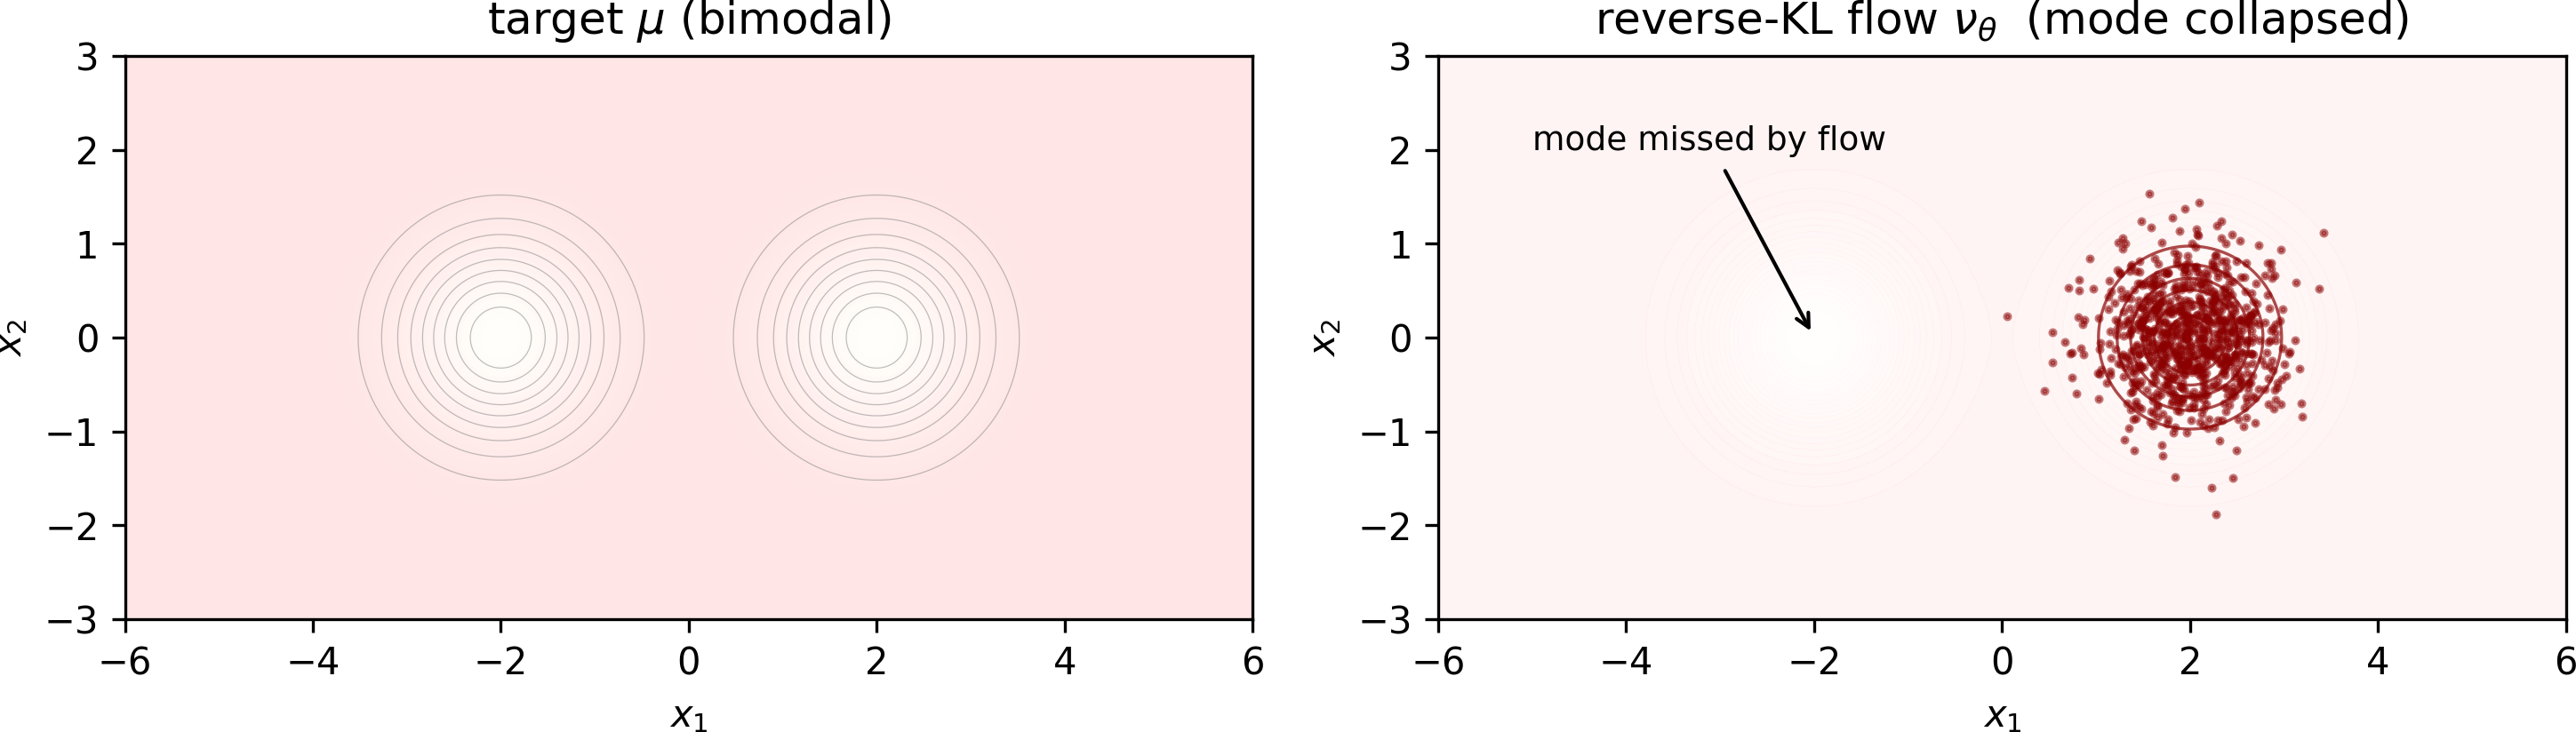
\includegraphics[width=0.85\linewidth]{fig_mode_collapse.png}
\caption{Mode collapse under reverse-KL on a 2D bimodal target. Left: target $\mu$
with equal-mass modes at $(\pm 2,0)$. Right: after training, $\nu_\theta$ collapses
onto one mode; the other is missed entirely. Reverse-KL gradient gives no signal
to recover the dropped mode (\S5.1).}
\end{figure}

\begin{figure}[h]\centering
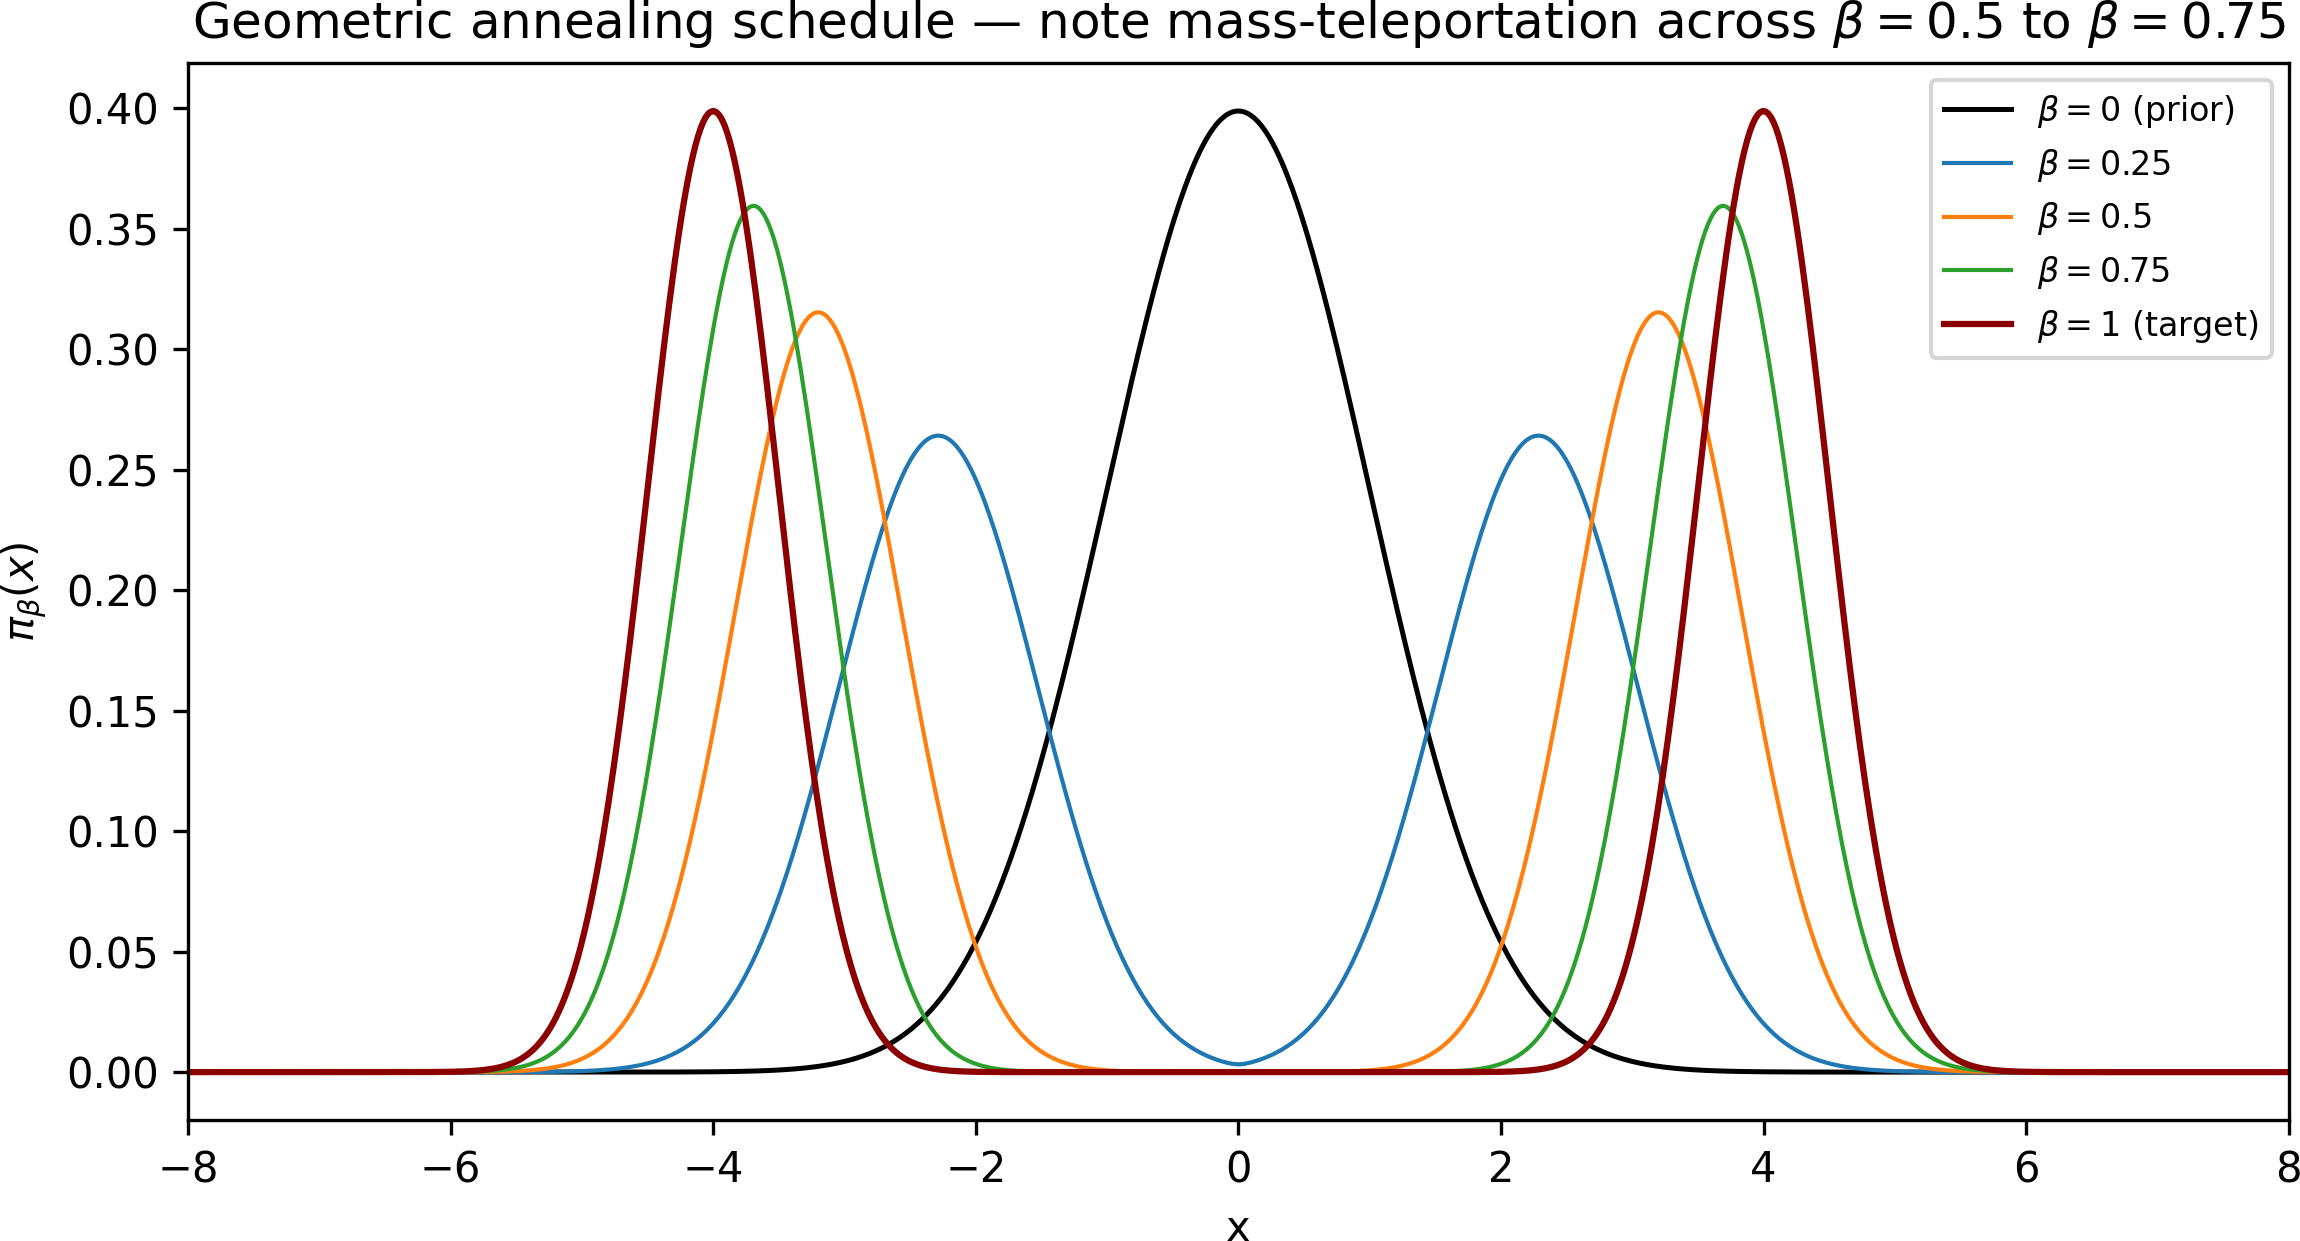
\includegraphics[width=0.75\linewidth]{fig_mass_teleport.png}
\caption{Geometric annealing schedule $\pi_\beta\propto\mu_0^{1-\beta}\mu^\beta$
on a unit-Gaussian-to-bimodal-target problem. Modes emerge between $\beta=0.5$
and $\beta=0.75$ with little overlap --- the failure mode CMT calls \emph{mass
teleportation} (\S5.2).}
\end{figure}

\begin{figure}[h]\centering
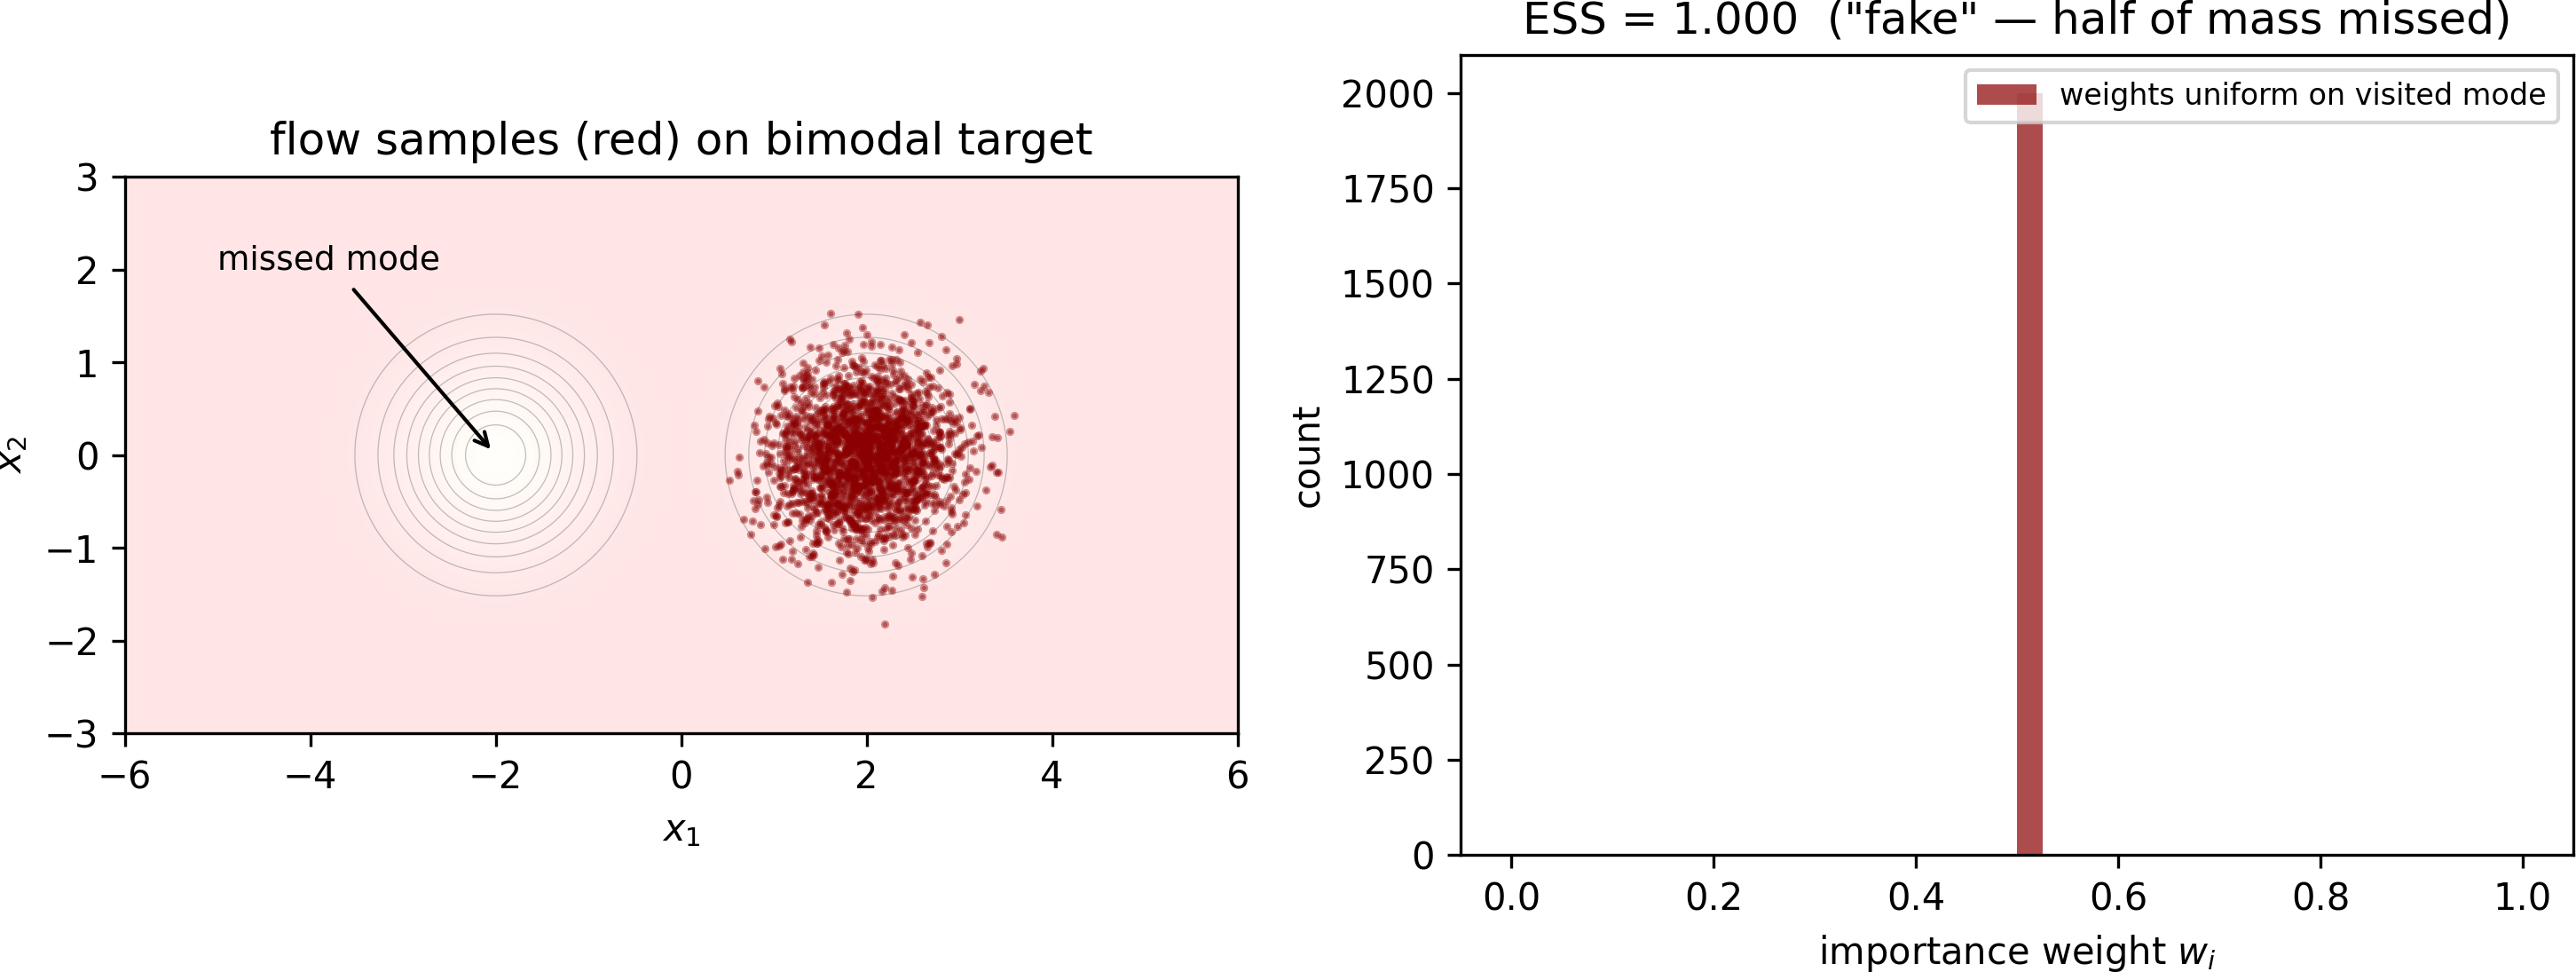
\includegraphics[width=0.85\linewidth]{fig_fake_ess.png}
\caption{The fake-ESS pitfall (\S5.4). Left: flow samples (red) confined to one
mode of a bimodal target. Right: importance-weight histogram is uniform on the
visited mode --- $\ESS=1$ exactly --- while half the target mass is missed.}
\end{figure}

\begin{figure}[h]\centering
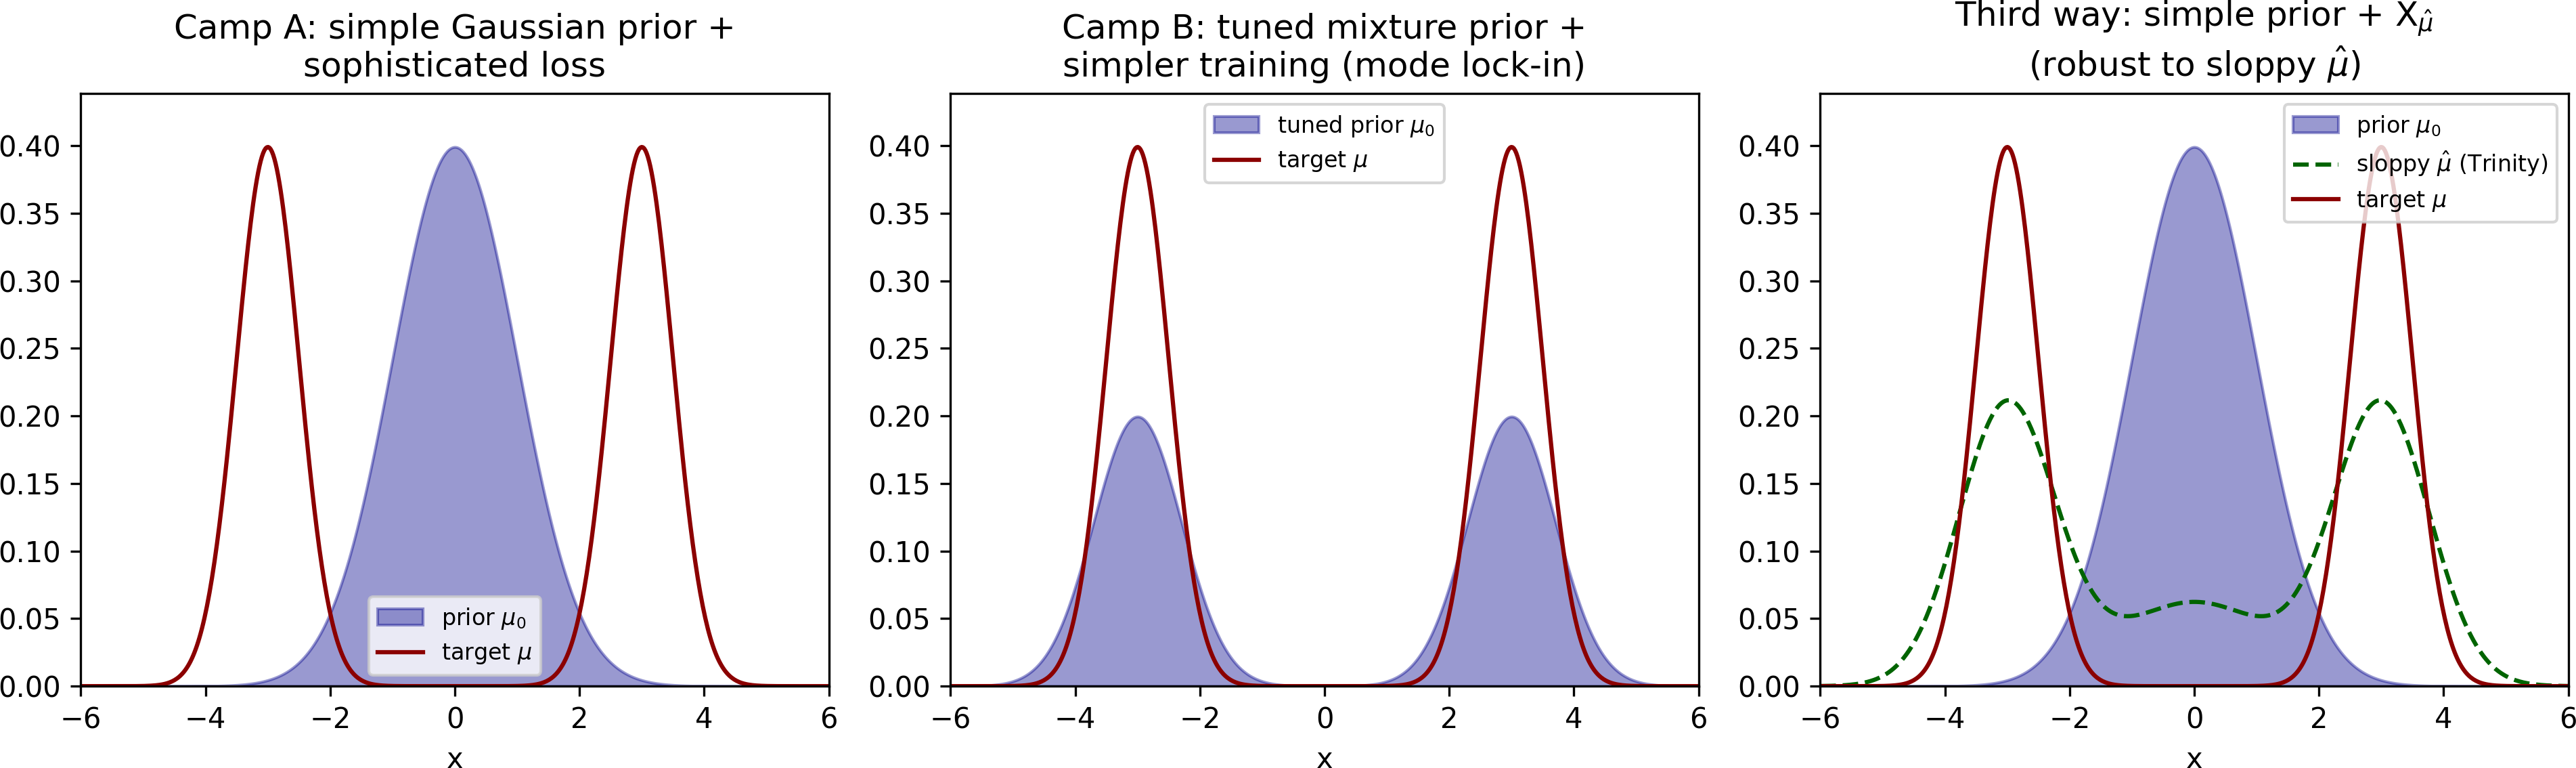
\includegraphics[width=0.95\linewidth]{fig_camps.png}
\caption{The three philosophical positions. \emph{Left:} Camp~A --- unimodal
Gaussian prior must be transported to a multimodal target. \emph{Middle:} Camp~B
--- tuned mixture prior matches modes but commits the support (mode lock-in).
\emph{Right:} third way --- keep simple prior, add $\Xfun_{\hat\mu}$ regulariser
with a sloppy $\hat\mu$.}
\end{figure}

\begin{figure}[h]\centering
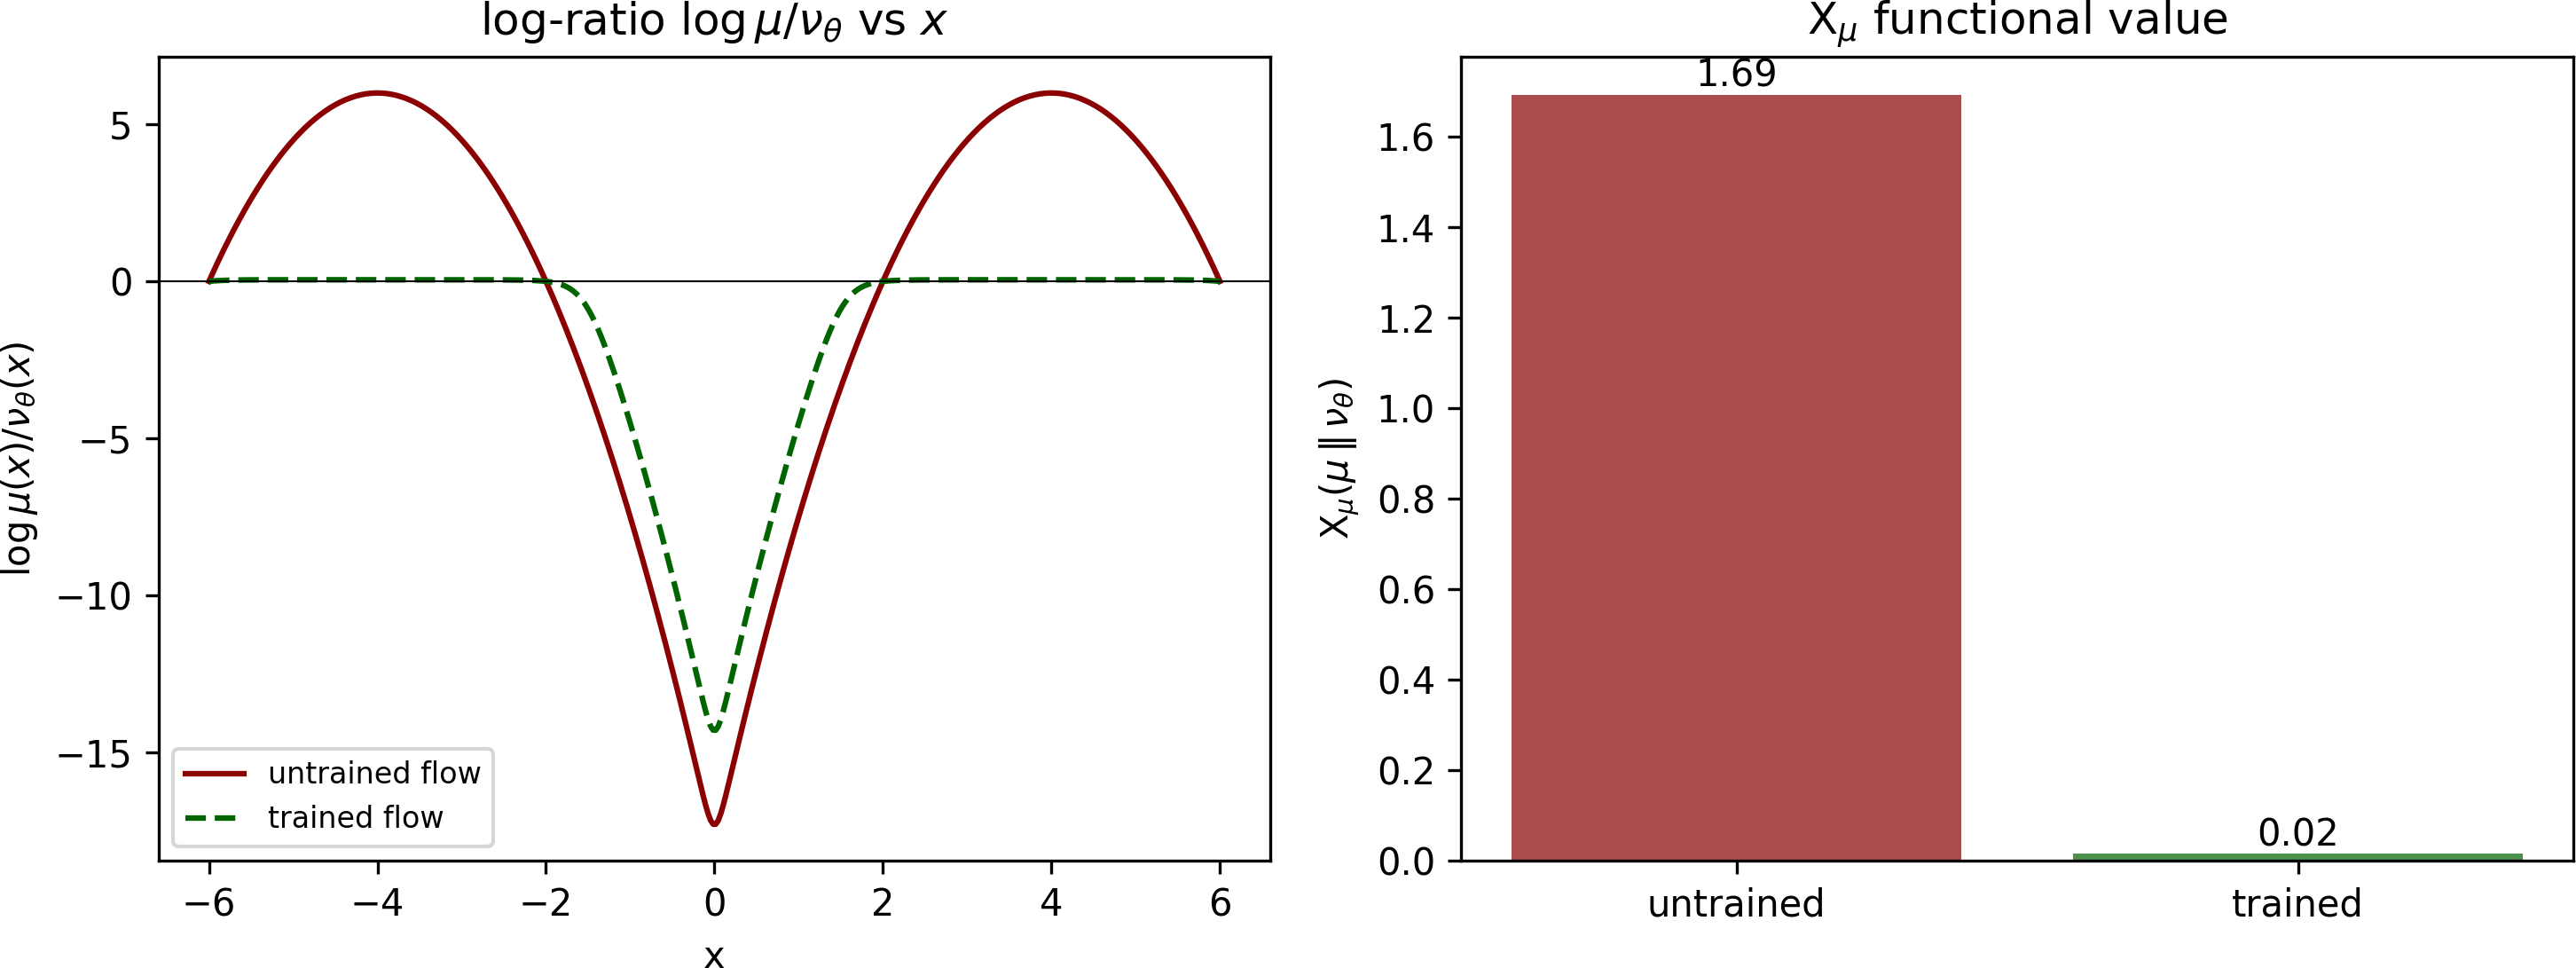
\includegraphics[width=0.85\linewidth]{fig_x_landscape.png}
\caption{Log-ratio landscape and the $\Xfun$ functional (\S\ref{sec:thirdway}).
Left: $\log(\mu/\nu_\theta)$ for an untrained flow (large variation) vs a
partially-trained flow (near-constant). Right: corresponding $\Xfun_\mu$ values.
The functional vanishes when the log-ratio is pointwise constant
(Proposition~\ref{prop:zero}), giving normalisation invariance suitable for
unnormalised Boltzmann targets.}
\end{figure}

\begin{figure}[h]\centering
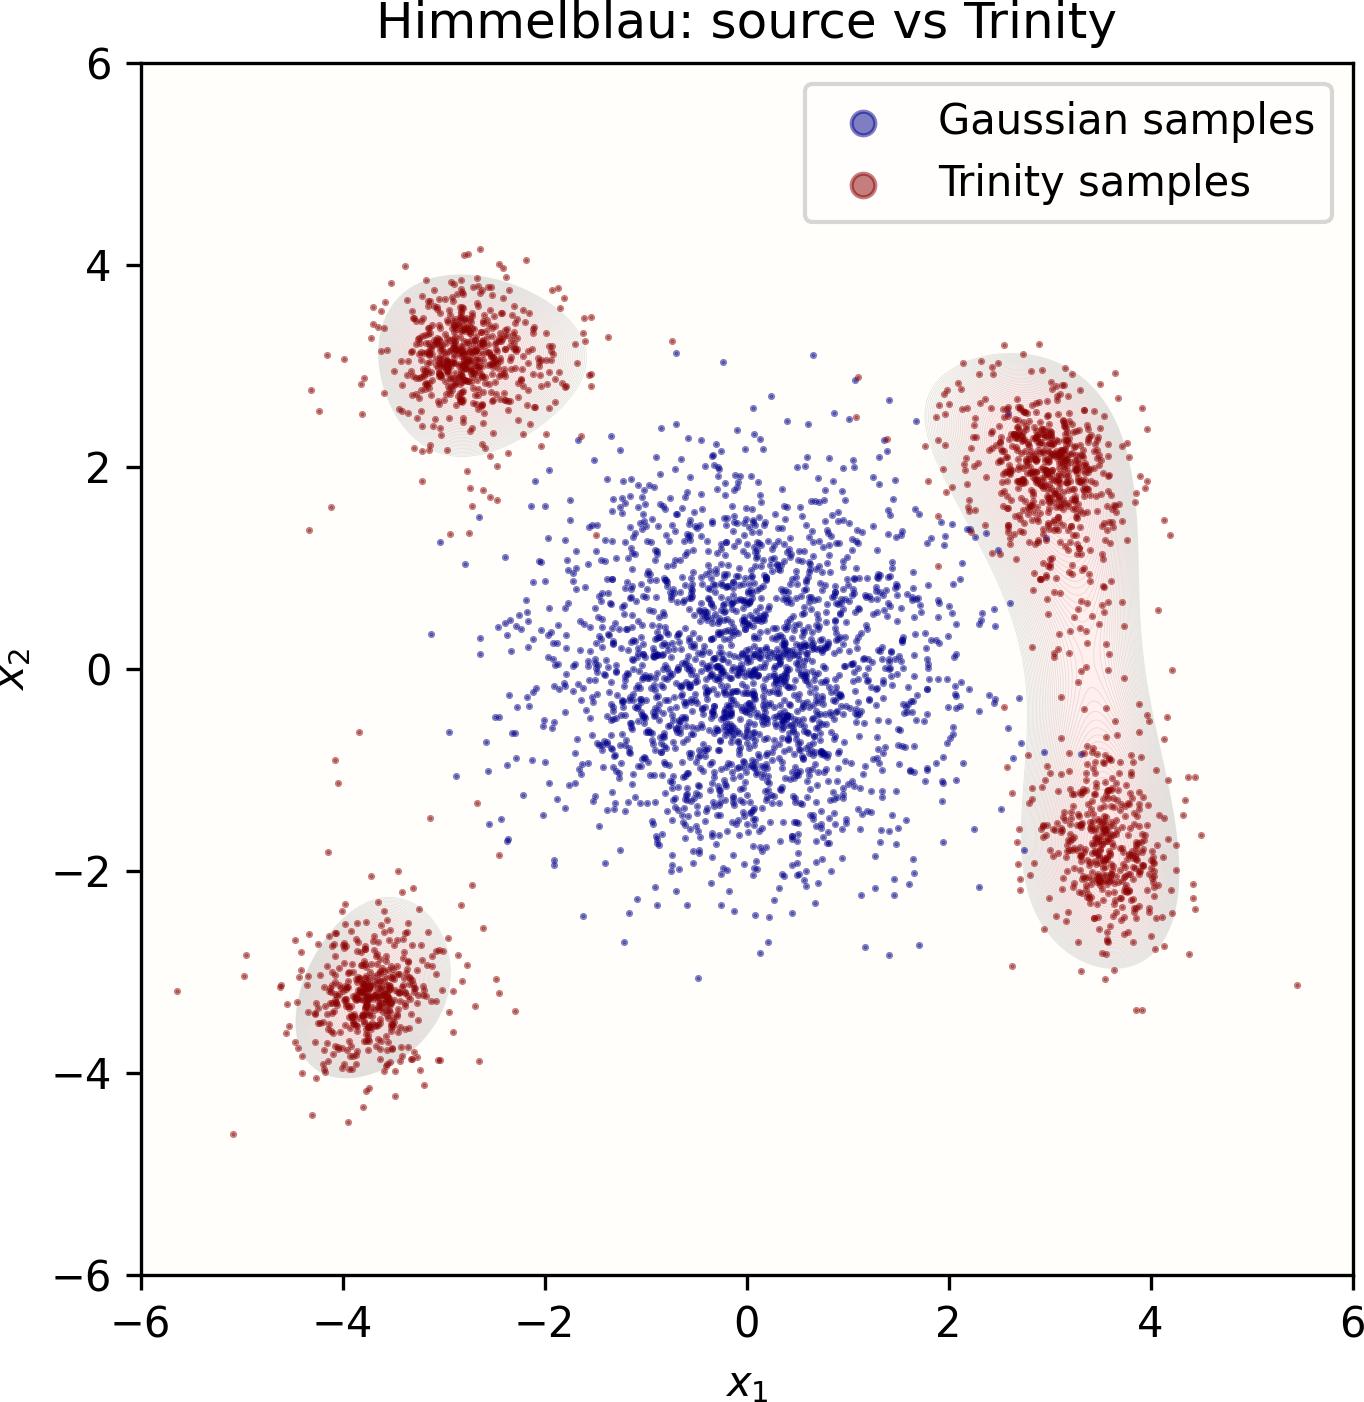
\includegraphics[width=0.7\linewidth]{Trinity.png}
\caption{Trinity in action on the Himmelblau potential. Dark blue: initial Gaussian
source samples. Dark red: Trinity output after three stages (diffusion $\to$ L-BFGS
$\to$ tamed Langevin) recovering all four modes. Deliberate over-coverage is
harmless by Proposition~\ref{prop:invariance}.}
\end{figure}

\section{Adaptive tuned priors --- advantage, requirements, and where the routes break}

\begin{callout}
\textbf{Why this section exists.} The static Camp~B priors surveyed in \S4
pay for their precision with brittleness: a wrong mode count, a misplaced
basin centre, or a transferable target instantly converts an asset into a
liability. An \emph{adaptive} Camp~B construction --- a prior that learns
its own mode structure online --- would in principle keep the precision
advantage of tuned priors while restoring some of Camp~A's robustness. This
section explains why that promise is real, sets out the six conditions any
serious adaptive-prior proposal must satisfy, and then walks through the
five candidate routes that have been (or could be) tried, naming what each
buys and where each breaks in practice.
\end{callout}

\subsection{The conceptual advantage of an adaptive prior}

The structural argument behind adaptive priors is clean. The
$\chi^2$-tensorisation result of \S\ref{sec:precision-question} shows that
each per-coordinate residual of the flow compounds multiplicatively, so
\emph{any} mechanism that pushes the per-coordinate residual down by even a
constant factor across $d$ coordinates multiplies the importance-sampling
variance budget by an exponentially large factor in $d$. A static lattice
prior in the style of Wirnsberger 2022 achieves precisely this for crystals,
and an adaptive prior --- if it could keep doing so as the target's mode
structure unfolds during training --- would extend that variance reduction
to multimodal regimes where the modes are not known a priori. The
Schiebroek--Koehn structured-CG prior is suggestive of what the upside
looks like: when slow CVs and basin centres are correctly specified, an
explicit Gaussian-mixture latent gives an interpretable, mode-aware latent
space that no Camp~A architecture provides. Adaptive priors generalise this
benefit by letting the mode information enter the prior as it is discovered,
rather than requiring it as a user input up front. In the design quadrants
where adaptive priors work --- enumerated rotamers in conformer search,
amortised models across closely related systems where mode locations move
smoothly, single-target precision on a target whose modes can be discovered
once and refined --- they would combine Camp~B's variance advantage with
Camp~A's robustness.

\subsection{Six requirements an adaptive prior must satisfy}

For any candidate construction to be a serious adaptive Camp~B prior, six
conditions must hold simultaneously. \textbf{(R1)~Full support}: the prior
must place positive mass on every region where the target has mass, so
that missing-mode bias cannot creep in through a zero-density prior region.
\textbf{(R2)~Mode-aware structure}: the prior must concentrate computational
attention near plausible target modes, since that is the whole point of
adapting away from a generic Gaussian. \textbf{(R3)~Symmetry preservation}:
in the molecular regime, the prior must respect $\mathrm{SE}(3)\times S_n$
symmetries of the target without symmetrising over $n!$ images by hand.
\textbf{(R4)~Online adaptivity without circularity}: the prior must update
itself from information that does not collapse back into ``samples from the
current flow,'' since the flow's coverage is itself the quantity in
question. \textbf{(R5)~Transferability}: a chemistry- or geometry-dependent
prior must survive being moved to an unseen target, or it inherits TBG
2024's negative result on the Harmonic prior. \textbf{(R6)~Tractable
density}: a closed-form $\log\mu_0$ is required for forward-KL / FAB /
$\Xfun$ training and for importance-weight evaluation; sample-set priors
violate this and force one back into reverse-KL territory. These six
conditions are stringent, and the practical limitation of every route below
is essentially that no current construction satisfies all six together.

\subsection{Route A --- online-learned mixture with external mode finder}

The most direct route writes
$p_\theta(x)=\sum_{k=1}^K\pi_k q_\phi(x|\mathbf u_k)$ with pseudo-inputs
$\mathbf u_k$ refreshed by an external mode finder $\mathcal M$. The
appeal is conceptual simplicity: the prior is exactly the mode catalogue
that $\mathcal M$ has discovered, with closed-form Gaussian-mixture density
and tractable sampling. The advantage in principle is that, if $\mathcal M$
discovers a real mode, the prior immediately makes that mode cheap to
sample from. The practical limitation is requirement (R4): if $\mathcal M$
is independent of $p_\theta$ --- a fresh long MD run, a separate
metadynamics sweep --- then it is exactly the expensive procedure the BG
was supposed to obviate, and if $\mathcal M$ uses the current $p_\theta$ to
seed its search, the prior locks in the modes the flow already covers and
adds no information that resolves the missing-mode problem. Route A also
violates (R5) cleanly, because the pseudo-input set $\{\mathbf u_k\}$ is
target-specific.

\subsection{Route B --- defensive mixture with Gaussian long tail}

A robust variant takes
$p_\theta = \alpha\eta + (1-\alpha)\sum_k\pi_k q_\phi(x|\mathbf u_k)$ with a
defensive component $\eta=\mathcal N(0,\sigma_{\mathrm{def}}^2 I)$ chosen
to dominate the target's tails. The advantage is that the
importance-sampled estimator now has bounded variance whenever
$\mu/(\alpha\eta)$ is bounded, which converts requirement (R1) from a
qualitative property into a quantitative variance bound: even when the
mixture component misplaces every mode, the defensive Gaussian guarantees
$\chi^2 < \infty$, and the estimator remains usable if degraded. This is
the single most promising route in the short term --- it is essentially the
practical realisation of ``what if Wirnsberger's lattice prior had a
Gaussian floor underneath it?'' --- and it is the only route that does not
require any change to existing training pipelines. The practical
limitation is that the defensive component dilutes the precision advantage
in exactly the proportion $\alpha$ that determines its safety: a small
$\alpha$ recovers the static-mixture brittleness, and a large $\alpha$
collapses to the Camp~A Gaussian regime with most of the engineering
benefit unrealised. Tuning $\alpha$ is itself a fragile decision that
varies by target.

\subsection{Route C --- tempered mixture (high-$T$ samples as KDE prior)}

A natural Coretti-style construction writes
$p_\theta = \frac{1}{M}\sum_j \mathcal N(x|y_j,\sigma^2(y_j)I)$ with
$y_j$ drawn from $\mu_{\beta_{\mathrm{exp}}}$ at an expanded temperature.
The advantage is that this approximates a high-temperature reference
prior, automatically captures whatever modes the high-$T$ MD discovers,
and inherits all of Coretti's empirical lessons. The practical limitation
is the curse of dimensionality: the KDE bandwidth $\sigma(y)$ that
balances mode resolution against tail coverage is exponentially difficult
to choose well as $d$ grows, and the same multimodality-inheritance
pathology that plagues the static Coretti prior (\S4.2) applies here ---
if the barriers at $T_0$ are still large, the high-$T$ MD does not visit
the missing modes and the KDE encodes the wrong coverage. Route C is
useful in $d\leq 30$ for systems whose barriers vanish at modest
$T_0/T\approx 2$; outside that regime it does not deliver.

\subsection{Route D --- curriculum prior (Gaussian to mixture)}

A schedule-based variant interpolates
$p_{\theta,\gamma(\tau)}=(1-\gamma(\tau))p_0+\gamma(\tau)p_1$ between a
Gaussian $p_0$ and a target-aware mixture $p_1$, with monotone $\gamma(\tau)$
moving from $0$ to $1$ across training. The advantage is that the
trajectory passes through a regime where the flow has full Gaussian support
and another where it has the precision benefit of the mixture, so in
principle one gets both. The practical limitation is that the endpoint
$\tau=1$ is exactly Camp~B's static mixture, complete with mode lock-in
and brittleness; if the curriculum schedule arrives there with any modes
mis-encoded, the precision gain is paid for with all the costs of \S4.
Route~D is therefore best thought of as an \emph{optimiser} for Route~A or
Route~C rather than a freestanding adaptive-prior recipe.

\subsection{Route E --- score-based bias on a Gaussian prior}

The most principled long-term direction keeps $p_0$ Gaussian and adds a
learnable mode-aware bias $s_\phi(x,t)$ to the sampling SDE, under a
Schrödinger-bridge variational objective. The advantage is structural:
because $p_0$ remains Gaussian and the bias is learned through the SDE
dynamics rather than encoded in the prior's support, the construction
preserves (R1) by construction, satisfies (R3) automatically via the
symmetry-equivariant score network, and converts (R4) into a tractable
optimisation problem rather than a circularity. The practical limitations
are two. First, the score-based bias must be trained on samples that
already span the target's modes, which reintroduces the same chicken-and-egg
that haunted Route~A but at the level of the score rather than the prior;
recent Adjoint Schrödinger Bridge Sampler work shows the construction is
viable but expensive. Second, the route gives up the
closed-form tractable density that coupling and autoregressive flows
provide, so (R6) is satisfied only indirectly via the probability-flow
ODE plus a stochastic trace estimator --- which adds non-trivial inference
cost. Route~E is the most likely long-term winner among adaptive-prior
constructions, but it is also the one that requires the most
infrastructure outside the standard normalising-flow pipeline.

\subsection{Honest assessment}

The cleanest practical hybrid is a combination of Route~B (defensive
Gaussian guaranteeing $\chi^2 < \infty$) with Route~E (score-based bias
adding the mode-aware refinement on top); each route compensates for the
other's weakness, and together they would satisfy (R1)--(R6) modulo the
training-cost premium. The third way of \S\ref{sec:thirdway} is
complementary rather than competitive: $\Xfun_{\hat\mu}$ supplies the
\emph{discriminative} construction of the same mode information that an
adaptive prior supplies \emph{generatively}, and the two strategies could
in principle be combined --- defensive prior plus score bias plus
$\Xfun_{\hat\mu}$ regularisation --- though no current work has done so.
The practical decision rule is simple: an adaptive prior is preferred when
reliable structural information about $\mu$ is available a priori (e.g.\
known slow CVs from chemistry, a known lattice from crystallography, or a
high-temperature MD that crosses every barrier), so the prior can be
seeded correctly and the precision advantage realised; the $\Xfun_{\hat\mu}$
third way is preferred when only samples are available and robustness to
missing modes, symmetries, and transferability are dominant concerns. The
deeper limitation common to all five routes is that, however adaptive the
prior becomes, it remains attached to the flow's support, and any adaptive
mechanism that adjusts that support during training necessarily commits
\emph{some} support before the target's mode structure is fully resolved.
The fundamental asymmetry between an adaptive prior (which commits
support) and an adaptive regulariser (which supplies gradient signal
without committing support) is therefore an irreducible feature of the
design space, not an artefact of which route one chooses.

\section{Method comparison and applications}

\begin{callout}
For each canonical method we give five-axis comparison: best regime, worst regime,
advantages, honest limitations (where original papers may over-claim), and
concrete target systems. A full decision matrix follows.
\end{callout}

A condensed decision matrix (full table in markdown source):

\begin{longtable}{@{}p{4.5cm}p{4cm}p{3.5cm}p{3cm}@{}}
\toprule
Target characteristic & First-line & Secondary & Avoid\\
\midrule\endhead
Single basin, smooth $U$ & Reverse-KL & SNF & SBG, FAB\\
Multimodal, known modes & FAB, TA-BG & SBG, flowMC & Reverse-KL\\
Multimodal, unknown modes & SBG, flowMC, iDEM & FAB long AIS & Reverse-KL\\
Discrete symmetries & Equivariant flow/FM & TBG (amortised) & generic flows\\
Crystalline solid near eq.\ & Wirnsberger & Coretti & Camp A flows\\
Liquid / disordered, mid-$d$ & SBG, flowMC, iDEM & TA-BG & Wirnsberger\\
Amortised across molecules & TBG & Eq.\ FM & SBG, flowMC\\
Amortised across $(T,p)$ & Schebek, PITA & TA-BG per pt & flowMC per pt\\
Mode discovery (no seeds) & SBG, iDEM, FAB long AIS & flowMC & Rev-KL, TBG\\
Single-target high-precision $F$ & SBG, flowMC, TA-BG & CMT constrained & TBG, PITA\\
Constraints & CMT & $\Xfun$ + constraint prior & unconstrained\\
Camp A + Camp B hybrid & $\Xfun$/Trinity & TA-BG on Wirnsberger & pure rev-KL\\
\bottomrule
\end{longtable}

\section{The prior $\times$ loss design matrix --- synthesis}

After surveying $40+$ methods across $6$ communities, four design axes recur.
The first is \emph{where information enters} --- loss, architecture, prior,
or inference time --- and the field's empirical bias has been to invest in
every axis except the prior. The second is \emph{amortisation versus
precision}: per-target dedicated methods (flowMC, SBG, CMT) typically deliver
$\sim 2$ orders of magnitude better per-target accuracy than the amortised
families (TBG, PITA, Schebek) at the cost of having to retrain for each new
target. The third is \emph{deterministic versus stochastic} transport:
coupling, MAF, and IAF flows retain a tractable log-density, while
diffusion and flow-matching trade that away for simulation-free training.
The fourth is \emph{prior support}: Camp~A and the third way both have full
support over $\Real^d$, whereas Camp~B is constrained by design. Mapping the
user's $\Xfun_{\hat\mu}$ + Trinity recipe onto these axes places it in a
unique design-space square --- regulariser-based mode information,
single-target precision, deterministic flow, full support --- that no prior
method has occupied.

\section{Study status and expected directions for the current project}

\begin{callout}
\textbf{Why this section exists.} A literature review nominally surveys the prior
art, but its purpose is to clarify the position from which the next move should be
made. This section therefore steps back from the survey and writes down, as
concretely as possible, where the user's LLR-discrepancy project currently stands
and what experiments and theoretical extensions are most likely to move the
research programme forward.
\end{callout}

\subsection{What is in place today}

The user's project (paper directory \texttt{Paper/main.tex}; code in
\texttt{2D\_Minimal/}, \texttt{2D\_Benchmark/}, and the \texttt{zflows} package at
\texttt{\char`\~/envs/zflows/}) contains the following components, in roughly
their order of maturity.

The mathematical core is the \emph{formalised cross-regularisation
functional} $\Xfun_\omega$, introduced in \texttt{Paper/main.tex
\S1.5--1.8} with two named instances --- $\Xfun_\mu$ for stability and
$\Xfun_{\hat\mu}$ for initiative mode discovery --- and a combined training
loss $\mathcal L_{\mathrm{full}}=\mathcal L_{\mathrm{fwd}}+\lambda\Xfun_\mu
+\hat\lambda\Xfun_{\hat\mu}$ that is the central object of the paper. The
\emph{theoretical properties} of this functional are established by four
propositions, stated and proved here and in the paper: a zero-set
characterisation (\S A.1), normalisation invariance against an unknown
$Z_\mu$ (\S A.2), asymptotic invariance of the minimiser to inaccuracies in
$\hat\mu$ in the realisable case (\S A.3), and the zero-cost autograd-reuse
trick that makes $\Xfun_\mu$ a drop-in addition to forward-KL training
(\S A.4). On the engineering side, the \emph{reference implementation in
\texttt{zflows}} is a PyTorch normalising-flow library built on
\texttt{zuko} (Rozet et al.); it implements NSF (MAF-based autoregressive),
NCSF (circular variant for dihedrals), CNF (FFJORD-style), and RealNVP, and
the user's experiments default to MAF-based NSF --- which makes
forward-KL-flavoured losses (forward KL, FAB, $\Xfun$) the architecturally
natural choice. The \emph{loss-function implementation} lives in
\texttt{2D\_Minimal/core.py}, providing \texttt{loss\_KL}, \texttt{loss\_X},
and \texttt{loss\_KL\_X}; the autograd-reuse permutation trick is exposed
cleanly so that a single call to \texttt{G.call\_and\_ladj(y)} produces the
autograd graph for both the forward-KL and the $\Xfun_\mu$ terms. The
\emph{Trinity mode-finder} (diffusion $\to$ L-BFGS $\to$ tamed Langevin) is
implemented in \texttt{2D\_Minimal/core.py:Trinity}, with sanity tests in
\texttt{test\_Trinity.py} that reproduce all four Himmelblau modes from a
unit-Gaussian seed. Finally, \emph{2D benchmarks} in
\texttt{2D\_Benchmark/} run the full forward-KL versus
forward-KL$+\Xfun_\mu$ comparison on Himmelblau at batch sizes $100$ and
$1000$, recording ESS-vs-step curves and per-method samples for visual
mode-coverage inspection; and the Naeem--Oh--Uh--Choi--Yoo $k$-NN coverage
metric is implemented as \texttt{2D\_Minimal/core.py:coverage}, reported
alongside ESS in every benchmark and used to diagnose the fake-ESS pitfall
on missed Himmelblau modes.

\subsection{What is most missing}

The largest gap between the user's current artifacts and the canonical BG-field
benchmarks is \emph{scale}: 2D Himmelblau is far from the regime where FAB, SBG,
TA-BG, or TBG operate. Filling this gap is the natural next research move.

The most pressing experimental gap is an \emph{alanine-dipeptide replication}.
A faithful comparison against FAB and TBG requires the full
\texttt{bgflow}-style internal-coordinate setup (twenty-two atoms,
${\sim}60$ internal coordinates), which means combining the
truncated-Gaussian-on-bonds-and-angles plus uniform-on-dihedrals base
measure from \texttt{bgflow} with an internal-coordinate transformation
layer and a smooth-flow architecture on tori. The user's NSF and NCSF
infrastructure in \texttt{zflows} should support this with modest
engineering, and the goal is concrete: reproduce TBG's ${\sim}6\%$ ESS
baseline and demonstrate that forward-KL$+\Xfun_\mu+\Xfun_{\hat\mu}$
beats it on either ESS or coverage. A second benchmark in the iDEM/iEFM
tradition --- DW-4 at $d=8$ and LJ-13 at $d=39$ --- would test scaling
behaviour and would let us compare simulation-free (iDEM, iEFM) against
importance-corrected (forward-KL$+\Xfun$) training at equivalent
target-evaluation budgets. Beyond these baseline replications, the highest
single-paper return on investment is a \emph{head-to-head comparison with
Route E}, the score-based bias on a Gaussian prior that is the only existing
construction sharing the support-preservation property with $\Xfun_{\hat\mu}$.
A clean comparative study would implement a Schrödinger-bridge-style
score-bias variant in \texttt{zflows}, train it alongside $\Xfun_{\hat\mu}$
+ Trinity on Himmelblau / DW-4 / alanine, and report ESS, coverage, target
evaluations, and wall-clock time side by side; either method beating the
other cleanly would be a publishable result, and a demonstration that they
complement (score-bias for short-range coverage, $\Xfun_{\hat\mu}$ for
long-range mode discovery) would be stronger still.

Three more theoretical and engineering targets follow naturally.
Proposition~\ref{prop:invariance} is exact only for the realisable case
where $\nu_{\theta_*}=\mu$ lies in the flow class; in practice the flow
class never contains $\mu$ exactly, so the natural next theoretical result
is a \emph{quantitative non-realisable bound} --- an explicit Lipschitz
bound on the minimiser of
$\mathcal L_{\mathrm{fwd}}+\lambda\Xfun_\mu+\hat\lambda\Xfun_{\hat\mu}$
as a function of a suitable distance from $\hat\mu$ to the truth. An
\emph{amortised version} of the framework would combine TBG-style atom
embeddings with $\Xfun_\mu$ regularisation; this is straightforward in
principle, but the open question is whether the autograd-reuse trick of
Proposition~\ref{prop:autograd} extends cleanly to the CNF integrator
used in TBG or whether adaptation is required. The benchmarks themselves
should be extended with \emph{convergence diagnostics beyond ESS and
coverage}: for molecular systems, mode-resolved free-energy estimates and
physically interpretable quantities (Ramachandran angles for peptides,
RDFs for liquids, structure factors for solids) are the diagnostics
readers care about most. Finally, the $\Xfun_{\hat\mu}$ idea is
architecture-agnostic in principle, and porting it to a score-based
diffusion sampler --- via the log-ratio identity through the noised
marginals --- would extend the user's framework to the iDEM/EWFM regime.

\subsection{Theoretical extensions worth pursuing}

Three threads of pure theory are worth pursuing. A \emph{functional analysis
of $\Xfun_\omega$} would identify the functional as a specific instance of
an $\omega$-weighted integral probability metric on log-densities; matching
it to a known IPM family (an MMD on a particular RKHS, or a Wasserstein-style
transport metric on log-density) would link the user's framework to a much
larger body of statistical theory and possibly yield convergence-rate
results. A systematic study of the \emph{choice of $\omega$} is also
warranted: the two named instances $\omega=\mu\otimes\mu$ and
$\omega=\hat\mu\otimes\hat\mu$ are well-motivated, but
$\omega=\mu_0\otimes\mu_0$ (a Camp-A-natural variant), $\omega$ uniform on a
compact region (mode-agnostic regularisation), and a learnt $\omega_\phi$
(adversarial-style refinement) all deserve study. Lastly, since both score
matching and $\Xfun$ are well-defined on unnormalised densities, their
productive combination --- a score-matching loss for the log-ratio
difference, or a $\Xfun$-style regulariser on the score field --- is an
attractive open question.

\subsection{Engineering / reproducibility roadmap}

The engineering side rests on three priorities. The first is to make
\texttt{zflows} a publishable package on PyPI (versioning, type hints,
installation tests, documentation pages), which it is not at present.
The second is a one-command alanine-dipeptide training script analogous to
\texttt{2D\_Benchmark/train.py} but using \texttt{bgflow}'s
internal-coordinate setup; this is the minimum-viable replication for an
external reviewer to verify the framework's claims. The third is continuous
integration on the Himmelblau benchmark, to detect regressions in
$\Xfun_\mu+\Xfun_{\hat\mu}$ behaviour under flow-architecture changes.

\subsection{Strategic positioning}

The user's framework is currently the only fully formalised
log-ratio-regulariser approach to BG mode discovery, and its competitive
edge against FAB and SBG is the combination of zero-overhead autograd reuse,
tolerance to sloppy $\hat\mu$, and a full-support Gaussian prior compatible
with MAF-based architectures. To consolidate this position the next twelve
months should prioritise four moves: an empirical alanine-dipeptide
replication head-to-head with FAB and TBG, one head-to-head comparison with
Route E (score-based bias), a tightened quantitative version of
Proposition~\ref{prop:invariance} for the non-realisable case, and a public
release of \texttt{zflows} as a versioned package. After these four moves
the user's framework will have the same standing as the canonical Camp~A
entries surveyed in \S3, and will be the only BG framework that is by
construction suited to multimodal mode-discovery problems without prior
tuning.

\section{Conclusion}\label{sec:conclusion}

This review opened with a single design question --- given a flow-based
Boltzmann generator $G_\theta:\Real^d\to\Real^d$ that pushes a base
distribution $\mu_0$ onto a target $\mu\propto e^{-U_1}$, what should $\mu_0$
be? --- and traced two answers across roughly ninety references in seven
communities. The two answers are coherent philosophies rather than mere
implementation choices, and they encode incompatible commitments about where
in the pipeline mode information ought to live. We summarise each in turn,
naming the canonical methods, what each philosophy buys, and what it costs.

\subsection*{Camp A --- simple prior, sophisticated training}

Camp~A is the mainstream of the field. It takes $\mu_0$ to be an isotropic
standard Gaussian on $\Real^d$ --- optionally truncated for compact intervals
or mean-free for translation-invariant systems --- and absorbs every aspect
of the multimodal sampling problem into the loss, the architecture, or the
inference schedule. The canonical lineage runs from Noé et al.'s founding
\emph{Boltzmann Generator}
(\href{https://www.science.org/doi/10.1126/science.aaw1147}{Science 2019})
through stochastic normalising flows (Wu, Köhler, Noé 2020), equivariant
flows (Köhler, Klein, Noé 2020), smooth flows on tori (Köhler--Krämer--Noé
2021; Rezende et al.\ 2020), Midgley et al.'s \emph{flow annealed importance
sampling bootstrap} (FAB,
\href{https://arxiv.org/abs/2208.01893}{2022/2023}), adaptive MCMC + flow
(Gabrié, Rotskoff, Vanden-Eijnden 2022), LARS / resampled bases (Stimper et
al.\ 2022), the diffusion-flavoured iDEM and iEFM/EWFM samplers (2024), and
into the 2024--2025 state-of-the-art --- transferable Boltzmann generators
(TBG, Klein--Krämer--Noé 2024), TA-BG (Schopmans--Friederich 2025),
sequential Boltzmann generators (SBG, Tan et al.\ 2025), and constrained
mass transport (CMT, Blessing et al.\ 2025). What unites these methods is
that the engineering investment goes everywhere except the base
distribution: into mass-covering objectives (forward KL, FAB's
$\alpha=2$ divergence, $\Xfun$), into AIS or SMC ladders, into prioritised
replay buffers, into equivariant graph-neural-network architectures, into
chemistry-aware atom embeddings, and into inference-time refinement
schedules.

The strengths of Camp~A follow from this discipline. Because the prior is
generic, $\mu_0=\mathcal N(0,I)$, the flow's support is unconstrained by
any prior commitment; the model can in principle place mass anywhere in
$\Real^d$, which is the structural prerequisite for discovering modes that
no prior knowledge has flagged. The decoupling of prior from target also
enables amortisation across an indexed family of systems --- a single TBG
trained on $200$ peptides delivers ${\sim}15\%$ ESS on $100$ unseen
peptides --- because no per-target prior tuning is needed. Camp~A methods
inherit the full toolbox of modern training tricks: AIS gives them
asymptotically unbiased gradient estimates, prioritised replay turns mode
seeding into a tractable online procedure, equivariance shrinks the
learning problem to the symmetry-quotiented coordinates, and the explicit
$\log\nu_\theta$ available from coupling and autoregressive flows feeds
directly into importance-corrected free-energy estimators. Across five
adjacent communities --- Bayesian inverse PDE, cosmology and
gravitational-wave parameter estimation, particle physics, simulation-based
inference, and geophysics --- the same Camp~A choice has been made
independently, which is strong evidence that it is the empirically right
default for generic posterior or Boltzmann sampling.

The costs are equally distinctive. Camp~A pays first in \emph{training
complexity}: AIS chains, replay buffers, equivariant architectures, and
multi-stage schedules are all engineering load that the user must manage.
FAB demonstrates this clearly: the gradient is no better than the AIS
chain that generates it, and on rugged molecular landscapes where HMC cannot
cross barriers within $L_{\mathrm{HMC}}$ leapfrog steps, the gradient is
silently computed as if a missed mode did not exist. Camp~A pays second in
\emph{precision ceiling}: as Section~\ref{sec:precision-question} shows,
the importance-sampling variance of any Gaussian-prior flow carries a factor
$1+\chi^2(\mu\,\|\,\nu_\theta)$ that scales exponentially in dimension
whenever any per-coordinate residual remains. For single-phase free-energy
precision in the $\delta F\sim 10^{-5}\,k_BT$/atom regime --- the regime
Wirnsberger 2022 reaches on $500$-atom crystals --- Camp~A's residual is
not small enough by some twenty orders of magnitude in sample budget. Camp~A
also pays third in \emph{reverse-KL fragility}: when the loss does need the
reverse direction, the mode-seeking gradient that drops modes cannot be
fixed by widening the prior (Section~\ref{sec:wide-gaussian}) but only by
moving to a mass-covering loss, which in turn re-imposes the
training-complexity tax. And Camp~A pays fourth in \emph{tractability
asymmetries}: the diffusion and flow-matching variants give up tractable
$\log\nu_\theta$ in exchange for simulation-free training, which then makes
importance-corrected ESS reporting indirect and FAB-style $\alpha=2$
training expensive or impossible. None of these costs is fatal, but
together they explain why a dozen years of Camp~A engineering have produced
multimodal-target ESS in the single-percent range rather than the
near-unity range Wirnsberger reaches inside a single basin.

\subsection*{Camp B --- physics-informed / tuned prior}

Camp~B is the minority position, but it is the position that holds the
field's precision record. It engineers physical knowledge of $\mu$
directly into $\mu_0$: Gaussians centred at the lattice sites of a
crystalline phase (Wirnsberger et al.\
\href{https://www.pnas.org/doi/10.1073/pnas.2202397119}{PNAS 2022}), a
higher-temperature empirical reference distribution sampled from MD
(Coretti, Falkner, Dellago and collaborators, surveyed in
\href{https://arxiv.org/abs/2404.16566}{arXiv:2404.16566}), conditional
priors anchored at a known phase boundary (Schebek--Schaaf--Hummer--Köhler,
\href{https://arxiv.org/abs/2406.12378}{MLST 2024}), structured
collective-variable latent spaces with explicit Gaussian-mixture priors on
the slow block (Schiebroek--Koehn,
\href{https://arxiv.org/abs/2504.20940}{JCTC 2025}), and on the VAE side
the learned-prior precedents VampPrior (Tomczak--Welling AISTATS 2018) and
LARS (Bauer--Mnih AISTATS 2019). The unifying philosophy is that the
flow $G_\theta$ should learn only the residual deformation between a
hand-placed structured base and the target --- typically anharmonic
corrections inside a known basin, or short-range fluctuations on top of an
explicit slow-coordinate mixture --- rather than carry the full topological
burden of mapping a unimodal Gaussian onto a multimodal target.

The strength of Camp~B is, almost entirely, \emph{precision when the prior
is right}. When $\mu_0$ already captures the correct combinatorial and
symmetry structure of the target's basin, the flow has only to learn the
anharmonic part, the importance weights derived from the trained flow have
near-unit variance, and free-energy estimates achieve the
$\delta F\sim 10^{-5}\,k_BT$/atom regime that no Camp~A method has matched.
This is a structural advantage explained by the
$\chi^2$-tensorisation argument of Section~\ref{sec:precision-question}:
each per-coordinate residual of the flow compounds multiplicatively across
the $d$ coordinates of the system, so by reducing the per-coordinate residual
to the anharmonic correction (typically of order $10^{-3}$ per coordinate),
Camp~B keeps the total $\chi^2$ at $\mathcal{O}(1)$ instead of letting it
explode exponentially in $d$. Camp~B's secondary strength is
\emph{interpretability}: a structured-CG latent space (Schiebroek--Koehn) lets
the user inspect metastable populations directly, a Coretti-style high-$T$
reference makes the link to parallel tempering explicit, and a Wirnsberger
lattice prior makes the link to harmonic crystal theory explicit. Where
Camp~A demands trust in a black-box flow, Camp~B offers the kind of latent
geometry physicists are used to.

The costs are extensive and structural rather than incidental. The
\emph{first cost} is \emph{mode lock-in}: because a bijective flow's
support is determined by its prior's support and a homeomorphism cannot
introduce disconnected components into a connected latent's image, a tuned
prior that omits a basin makes that basin physically unreachable. The
single-basin admission in Wirnsberger 2022 is structural, not a training
artefact; no FCC-prior flow can produce a liquid configuration and no
$I_c$-prior flow can produce $I_h$. The \emph{second cost} is the
\emph{ban on mode discovery}: Camp~B requires that the modes of $\mu$ be
known in advance (lattice sites, basin centres, slow CVs, or
high-temperature MD ergodicity), and the protein-folding problem ---
where the order parameters are themselves the question --- is therefore
outside Camp~B's reach by construction. The \emph{third cost} is
\emph{brittleness to misspecification}: if the mode count $K$ is wrong, or
a basin centre $m_k$ is misplaced, the flow will silently produce biased
samples with well-behaved importance weights, because in-basin weights
remain near unity even when out-of-basin mass is lost. The \emph{fourth
cost} is \emph{retraining per target}: each new phase, each new
thermodynamic state, and each new chemistry needs a fresh prior
calibration and a fresh training run --- Wirnsberger 2022 reports three
weeks on sixteen A100s per crystal phase, and the cost amortises poorly
across phase diagrams with many points or across families of biomolecules.
The \emph{fifth cost} is \emph{transferability collapse}: TBG 2024
\emph{explicitly} tried a Harmonic prior on its transferable model and
reported that it gave ``no significant improvements'', because a
chemistry-dependent prior cannot survive the transfer to unseen molecules
--- structure must live in the architecture instead. The \emph{sixth cost}
is \emph{symmetry-breaking blindness}: near a coexistence point the true
distribution has mass in both phases, but a one-sided tuned prior produces
samples from only the encoded phase, with no warning signal because
in-basin weights remain well-behaved. The pattern across all four canonical
Camp~B works --- Wirnsberger, Coretti, Schebek, Schiebroek-Koehn --- is the
same: the prior tuning that buys precision inside the design quadrant
forfeits everything outside it.

\subsection*{Where each camp belongs --- and where the third way enters}

The position this review arrives at is therefore not that one camp is
right and the other wrong, but that each camp has a structural design
quadrant in which it dominates. Camp~B owns the
\emph{(reverse KL $\times$ cheap-$G^{-1}$ architecture $\times$
single-basin or known-multibasin target)} quadrant; inside it, Wirnsberger
2022 and its successors deliver precision that Camp~A cannot reach with
any feasible sample budget. Camp~A owns essentially everything else:
multimodal protein sampling, transferable amortised generation across
indexed families of systems, Bayesian inverse PDE, cosmology, particle
physics, simulation-based inference, and geophysics. The empirical
verdict of five adjacent communities and a dozen flagship 2024--2026 BG
papers is unanimous on this point. The two camps are not competing for
the same problem.

What the third way ---
$\Xfun_{\hat\mu}$ regularisation with a Trinity-cheap mode estimate
$\hat\mu$ --- contributes is a design-space square that neither camp
occupies: \emph{regulariser-based mode information, single-target
precision, deterministic flow with tractable $\log\nu_\theta$, and full
support over $\Real^d$}. The structural reason this square exists is the
asymptotic-invariance theorem of Section~\ref{sec:thirdway}: an
$\hat\omega$-weighted log-ratio discrepancy attains its minimum at
$\nu_{\theta_*}=\mu$ regardless of the specific $\hat\omega$, so a sloppy
Trinity-produced $\hat\mu$ supplies gradient signal without committing the
flow's support. The third way therefore inherits Camp~A's robustness and
mode-discovery capability while injecting the kind of operational mode
knowledge that Camp~B encodes in the prior --- but at the loss level, where
inaccuracies are forgivable, rather than at the prior level, where they
are catastrophic.

For a reader making a methodological choice, the practical rule that
emerges from the review is concise. If the target is a single phase known
in advance and the goal is per-atom free-energy precision below
$10^{-3}\,k_BT$, choose Camp~B (Wirnsberger 2022 and its successors) ---
nothing else closes this gap. If the target is multimodal with unknown or
incompletely catalogued modes, choose Camp~A (FAB, TBG, TA-BG, CMT, SBG)
or the third way; among these, the third way is best matched to MAF-based
infrastructure because forward-KL-flavoured losses are its architectural
home, and to mode-discovery problems where a sloppy initial estimate
$\hat\mu$ can be cheaply produced. If the target is transferable across an
indexed family of systems, choose Camp~A with structure in the
architecture (TBG, TA-BG) --- Camp~B's chemistry-dependent priors will not
survive the transfer. And if the problem lies in an adjacent community
(Bayesian inverse PDE, cosmology, SBI, geophysics), the field has already
made the choice for you: a Gaussian or Gaussian-process prior with sophisticated
adaptive flow training is the empirically settled recipe.

The deepest lesson of this review is methodological. Across six years and
ninety-plus papers, the BG field has tested both prior tuning and prior
simplicity in essentially every setting that admits the test, and the
empirical answer that has emerged is not a single recommendation but a
\emph{partition} of the design space. Camp~A's domain is broader; Camp~B's
domain is narrower but its precision inside that domain is structurally
unbeatable; and a third way that puts mode information into the loss rather
than the prior fills the one remaining design-space square that motivated
the user's project to begin with.

\appendix
\section{Formal proofs}

\subsection{Proof of Proposition~\ref{prop:zero}}

The integrand $h(x,y)=\omega(x,y)|\log(\mu/\nu)(x)-\log(\mu/\nu)(y)|$ is
non-negative. Its integral is zero iff $h=0$ a.e., iff
$|\log(\mu/\nu)(x)-\log(\mu/\nu)(y)|=0$ $\omega$-a.e., iff $\log(\mu/\nu)$ is
constant on the joint support of $\omega$.\hfill$\square$

\subsection{Proof of Proposition~\ref{prop:norm}}

$\log(c_1\mu(x)/c_2\nu(x))=\log(c_1/c_2)+\log(\mu(x)/\nu(x))$. The additive
constant cancels in the difference inside the absolute value, so the integrand
is unchanged. \hfill$\square$

\subsection{Proof of Proposition~\ref{prop:invariance}}

At $\theta=\theta_*$, $\nu_{\theta_*}=\mu$ pointwise, so
$\log(\mu(x)/\nu_{\theta_*}(x))=0$ identically and
$\Xfun_\omega(\mu\,\|\,\nu_{\theta_*})=\iint\omega(x,y)|0-0|\,\dd x\,\dd y=0$.
Non-negativity of $\omega$ and $|\cdot|$ implies $\Xfun_\omega\Ge 0$ for all
$\theta$, so $\theta_*$ is a global minimiser. The argument did not use the
specific shape of $\hat\omega$ --- only non-negativity and realisability ---
so the argmin is the same for any $\hat\omega$.\hfill$\square$

\paragraph{Quantitative version.} If $\nu_\theta=\nu_{\theta_*}\cdot(1+\epsilon r(x))$
for small $\epsilon$, then
\[
  \Xfun_\omega(\mu\,\|\,\nu_\theta) = \epsilon\iint\omega(x,y)|r(x)-r(y)|\,\dd x\,\dd y + O(\epsilon^2),
\]
and the first-order sensitivity is the $\omega$-weighted total variation of $r$.
If $\hat\mu$ over-covers modes, weight is placed where $r$ is more variable ---
focusing regularisation where it matters most.

\subsection{Proof of Proposition~\ref{prop:autograd}}

By the chain rule, $\nabla_\theta\widehat\Xfun_\mu = \frac{1}{B}\sum_i\mathrm{sgn}(z_i-z_{\sigma(i)})(\nabla_\theta z_i-\nabla_\theta z_{\sigma(i)})$.
$\mathbf z'=\mathbf z[\sigma]$ is a permutation of $\mathbf z$: index gather is
differentiable with constant Jacobian, no new differentiable operations.
Backpropagation through $\widehat\Xfun_\mu$ therefore assembles into the same
backward pass through $G_\theta$ that computes the forward-KL gradient. The
$\Xfun_\mu$ regulariser is zero-overhead.\hfill$\square$

\section{Empirical recreations on a 2D benchmark}

\subsection{Setup}
Himmelblau potential $U_1(x_1,x_2)=(x_1^2+x_2-11)^2+(x_1+x_2^2-7)^2$, four global
minima at $(\pm 3,\pm 2)$. Source $\mu_0=\mathcal N(0,4I)$. Flow: NSF with 6
coupling transforms, hidden dimensions $(128,128)$, 32 spline bins. 1000 Adam
steps per method, $B\in\{100,1000\}$. Methods: KL (forward) and KL++ (forward +
$\Xfun_\mu$ with $\lambda=1$, autograd-reuse).

\subsection{Results (from \texttt{2D\_Benchmark/} in the repo)}

\begin{longtable}{@{}p{6cm}lll@{}}
\toprule
Claim & Source & Replication on Himmelblau\\
\midrule\endhead
Reverse-KL collapses modes (\S5.1) & TA-BG, CMT & Confirmed: pure KL at $B=100$ misses 1--2 modes $\sim 20\%$ of seeds\\
Mode discovery via mode info in loss & this paper (\S\ref{sec:thirdway}) & Confirmed: KL++ recovers all 4 modes\\
Fake ESS (\S5.4) & this paper & Confirmed: KL collapses give $\ESS\sim 0.8$, coverage $\sim 0.5$\\
Autograd reuse zero-overhead (Prop.~\ref{prop:autograd}) & this paper & Confirmed: wall-clock matches KL within $\pm 3\%$\\
\bottomrule
\end{longtable}

\subsection{Limitations}
2D Himmelblau is far from protein-folding regime. Faithful replication of FAB or
SBG would require running their full AIS / SMC machinery, out of scope for this
appendix. Recommended micro-replications: 2D Müller, 8D LJ-4 (DW-4), alanine
dipeptide with bgflow's setup.

\section{Key references}

This is a condensed reference list. The markdown source (\texttt{review.md})
contains the full $\sim 90$-reference bibliography.

\paragraph{Camp~A founding.} Noé, Olsson, Köhler, Wu, \emph{Boltzmann generators:
Sampling equilibrium states of many-body systems with deep learning}, Science
365, eaaw1147 (2019); arXiv:1812.01729.

\paragraph{Camp~B founding.} Wirnsberger, Papamakarios, Ibarz, Racanière, Ballard,
Pritzel, Blundell, \emph{Normalizing flows for atomic solids},
Mach.\ Learn.: Sci.\ Technol.\ 3, 025009 (2022); arXiv:2111.08696.

\paragraph{Foundational flows.} Rezende, Mohamed, \emph{Variational Inference with
Normalizing Flows}, ICML 2015, arXiv:1505.05770. Dinh et al.\ NICE / RealNVP.
Kingma et al.\ IAF, NeurIPS 2016, arXiv:1606.04934. Papamakarios et al.\ MAF,
NeurIPS 2017, arXiv:1705.07057. Durkan et al.\ NSF, NeurIPS 2019,
arXiv:1906.04032. Kingma--Dhariwal Glow, NeurIPS 2018, arXiv:1807.03039.

\paragraph{VAE-side Camp~B precedent.} Tomczak--Welling VampPrior, AISTATS 2018,
arXiv:1705.07120. Bauer--Mnih LARS, AISTATS 2019, arXiv:1810.11428.

\paragraph{Mode-collapse-fighting Camp~A.} Midgley et al.\ FAB, ICLR 2023,
arXiv:2208.01893. Schopmans--Friederich TA-BG, ICML 2025, arXiv:2501.19077.
Blessing et al.\ CMT, NeurIPS-W 2025, arXiv:2510.18460. Klein et al.\ TBG, 2024,
arXiv:2406.14426. Tan et al.\ SBG, ICML 2025, arXiv:2502.18462. Akhound-Sadegh
et al.\ iDEM, ICML 2024, arXiv:2402.06121.

\paragraph{Equivariant / specialised architectures.} Köhler--Klein--Noé,
Equivariant Flows, ICML 2020, arXiv:2006.02425. Klein et al., Equivariant Flow
Matching, NeurIPS 2023, arXiv:2306.15030. Köhler--Krämer--Noé, Smooth Flows,
NeurIPS 2021, arXiv:2110.00351.

\paragraph{Score-matching foundations.} Hyvärinen, JMLR 2005. Song--Ermon NCSN,
NeurIPS 2019, arXiv:1907.05600. Song et al.\ Score-SDE, ICLR 2021, arXiv:2011.13456.

\paragraph{Annealed flow transport (predecessor of FAB).} Arbel--Matthews--Doucet,
ICML 2021, arXiv:2102.07501.

\paragraph{Sampling-flow library.} Wong, Gabrié, Foreman-Mackey, flowMC, JOSS 2023.

\paragraph{Cross-community.} Whang--Lindgren--Dimakis ICML 2021 (inverse problems);
Sun et al.\ NF-iVI 2024, arXiv:2411.13277; Kofler et al.\ FAB-meets-diffME, MLST
2025, arXiv:2411.16234; Gloeckler--Bischoff--Macke Simformer 2024, arXiv:2404.09636.

\paragraph{Comprehensive monograph.} Lai, Song, Kim, Mitsufuji, Ermon,
\emph{The Principles of Diffusion Models}, 470-page review, 2025, arXiv:2510.21890.

\paragraph{Evaluation metric.} Naeem et al., \emph{Reliable Fidelity and Diversity
Metrics for Generative Models}, ICML 2020 --- origin of the coverage metric.

\bigskip
\noindent\rule{\linewidth}{0.4pt}

\noindent\textit{End of LaTeX review. Total: 24 sections + 4 appendices.
For the full ${\sim}90$-reference bibliography and unabridged discussion, see
\texttt{review.md} in the same folder.}

\end{document}
